\documentclass{article}
\input{setup.tex}

\newcommand\hzero{\stackrel{\mathclap{\normalfont\mbox{o}}}{H}}
\newcommand\zzero{\stackrel{\mathclap{\normalfont\mbox{o}}}{\mathfrak{Z}}}
\newcommand\bzero{\stackrel{\mathclap{\normalfont\mbox{o}}}{\mathfrak{B}}}
\newcommand{\txtblue}{\textcolor{blue}}
\newcommand{\txtred}{\textcolor{red}}

\renewcommand*\contentsname{Table of Content}

\title{APMA 2811X: Finite Element Exterior Calculus}
\author{Notes taken by Mattie Ji}
\date{Spring 2024}
\setlength\parindent{0pt}

\begin{document}

\maketitle
These are lecture notes from \textbf{APMA 2811X: Finite Element Exterior Calculus} with Professor Johnny Guzm\'{a}n at Brown University for the Spring 2024 semester. The aim of the class is to cover the paper \cite{Arnold_2010} as much as the time of the course without requiring too much background.\\

These notes are taken by Mattie Ji with gracious help and input from the instructor of this course. If you find any mistakes in these notes, please feel free to direct them via email to me or send a pull request on GitHub.\\

These notes were originally taken in the Spring 2024 semester and have been slightly edited since.
\tableofcontents
\newpage

\section{Lecture January 24th}

\subsection{Introduction}

There are many examples of PDEs whose solutions can be numerically approximated.
\begin{itemize}
    \item Consider the Poisson equation, 
\[- \Delta u = f \text{ on } \Omega \text{ and } u = 0 \text{ on $\partial \Omega$},\]
where $\Delta$ is the Laplacian. There's a variational form to approximate $u$ with $u_n$, where $u_n$ is a piecewise polynomial belonging to some function space.

    \item Consider Maxwell's equation, $\operatorname{curl} \operatorname{curl} \Vec{E} = \Vec{f}$. In this case, we also want to approximate it using variation form. The function space of the Poisson equation was known for a long time, but the case for Maxwell was unsolved for a long time until Nedelec (1980) came along.

    \item Let $V^0_h$ be the function space for Poission equation and $V^1_h$ be the function space for Maxwell's equation.
\end{itemize}

In fact, there are also some spaces $V^2_h$ and $V^3_h$ related by the operators
% https://q.uiver.app/#q=WzAsNCxbMCwwLCJWXjBfaCJdLFsxLDAsIlZeMV9oIl0sWzIsMCwiVl4yX2giXSxbMywwLCJWXjNfaCJdLFswLDEsIlxcb3BlcmF0b3JuYW1le2dyYWR9Il0sWzEsMiwiXFxvcGVyYXRvcm5hbWV7Y3VybH0iXSxbMiwzLCJcXG9wZXJhdG9ybmFtZXtkaXZ9Il1d
\[\begin{tikzcd}
	{V^0_h} & {V^1_h} & {V^2_h} & {V^3_h}
	\arrow["{\operatorname{grad}}", from=1-1, to=1-2]
	\arrow["{\operatorname{curl}}", from=1-2, to=1-3]
	\arrow["{\operatorname{div}}", from=1-3, to=1-4]
\end{tikzcd}.\]
satisfying the property $\operatorname{curl} \circ \operatorname{grad} = 0$ and $\operatorname{div} \circ \operatorname{curl} = 0$.

These are general examples of what are called ``differential complexes" in homological algebra, given by the form
\[... \to C^0 \to_{d^0} C^1 \to_{d^1} C^2 \to ...\]
satisfying $d^{i+1} \circ d^i = 0$.\\

It turns out that these spaces were actually discovered by Whitney in \textbf{Whitney Forms} (1950s) in the context of de Rham's theorem.
\mattie{A short tangent happened on fundamental classes ... should investigate later.}

\begin{remark}
    If you want to write a program for anything discussed in this class, feel free to reach out to the instructor and he will gladly help you. A good program for numerical PDEs is \texttt{FEniCS} (\url{https://fenicsproject.org/}).
\end{remark}

\subsection{The de Rham Complex in $\Rbb^3$}

As a primer, we will be more rigorous and define the de Rham complex in $\Rbb^3$. Consider $x = [x_1, x_2, x_3]^T$ with $x_1, x_2, x_3 \in \Rbb$. Then the \textbf{gradient} of a function $u(x): \Rbb^3 \to \Rbb^3$ is defined as,
\[\operatorname{grad} u(x) = \begin{pmatrix}
    \partial_{x_1} u\\
    \partial_{x_2} u\\
    \partial_{x_3} u
\end{pmatrix}.\]
The $\operatorname{divergence}$ of the function $u(x)$ is
\[\operatorname{div} u(x) = \partial_{x_1} u_1 + \partial_{x_2} u_2 + \partial_{x_3} u_3.\]
The $\operatorname{curl}$ of the function $u(x)$ is
\[\operatorname{curl} u(x) = \det(\begin{pmatrix}
    i & j & k\\
    \partial_{x_1} & \partial_{x_2} & \partial_{x_3}\\
    u_1 & u_2 & u_3
\end{pmatrix}) = (\partial_{x_2} u_3 - \partial_{x_3} u_2) i - (\partial_{x_1} u_3 - \partial_{x_3} u_1) j + (\partial_{x_1} u_2 - \partial_{x_2} u_1) k. \]

It then follows from a standard algebraic computation that
\[\operatorname{curl} \circ \operatorname{grad} u = 0 \text{ and } \operatorname{div} \circ \operatorname{curl} u = 0.\]

For setup, we work with $\Omega$ a bounded domain in $\Rbb^3$ with Lipschitz domain. let $C^\infty(\Omega)$ be the space of smooth functions on $\Omega$. Similarly, we define $C^{\infty}(\overline{\Omega})$ to be the space of smooth functions on $\overline{\Omega}$. Finally, let $C_0^{\infty}(\Omega)$ be the space of smooth functions $u$ on $\Omega$ with $\operatorname{supp} u$ strictly contained in $\Omega$ (ie. all derivatives vanish at the boundary).\\

Consider
\begin{itemize}
    \item $S^0 = C^\infty(\overline{\Omega})$.
    \item $S^1 = [C^\infty(\overline{\Omega})]^3$ (smooth vector valued function with 3 components).
    \item $S^2 = [C^\infty(\overline{\Omega})]^3$.
    \item $S^3 = C^\infty(\overline{\Omega})$.
\end{itemize}

Now consider the \textbf{de Rham Complexes in $\Rbb^3$}.
% https://q.uiver.app/#q=WzAsNixbMCwwLCIwIl0sWzEsMCwiU14wIl0sWzIsMCwiU14xIl0sWzMsMCwiU14yIl0sWzQsMCwiU14zIl0sWzUsMCwiMCJdLFswLDFdLFsxLDIsImdyYWQiXSxbMiwzLCJjdXJsIl0sWzMsNCwiZGl2Il0sWzQsNV1d
\[\begin{tikzcd}
	0 & {S^0} & {S^1} & {S^2} & {S^3} & 0
	\arrow[from=1-1, to=1-2]
	\arrow["grad", from=1-2, to=1-3]
	\arrow["curl", from=1-3, to=1-4]
	\arrow["div", from=1-4, to=1-5]
	\arrow[from=1-5, to=1-6]
\end{tikzcd}.\]
This is a valid differential complex by the identities we described above.\\

Let's consider the cohomology group
\[\mathcal{H}^1 = \operatorname{ker}(\operatorname{curl}, S^1) / \operatorname{range}(\operatorname{grad}, S^0).\]
Is the cohomology group trivial? Well, this depends on the geometry and topology of $\Omega$! De Rham's Theorem will tell us later on that $\mathcal{H}^1$ is exactly the singular cohomology of $\Omega$ in $\Rbb$ coefficients.\\

\subsection{Weak Derivatives}
But in a less smooth case, we may need to appeal to the notion of weak derivatives. We introduce some new notations:
\begin{itemize}
    \item $L^2(\Omega) = \{v: \int_\Omega v^2 dx < \infty\}$.
    \item $\langle v, u \rangle = \int_\Omega u \cdot v dx$ where $u, v: \Rbb^3 \to \Rbb^3$ are vector valued functions.
    \item Then we have \textbf{integration by parts} giving us
    \[\langle \operatorname{div} u, v \rangle = -\langle u, \operatorname{grad} v \rangle + \langle u \cdot n, v \rangle_{\partial \Omega}\]
    where $\langle u \cdot n, v \rangle_{\partial \Omega}$ is integrated over the boundary and $n$ is the outward pointing unit normal vector.
    \item If $v \in [C^\infty_0(\overline{\Omega})]^3$, then the integral on the boundary evaluates to zero, so we have
    \[\langle \operatorname{div} u, v \rangle = - \langle u, \operatorname{grad} v \rangle.\]
\end{itemize}

This inspires the definition of the weak derivative.
\begin{definition}
    Let $u \in [L^2(\Omega)]^3$, then $\operatorname{div} v$ exists (in a weak sense) if there is $w \in [L^2(\Omega)]$ such that
    \[\langle w, v \rangle = - \langle u, \operatorname{grad} v \rangle\]
    for all $v \in [C_0^\infty(\Omega)]^3$. In this case, we write $\operatorname{div} u = w$.
\end{definition}

\begin{remark}
    Note that we are really talking about $W^1_2(\Omega)$. Piecewise smooth polynomials are always in $W^1_2(\Omega)$.
\end{remark}

Now we write
\[H(\operatorname{div}) = \{\Vec{u} \in [L^2(\Omega)]^3 : \operatorname{div} u \in L^2(\Omega)\}.\]
This has a natural inner product
\[\langle u, v \rangle_{H(\operatorname{div})} = \langle u, v \rangle + \langle \operatorname{div} u, \operatorname{div} v \rangle.\]

Similarly, we could also define the \textbf{weak gradient} of $u \in L^2(\Omega)$ in the sense that if there exists $w \in [L^2(\Omega)]^3$ such that
\[\langle w, v \rangle = -\langle u, \operatorname{div} v \rangle \text{ for all } v \in [C_0^\infty(\Omega)]^3.\]
Then we say $\operatorname{grad} u = w$.\\

We also define the \textbf{weak curl} as of $u \in [L^2(\Omega)]^3$ in the sense that if there exists $w \in [L^2(\Omega)]^3$ such that
\[\langle w, v \rangle = \langle u, \operatorname{curl} v \rangle \text{ for all } v \in [C_0^\infty(\Omega)]^3.\]
Then we say $\operatorname{curl} u = w$.\\ 

We define $H(\operatorname{div})$ and $H(\operatorname{curl})$ similarly. \mattie{check definitions are right later}

Similar to $S^\bullet$, we know define
\begin{itemize}
    \item $W^0 = L^2(\Omega)$, $W^1 = [L^2(\Omega)]^3 = W^2$, $W^3 = L^2(\Omega)$
    \item $V^0 = H(\operatorname{grad})$, $V^1 = H(\operatorname{curl})$, $V^2 = H(\operatorname{div})$, $V^3 = L^2(\Omega)$.
\end{itemize}

We have the operator
\[\begin{tikzcd}
	0 & {V^0} & {V^1} & {V^2} & {V^3} & 0
	\arrow[from=1-1, to=1-2]
	\arrow["grad", from=1-2, to=1-3]
	\arrow["curl", from=1-3, to=1-4]
	\arrow["div", from=1-4, to=1-5]
	\arrow[from=1-5, to=1-6]
\end{tikzcd}.\]

\begin{question}
    Is this sequence well-defined? Is this sequence a complex?
\end{question}

For example. Let $u \in V^0$, then by definition $u \in L^2$ and $\operatorname{grad} u \in L^2$. Now,
\[\operatorname{grad} u \in V^1 \iff \operatorname{grad} u \in L^2, \operatorname{curl} \operatorname{grad} u \in L^2. \]
It then suffices for us to check that $\operatorname{curl} \operatorname{grad} u = 0$ in $L^2$. Indeed, if everything is smooth, we can check with integration by parts that for all $v \in [C_0^\infty(\Omega)]^3$ that
\[\langle curl \circ grad\ u, v \rangle = \langle \operatorname{grad} u, \operatorname{curl} v \rangle. \]

Now if $grad$ is a weak gradient, then by definition
\[\langle \operatorname{grad} u, \operatorname{curl} v \rangle = -\langle u, \operatorname{div} \operatorname{curl} v\rangle\]
Since $v$ is smooth, their operators are not weak, and hence 
\[\langle \operatorname{grad} u, \operatorname{curl} v \rangle = 0.\]
Thus in the weak sense, we have that $\operatorname{curl} \circ \operatorname{grad} = 0$.\\

\subsection{Hodge Laplacian}

After performing similar checks, we indeem do obtain a differential complex
\[\begin{tikzcd}
	0 & {V^0} & {V^1} & {V^2} & {V^3} & 0
	\arrow[from=1-1, to=1-2]
	\arrow["d^0", from=1-2, to=1-3]
	\arrow["d^1", from=1-3, to=1-4]
	\arrow["d^2", from=1-4, to=1-5]
	\arrow[from=1-5, to=1-6]
\end{tikzcd},\]
with short hands $d^0 = grad, d^1 = curl, d^2 = div$ such that $d^{k+1} \circ d^k = 0$. Using this notation, we could define the natural inner product on $V^k$ more succintly as
\[\langle u, v \rangle_{V^k} = \langle u, v \rangle + \langle d^k u, d^k v \rangle, u, v \in V^k.\]

To define the \textbf{Hodge Laplacian}, we introduce a formal dual (adjoint) operator of $d^{k-1}$.
\begin{definition}
    Let $u \in W^k$, $d_k^*$ exists for $d^{k-1}$ if there exists a $w \in W^{k-1}$ such that 
    \[\langle w, v \rangle = \langle u, d^{k-1} v \rangle, \forall v \in V^{k-1}.\]
    If so, we write $d^*_k u = w$. We define $(W^k)^*$ as the space of functions where $d_k^*$ exists on them. 
\end{definition}

\begin{itemize}
    \item If $k = 1$, then $u \in W^1 = [L^2(\Omega)]^3$, then $d_1^* u$ exists if there exists $w \in W^0 = L^2(\Omega)$ such that
    \[\langle w, v \rangle = \langle u, d^0 v\rangle, \forall v \in V^0.\]
    Hence we have that
    \[\langle w, v \rangle = \langle u, \grad v \rangle \]
    $w$ is really the adjoint of gradient on $w$, so this suggests that we should put $w = -\operatorname{div}(u)$. Suppose we want the equality
    \[\langle - \operatorname{div} u, v \rangle = \langle u, \grad v \rangle, \forall v \in H(grad),\]
    with a chosen $u \in H(div)$. Regular integration by parts tells us that
    \[\langle - \operatorname{div} u, v \rangle = \langle u, \grad v \rangle + \langle u \cdot \eta, v \rangle,\]
    hence the equality we desire is true if and only if $u \cdot \eta = 0$ on $\partial \Omega$.
\end{itemize}

\begin{question}
    When does the equality $u \cdot \eta = 0$ on $\partial \Omega$ make sense?
\end{question}

It does not make sense in general on $L^2$. However, in $H(\operatorname{grad})$, this does make sense because smooth functions are dense in $H(\operatorname{grad})$ with respect to the inner product on $H(\operatorname{grad})$.\\

For convenience, we will restrict to a subset of $u$ that is zero on bounday! This means that we really want to define
\[H_0(grad) = \text{ closure of } C_0^\infty(\Omega) \text{ in } H(\operatorname{grad}) \text{ norm }.\]

Similarly, we could also define
\begin{itemize}
    \item $H_0(\operatorname{div})$ to be the closure of $[C_0^\infty(\Omega)]^3$ in $H(\operatorname{div})$ norm. We will talk about this more later but note that the natural analog of this notation should be those functions $u$ with $u \cdot n = 0$ on boundary (that is, we will define equivalently 
    \[H_0(\operatorname{div}) = \{ u \in H(\operatorname{div}) : u \cdot n = 0 \text{ on } \partial \Omega\},\]
    it's not obvious why they are equivalent yet.)
    \item $H_0(\operatorname{curl})$ to be the closure of $[C_0^\infty(\Omega)]^3$ in $H(\operatorname{div})$ norm. We will talk about this more later but note that the natural analog of this notation should be those functions $u$ with $u \times n = 0$ on boundary.
\end{itemize}

In conclusion, for the dual of $d^k$, we want
\[\langle d^*_k u, v \rangle = \langle u, d^{k-1} v \rangle.\]
We can write each differential map and its dual operator, and the domain where the dual makes sense, to be
\begin{enumerate}
    \item $d_0 = grad$, $d^*_1 = -div$, $V_1^* = H_0(div)$
    \item $d_1 = curl$, $d^*_2 = \operatorname{curl}$, $V_2^* = H_0(curl)$
    \item $d_2 = div$, $d^*_3 = -\operatorname{grad}$, $V_3^* = H_0(grad)$.
\end{enumerate}

We have two complexes
\[\begin{tikzcd}
	0 & {V^0} & {V^1} & {V^2} & {V^3} & 0
	\arrow[from=1-1, to=1-2]
	\arrow["d^0", from=1-2, to=1-3]
	\arrow["d^1", from=1-3, to=1-4]
	\arrow["d^2", from=1-4, to=1-5]
	\arrow[from=1-5, to=1-6]
\end{tikzcd},\]
This is the dual complex (in the homology sense)
% https://q.uiver.app/#q=WzAsNixbNCwwLCJWXzNeKiJdLFszLDAsIlZfMl4qIl0sWzIsMCwiVl8xXioiXSxbMSwwLCJWXzBeKiJdLFswLDAsIjAiXSxbNSwwXSxbMCwxLCItZ3JhZCIsMl0sWzEsMiwiY3VybCIsMl0sWzIsMywiLWRpdiIsMl0sWzMsNF1d
\[\begin{tikzcd}
	0 & {V_0^*} & {V_1^*} & {V_2^*} & {V_3^*} & {}
	\arrow["{-grad}"', from=1-5, to=1-4]
	\arrow["curl"', from=1-4, to=1-3]
	\arrow["{-div}"', from=1-3, to=1-2]
	\arrow[from=1-2, to=1-1]
\end{tikzcd}\]

\begin{definition}
For convention, we write $d^{-1} = 0$, $d^3 = 0$, $d_4^* = 0$, and $d_0^* = 0$. Then the \textbf{Hodge Laplacian} is defined as
\[L_k = d^{k-1} d_k^* + d^*_{k+1} d_k.\]
The domain of $L_k$, denoted $D(L_k)$, is
\[D(L_k) = \{u \in V^k \cap V^*_k: d^k u \in V^*_{k+1} \text{ and } d^*_k u \in V^{k-1}\}.\]
\end{definition}

Working it out on the example given.
\begin{enumerate}
    \item When $k = 0$, we have that
    \[L_0 = d^{-1} d_0^* + d_1^* d^0 = 0 + -div\ \operatorname{grad} = - \Delta.\]
    The domain $D(L_0)$ is given as
    \[D(L_0) = \{u \in H(grad)\ |\ \operatorname{grad} u \in H_0(\operatorname{div}) \}.\]
    If we want to solve $L_0 u = f$, then we are solving $- \Delta u = f$. Then the condition on the domain tells us that $\grad u \in H_0(\operatorname{div})$, ie. we are solving the PDEs
    \[-\Delta u = f \text{ and } \operatorname{grad} u \cdot n = 0.\]
    This is the \textbf{Neumann boundary condition}.
    
    \item When $k = 1$, we have that
    \[L_1 = d^0 d_1^* + d_2^* d^1 = \operatorname{grad} (-div) + curl (curl) = curl(curl) - \grad(div).\]
   This is sometimes called the ``vector Laplacian". The domain is
    \[D(L_1) = \{u \in H(curl) \cap H_0(div)\ :\ \operatorname{curl}(u) \in H_0(\operatorname{curl}) \text{ and } \operatorname{div} u \in H(grad)\}. \]
    In this case $L_1 u = f$ is the same as asking
    \[\operatorname{curl} \operatorname{curl} u - \operatorname{grad} \operatorname{div} u = f\]
    \[u \cdot \eta = 0 \text{ and } \operatorname{curl} u \times \eta = 0.\]
    \item When $k = 2$, $L_2$ will be the same as $L_1$, with different domains, the boundary conditions are
    \[u \times n = 0 \text{ and } \operatorname{div} u = 0.\]
    \item Finally, $L_3 = L_0$, with different domains, the boundary conditions are
    \[u = 0 \text{ on } \partial \Omega,\]
    which is the Dirichlet boundary conditions.
\end{enumerate}

\subsection{Weak Formulation of PDEs}

Consider the equation $L_k u = f$. In this case, we consider a weak formulation of the solutions. Indeed, suppose
\[\langle L_k u, v \rangle = \langle f, v \rangle,\]
Then writing this out gives us
\[\langle d^{k-1} d_k^* u, v \rangle + \langle d^*_{k+1} d^* u, v \rangle = \langle f, v \rangle,\]
By adjointness we may find that
\[\langle d^*_k u, d^*_k v \rangle + \langle d^k u, d^k v \rangle = \langle f, v \rangle,\]
which always makes sense on $v \in V^k \cap V^*_k$.\\

In the case that $k = 1$, we have
\[\langle \operatorname{div}(u), \operatorname{div}(v) \rangle + \langle \operatorname{curl}(u), \operatorname{curl}(v) \rangle = \langle f, v\rangle, \]
where $v \in H(curl) \cap H_0(div)$.


\newpage
\section{Lecture January 31st}

Because there's an influx of new students from the ICERM Semester Program, we will take the first 25 minutes to review what happened in the last lecture.

\subsection{Review of Last Lecture}

We created the sequence of differential complexes:
% https://q.uiver.app/#q=WzAsNixbMSwwLCJWXjAiXSxbMiwwLCJWXjEiXSxbMywwLCJWXjIiXSxbNCwwLCJWXjMiXSxbMCwwLCIwIl0sWzUsMCwiMCJdLFswLDEsImReMD1ncmFkIiwyXSxbMSwyLCJkXjE9Y3VybCIsMl0sWzIsMywiZF4yPWRpdiIsMl0sWzQsMF0sWzMsNV1d
\[\begin{tikzcd}
	0 & {V^0} & {V^1} & {V^2} & {V^3} & 0
	\arrow["{d^0=grad}"', from=1-2, to=1-3]
	\arrow["{d^1=curl}"', from=1-3, to=1-4]
	\arrow["{d^2=div}"', from=1-4, to=1-5]
	\arrow[from=1-1, to=1-2]
	\arrow[from=1-5, to=1-6]
\end{tikzcd}\]
where we defined, in the weak sense,
\begin{itemize}
    \item $V^0 = H(grad) = \{v \in L^2(\Omega): \operatorname{grad} v \in [L^2(\Omega)]^3\}$.
    \item $V^1 = H(curl) = \{v \in [L^2(\Omega)]^3: \operatorname{curl} v \in [L^2(\Omega)]^3\}$.
    \item $V^2 = H(\operatorname{div})$.
    \item $V^3 = L^2(\Omega)$.
\end{itemize}

We then defined the \textbf{dual De Rham complex} given by
% https://q.uiver.app/#q=WzAsNCxbMCwwLCJWXzBeKiJdLFsxLDAsIlZfMV4qIl0sWzIsMCwiVl8yXioiXSxbMywwLCJWXzNeKiJdLFsxLDAsImRfMV4qIiwyXSxbMiwxLCJkXzJeKiIsMl0sWzMsMiwiZF8zXioiLDJdXQ==
\[\begin{tikzcd}
	{V_0^*} & {V_1^*} & {V_2^*} & {V_3^*}
	\arrow["{d_1^*}"', from=1-2, to=1-1]
	\arrow["{d_2^*}"', from=1-3, to=1-2]
	\arrow["{d_3^*}"', from=1-4, to=1-3]
\end{tikzcd}\]
such that, each operator is adjoint to the De Rham complexes with respect to the $L_2$ inner product in the sense that
\[\langle d^*_{k+1} u, v \rangle = \langle u, d^k v \rangle,\]
for all $u \in V^*_{k+1}$ and $v \in V^k$.\\

For example, when $k = 2$, we have that
\[\langle d^*_3 u, v \rangle = \langle u, \operatorname{div} v \rangle\]
where $u \in V_3^*$ and $v \in V_2 = H(\operatorname{div})$. We can integrate by parts on the LHS, and see that the adjoint of divergence should bbe negative gradient. But we need to require the function to vanish on the boundary for the equality above to hold. Hence, we are motivated to define
\[V_3^* = H_0(grad) \coloneqq \{v \in H(grad): v = 0 \text{ on } \partial \Omega\}.\]

Repeating this for other complexes, we have that
\begin{itemize}
    \item $V_0^* = L^2(\Omega)$
    \item $V_1^* = H_0(\operatorname{div}) = \{u \in H(div): u \cdot \eta = 0, \partial \Omega\}$.
    \item $V_2^* = H_0(\operatorname{curl}) = \{u \in H(curl): u \times \eta = 0, \partial\Omega\}$.
    \item $V_3^* = H_0(\operatorname{grad}) = \{u \in H(grad): u = 0, \partial \Omega\}$.
\end{itemize}

Intuitively, we can think of the dual De Rham complex as the de Rham complex with zero boundary conditions. From here we then defined the \textbf{Hodge Laplacian} in 3 dimensions. In $\Rbb^3$, we have exactly $4$ Hodge Laplacians for each $0 \leq k \leq 3$ (ie. $k = 0, 1, 2, 3$) as
\[L_k = d^{k-1} d_k^* + d_{k+1}^* d^k,\]
where the domain where $L_k$ is well-defined is on
\[D(L_k) = \{u \in V^k \cap V_k^* | d^k u \in V_{k+1}^* \text{ and } d_k^* u \in V^{k-1}\}.\]
The corresponding source problem we are interested in is $L_k u = f$ on $\Omega$, where $f \in W^k$ ($W^0 = L^2(\Omega)$, $W^1 = [L^2(\Omega)]^3$, $W^2 = [L^2(\Omega)]^3$, and $W^3 = L^2(\Omega)$).

\begin{example}[When $k = 2$]
In the case that $k = 2$, we have that $V^2 = H(div)$ and $V^1 = H(curl)$, $V_2^* = H_0(curl)$, and $V_3^* = H_0(grad)$. We have that $d^1 = curl$ and $d^2 = div$, $d_2^* = curl$, and $d_3^* = -grad$. Writing out
\[L_2 u = f,\]
This is the equation
\[\operatorname{curl} \operatorname{curl} u - \operatorname{grad} \operatorname{div} u = f, \]
Note that if everything is smooth, then we have exactly the \textbf{vector Laplacian},
\[L_2 u = \begin{pmatrix}
    - \Delta u_1\\
    - \Delta u_2\\
    - \Delta u_3
\end{pmatrix}\], the reason why we don't write it like this is because the equation here is in the weak sense, and they have different boundary conditions when we integrate by parts.\\

In particular, in this case we have
\[D(L_2) = \{v \in H(div) \cap H_0(curl): \operatorname{div} v \in H_0(grad) \text{ and } \operatorname{curl} v \in H(curl)\}\]
In particular the condition $u \in D(L_2)$ is equivalent to
\[u \times \eta = 0 \text{ and } \operatorname{div} u = 0 \text{ on } \partial \Omega,\]
which is quite a different boundary condition to the vector Laplacian.
\end{example}

Let's do another example when $k = 0$.
\begin{example}
     When $k = 0$, we have that
    \[L_0 = d^{-1} d_0^* + d_1^* d^0 = 0 + -div\ \operatorname{grad} = - \Delta.\]
    The domain $D(L_0)$ is given as
    \[D(L_0) = \{u \in H(grad)\ |\ \operatorname{grad} u \in H_0(\operatorname{div}) \}.\]
    If we want to solve $L_0 u = f$, then we are solving $- \Delta u = f$. Then the condition on the domain tells us that $\grad u \in H_0(\operatorname{div})$, ie. we are solving the PDEs
    \[-\Delta u = f \text{ and } \operatorname{grad} u \cdot n = 0.\]
    This is the \textbf{Neumann boundary condition}.
\end{example}

\begin{remark}
    Note that if we are working on a manifold withour boundary, sinc ethe boundary is an empty set, none of these boundary conditions are present.
\end{remark}

\subsection{Weak Formulations}

Suppose we have the source function $L_k u = f$, we can get a weak formulation by multiplying both sides (in the inner product sense) with a test function $v$. In other words, 
\[\langle L_k u, v \rangle = \langle f, v \rangle,\]
which gives us
\[\langle d^{k-1} d_k^* u, v \rangle + \langle d^*_{k+1} d^k u, v \rangle = \langle f, v \rangle,\]
Applying the adjoint relations gives us that
\[\langle d^*_k u, d_k^* v \rangle + \langle d^k u, d^k v \rangle = \langle f, v \rangle\]
Note that, in order to make sense of this equality \underline{we need $v \in V^k \cap V_k^*$}.\\

Hence, we want to find $u \in V^k \cap V_k^*$ such that 
\[\langle d^*_k u, d_k^* v \rangle + \langle d^k u, d^k v \rangle = \langle f, v \rangle\]
for all $v \in V^k \cap V_k^*$.\\

When $k = 2$ for example, this is asking to find $u \in H(div) \cap H_0(curl)$ such that
\[\langle curl(u), curl(v) \rangle + \langle div(u), div(v) \rangle = \langle f, v \rangle,\]
for all $v \in H(div) \cap H_0(curl)$.

\begin{question}
    If $f = 0$, is $u$ unique? The answer actually depends on the topology of the domain.
\end{question}

In the case that $f = 0$, choose $v = u$, then we have that
\[\langle curl(u), curl(u) \rangle + \langle div(u), div(u) \rangle = 0,\]
which implies that $curl(u) = 0$, $div(u) = 0$. Furthermore, since $u \in H_0(curl)$, we also have the condition $u \times n = 0$.\\

We will do two examples
\begin{example}
    Let $\Omega = B_1(0)$, then $curl(u) = 0$ implies that there exists $m \in H(grad)$ such that $grad(m) = u$ (this follows from Poincare's Lemma, which we will show later). Since we also have that $div(u) = 0$, then we have that
    \[div(grad(m)) = 0.\]
    Hence $\Delta m = 0$ on $\Omega$. This means that $m$ is actually a harmonic function!\\

    Finally, since we know that $u \times \eta = 0$ on $\partial \Omega$, so $\nabla m \times \eta = 0$ on $\partial \Omega$. On the other hand, $\nabla m \times \eta$ is the tangential derivative of $m$ along the boundary. We will not prove this but this actually implies that $m$ is constant on $\partial \Omega$ using some multivariable calculus. Since we only care about $u$, without loss of generality, we have that $m = 0$ on boundary.\\

    Hence we have that $\Delta m = 0$ on $\Omega$ and $m = 0$ on $\partial \Omega$, hence it follows that $m$ is zero on the boundary. Thus, $u = \grad(m)$ is the zero function.\\

    In this case, $u$ is unique.
\end{example}

\begin{example}
    Consider the case $\Omega = B_1(0) \setminus B_{1/2}(0)$. Note that $\partial \Omega = \partial B_1(0) \cup \partial B_{1/2}(0)$, we define $m$ satisfying 
    \[- \Delta m = 0 \text{ on } \Omega,\]
    \[m = 0, \text{ on } \partial B_1(0),\]
    \[m = 1, \text{ on } \partial B_{1/2}(0).\]
    We can solve this in polar coordinates and $m$ is non-trivial! Clearly $m$ itself cannot be constant. We define $grad(m) = u$, and $div u = \Delta m = 0$, and $u \times n = \nabla m \times \eta = 0$ on $\partial \Omega$. This gives a non-zero solution $u$ such that
    \[\langle \curl(u), \curl(u) \rangle + \langle \operatorname{div}(u), \operatorname{div}(u) \rangle = 0\]
    \mattie{There's some tangent that happened on the first cohomology of the $\Omega$, and whether it being trivial should imply Poincare's Lemma..... supposedly Poincare Lemma should not hold for this chocie of $\Omega$, but I argued against it. Actually we found out that Poincare's lemma does not hold for 2d annulus but does for a 3d annulus.}\\
    
    This is emblematic of the fact that $H^2(\Omega, \Rbb) = \Rbb$.
\end{example}

\begin{definition}
Now we define the \textbf{k}-th Harmonic forms
\[H_k = \{p \in V^k \cap V_k^*: d^k p = 0 \text{ and } d^*_k p = 0\}.\]
As you could see, these harmonic forms solve exactly
\[\langle d^k u, d^k u \rangle + \langle d_k^* u, d_k^* u \rangle = 0.\]
The existence of non-trivial harmonic forms (as in the case $\Omega = B_1(0) - B_{1/2}(0)$) would imply the non-uniqueness of solutions.
\end{definition}

This motivates us to find $u \in V^k \cap V^*_k$ such that $u \bot H_k$ and
\[\langle d^k u, d^k v \rangle + \langle d^*_k u, d^*_k v \rangle = \langle f, v \rangle.\]

Now we need some compatibility conditions on $f$ for the question above to make sense. Indeed, we are considering here the case $- \Delta u = f$ and $\frac{\partial v}{\partial \eta} = 0$ gives us the condition that
\[\int_\Omega f = \int_\Omega - \Delta u = -\int_{\partial \Omega} \nabla u \cdot \eta = 0.\]
Hence, let $v \in H_k$, we must have that $\langle f, v \rangle = \langle grad(u), grad(v) \rangle = 0$, so we need $f$ to be harmonic to the harmonic forms.\\

Hence, given $f \in W^k$ such that $f \bot H_k$, we seek to find $u \in V^k \cap V_k^*$ such that
\[\langle d_k^* u, d^*_k v \rangle + \langle d^k u, d^k v \rangle = \langle f, v \rangle,\]
for all $v \in V^k \cap V_k^*$ and $v \bot H_k$. In this case, \underline{the choice of $u$ would be unique}.\\

Equivalently, using \textbf{Lagrange Multipliers} to enforce $u \bot H_K$, we can instead consider: (not requiring $f$ to be a harmonic form)
\begin{itemize}
    \item Find $u \in V^k \cap V^*_k$ and $p \in H_k$ satisfiying
    \item $\langle d_k^* u, d_k^* v \rangle + \langle d^k u, d^k v \rangle + \langle p, v \rangle = \langle f, v \rangle$.
    \item $\langle u, q \rangle = 0$
    \item For all $v \in V^k \cap V^*_k$ and $q \in H_k$.
\end{itemize}
Note that if $f$ is orthogonal to a harmonic form, then for any $v$ that is a harmonic form, we would have that $\langle p, v \rangle = 0$, hence $p$ itself has to be zero, recovering the previously stated problem.\\

What we really want to focus on (from the numerical standpoint of the question) is the following formulation called \textbf{Mixed Formulation}:\\

We introduce a terminology $\sigma \coloneqq d^*_k u \in V^{k-1}$, then
\[L_k u = d^{k-1} \sigma + d^*_{k+1} d^k u,\]
Let $\tau \in V^{k-1}$, then we test both sides of $\sigma \coloneqq d^*_k u $ to get
\[\langle \sigma, \tau \rangle = \langle d_k^* u, \tau \rangle = \langle u, d^{k-1} \tau \rangle.\]

Hence, we seek to find $\sigma \in V^{k-1}$ and $u \in V^k$ and $p \in H^k$ such that
\[(1) \quad \langle \sigma, \tau \rangle - \langle u, d^{k-1} \tau \rangle = 0,\]
for all $ \tau \in V^{k-1}$. Furthermore, using the previous Lagrange multipler form
\[(2) \quad \langle d^{k-1} \sigma , v \rangle + \langle d^k u, d^k v \rangle + \langle p, v \rangle = \langle f, v \rangle \]
for all $v \in V^k$ such that 
\[\langle u, q \rangle = 0, \forall q \in H_k.\]

\begin{remark}
    This method avoids all the dual spaces by hiding them implicitly and is better in practical computations.
\end{remark}

\begin{example}
    Let's do this for the example $L_3 = - \Delta u$, then we have
    \[- \Delta u = f \text{ on } \Omega \text{ and } u = 0 \text{ on } \partial \Omega\]
    , which will be exactly the weak formulation of the Poission equation. In this case we have that
    \[\sigma = \grad \text{ and } L_3 u - - \operatorname{div} \sigma,\]
    then Equation (1) above becomes
    \[\langle \sigma, \tau \rangle - \langle u, \operatorname{div} \tau \langle = 0\]
    for all $\tau \in H(div)$, and (2) becomes
    \[\langle \operatorname{div}(\sigma), v \rangle = \langle f, v \rangle \forall v \in L^2(\omega). \]
    This formulation was done by \textbf{Raviart-Thomas} in the 1970s where they developed finite element methods for this weak formulation specifically.
\end{example}

\subsection{Discrete Method}

So far, we have been working with infinite dimensional spaces $V^k$. For numerical analysis, we seek to find finite dimensional subspaces $V^k_h$ for $k = 0, ..., 3$ such that we still have a differential complex
\[\begin{tikzcd}
	0 & {V^0_h} & {V^1_h} & {V^2_h} & {V^3_h} & 0
	\arrow["{d^0=grad}"', from=1-2, to=1-3]
	\arrow["{d^1=curl}"', from=1-3, to=1-4]
	\arrow["{d^2=div}"', from=1-4, to=1-5]
	\arrow[from=1-1, to=1-2]
	\arrow[from=1-5, to=1-6]
\end{tikzcd},\]
where the operators of still the usual weak operators such that we \textbf{still want to preserve the cohomologies}! In other words, we want each $k$-the cohomology to be isomorphic to $H_k$ (the harmonic forms). (Note that it's not necessaruly a subspace of the harmonic forms).\\

Let's recall that the harmonic forms are
\[H^k = \{u \in V^k \cap V^*_k: d^k u = 0, d^*_k = 0 \}\]
We observe that $d^*_k u = 0$ if and only if $\langle d^*_k u, v \rangle = 0$ for all $v \in V^{k-1}$, this is equivalent to saying $\langle u, d^{k-1} v \rangle = 0$ for all $v \in V^{k-1}$. So we can rewrite
\[H^k = \{u \in V^k: d^k u = 0 \text{ and } \langle u, d^{k-1} v \rangle = 0, \forall v \in V^{k-1}\}.\]

\begin{example}
    When $k = 2$, then
    \[H^2 = \{u \in H(div): div(u) = 0 \text{ and } \langle u, curl(v) \rangle = 0\ \forall v \in H(curl)\}.\]
    The regular definition is
    \[\{u \in H(div) \cap H_0(\operatorname{curl}): \operatorname{div}(u) = 0, \operatorname{curl}(u) = 0 \}.\]
\end{example}

This motivates us to give the definition:
\begin{definition}
    $H^k_h = \{u_h \in V^k_h: d^k u_h = 0, \langle u_h, d^{k-1} v_h \rangle = 0, \forall v_h \in V^{k-1}_h\}$.
\end{definition}

\textbf{NOTE: } We have not defined for $V^k_h$ is yet, but our goal is to construct $V^k_h$ such that the definition above makes sense and is isomorphic to the usual harmonic forms.

\begin{remark}
For experts of finite element metods. We have that - when $k = 2$, $H^2_h = \{u_h \in \operatorname{RT}: \operatorname{div} u_h = 0, \langle u_h, \operatorname{curl} v_h \rangle = 0, \forall v_h \in \operatorname{ND}\}$.
\end{remark}

\subsection{Nédélec/Whitney Spaces}

Nédélec independently came up with the space for numerical analysis in the 1980s, but it turns out Whitney had the same spaces to prove De Rham's Theorem. In this case, we consider the set up that
\begin{itemize}
    \item $\Omega$ is a Polyhedron.
    \item $\tau_n$ is a simplicial triangulation of $\Omega$. We really think of this as a collection of tetrahedrons.
\end{itemize}

For each $K \in \tau_n$ that is a tetrahedron (which is formally thought of as a $3$-simplex in this case), we define the spaces
\[V^k_h(K), k = 0, 1, 2, 3\]
as follows -
\begin{itemize}
    \item $V^0_h(K) = \{a + b \cdot x: a \in \Rbb, b \in \Rbb^3\}$ as the collection of affine functions. The dimension of $V^0_h(K)$ is $4$ in this case. This is the number of vertices of $K$.
    \item $V^1_h(K) = \{ a + b \times x: a \in \Rbb^3, b \in \Rbb^3\}$. The dimension $V^1_h(K)$ is $6$ in this case. This is the number of edges of $K$.
    \item $V^2_h(K) = \{ a + b x: a \in \Rbb^3, b \in \Rbb\}$ ($x$ is a scalar). The dimension of $V^2_h(K)$ is $4$ in this case. This is the number of faces of $K$.
    \item $V^3_h(K) = \{ a: a \in \Rbb \}$. The dimension of $V^3_h(K)$ is $1$ in this case. This is the number of tetrahedrons of $K$.
\end{itemize}
In this case we observe that
\[\begin{tikzcd}
	0 & {V^0_h} & {V^1_h} & {V^2_h} & {V^3_h} & 0
	\arrow["{d^0=grad}"', from=1-2, to=1-3]
	\arrow["{d^1=curl}"', from=1-3, to=1-4]
	\arrow["{d^2=div}"', from=1-4, to=1-5]
	\arrow[from=1-1, to=1-2]
	\arrow[from=1-5, to=1-6]
\end{tikzcd},\]
All of these intermediate $d^i$ send functions to some constant vector so the cohomology of the sequence is the same as that of a point. This makes a lot of sense because - since $K$ is a simplex, it is contractible and thus as trivial cohomology everywhere except for the zeroth cohomology).\\

For example, suppose $v \in V^2_h(K)$ satisfy $\operatorname{div}(v) = 0$, then since $v = a + bx$, we have that $0 = div(v) = 3b$, which implies $b = 0$. Now consider $e = \frac{1}{2} (a \times x)$, then $\operatorname{curl}(e) = a$, so the sequence is exact on $V^2_h(K)$.

\newpage
\section{Lecture February 7th}

\subsection{Review}

Last time, we have a differential complex
\[\begin{tikzcd}
	0 & {V^0} & {V^1} & {V^2} & {V^3} & 0
	\arrow["{d^0=grad}"', from=1-2, to=1-3]
	\arrow["{d^1=curl}"', from=1-3, to=1-4]
	\arrow["{d^2=div}"', from=1-4, to=1-5]
	\arrow[from=1-1, to=1-2]
	\arrow[from=1-5, to=1-6]
\end{tikzcd},\]
we discretized these spaces to be
\[\begin{tikzcd}
	0 & {V^0_h} & {V^1_h} & {V^2_h} & {V^3_h} & 0
	\arrow["{d^0=grad}"', from=1-2, to=1-3]
	\arrow["{d^1=curl}"', from=1-3, to=1-4]
	\arrow["{d^2=div}"', from=1-4, to=1-5]
	\arrow[from=1-1, to=1-2]
	\arrow[from=1-5, to=1-6]
\end{tikzcd},\]
such that $V^k_h \subseteq V^k$. We have yet to fully construct $V^k_h \subseteq V^k$ yet, but only on the tetrahedron.\\

We also defined the \textbf{Hodge Laplacian} to be for $k = 0, 1, 2, 3$
\[L_k = d^*_{k+1} d^k + d^{k-1} d_k^*,\]
where by definition the operators $d_{k+1}^*$ are defined to be the adjoint operators satisfying
\[\langle d^*_{k+1} w, v \rangle = \langle w, d^k v \rangle.\]

For example, when $k = 2$, we have that 
\[\langle -grad(w), v \rangle = \langle w, div(v) \rangle\]
by the integration by parts, and this motivates us to have that $d^*_3 = -\operatorname{grad}$ to be negative gradient. To make everything well-defined to avoid the boundary term, we want $grad(w)$ to vanish on the boundary and hence require the space $V^*_3$ to be $H_0(grad)$.\\

For another example, when $k = 1$, we have that
\[\langle \operatorname{curl}(w), v \rangle = \langle w, \operatorname{curl}(v) \rangle\]
using integration by parts. We still want the boundary term to vanish, which requires us to have the tangential part of $w$ vanish. SO we want to work with $V^*_2 = H_0(curl) = \{w \in H(curl): w \times n = 0\}$.\\

As an example, we can write out $L_0$ as
\[L_0 = -div(grad) + 0 = - \Delta.\]
As another example, we can write $L_1$ as
\[L_1 = curl(curl) + grad(-div).\]

Last time, we ended the conversation on potential spaces for $V^k_h$.

\subsection{Nédélec/Whitney Spaces Continued}

Let $\Omega$ be a polyhedral domain in $\Rbb^3$ and $\tau_h$ be a simplicial triangulation of $\Omega$ (we really think about this as a collection of tetrahedras).

\begin{remark}
    There are theories developed using other polygons than just triangles. We could use squares, pentagons, hexagons, etc, but triangles in general are easier to understand and compute.
\end{remark}

Let $K \in \tau_h$ be a tetrahedra, then we defined last time as follows -
\begin{itemize}
    \item $V^0_h(K) = \{a + b \cdot x: a \in \Rbb, b \in \Rbb^3\}$ as the collection of affine functions. The dimension of $V^0_h(K)$ is $4$ in this case. This is the number of vertices of $K$.
    \item $V^1_h(K) = \{ a + b \times x: a \in \Rbb^3, b \in \Rbb^3\}$. The dimension $V^1_h(K)$ is $6$ in this case. This is the number of edges of $K$.
    \item $V^2_h(K) = \{ a + b x: a \in \Rbb^3, b \in \Rbb\}$ ($x$ is a scalar). The dimension of $V^2_h(K)$ is $4$ in this case. This is the number of faces of $K$.
    \item $V^3_h(K) = \{ a: a \in \Rbb \}$. The dimension of $V^3_h(K)$ is $1$ in this case. This is the number of tetrahedrons of $K$.
\end{itemize}
In this case we observed last time that they give a differential complex:
\[\begin{tikzcd}
	0 & {V^0_h(K)} & {V^1_h(K)} & {V^2_h(K)} & {V^3_h(K)} & 0
	\arrow["{d^0=grad}"', from=1-2, to=1-3]
	\arrow["{d^1=curl}"', from=1-3, to=1-4]
	\arrow["{d^2=div}"', from=1-4, to=1-5]
	\arrow[from=1-1, to=1-2]
	\arrow[from=1-5, to=1-6]
\end{tikzcd},\]
and computing the cohomology at each step gives us that
\[H^0(K) = \Rbb, H^1(K) = 0, H^2(K) = 0, H^3(K) = 0,\]
which is expected as $K$ is contractible.

\begin{question}
    How do we glue these spaces together?
\end{question}

\begin{definition}
    We define the discretized space as 
    $$V_h^k = \{v \in V^k: v|_T \in V^k_h(T), \forall T \in \tau_h\},$$
    in other words they are the ``piecewise linear" functions on the domain $\Omega$.
\end{definition}

For example, we have that
\[V^0_h = \{v \in V^0 = H(grad): v|_T = a_T + b_T \cdot x, a_T \in \Rbb, b_T \in \Rbb^3, \forall T \in \tau_h\}\]

\begin{example}
    Consider the gradient of this function in the 1-dimension case,
    \[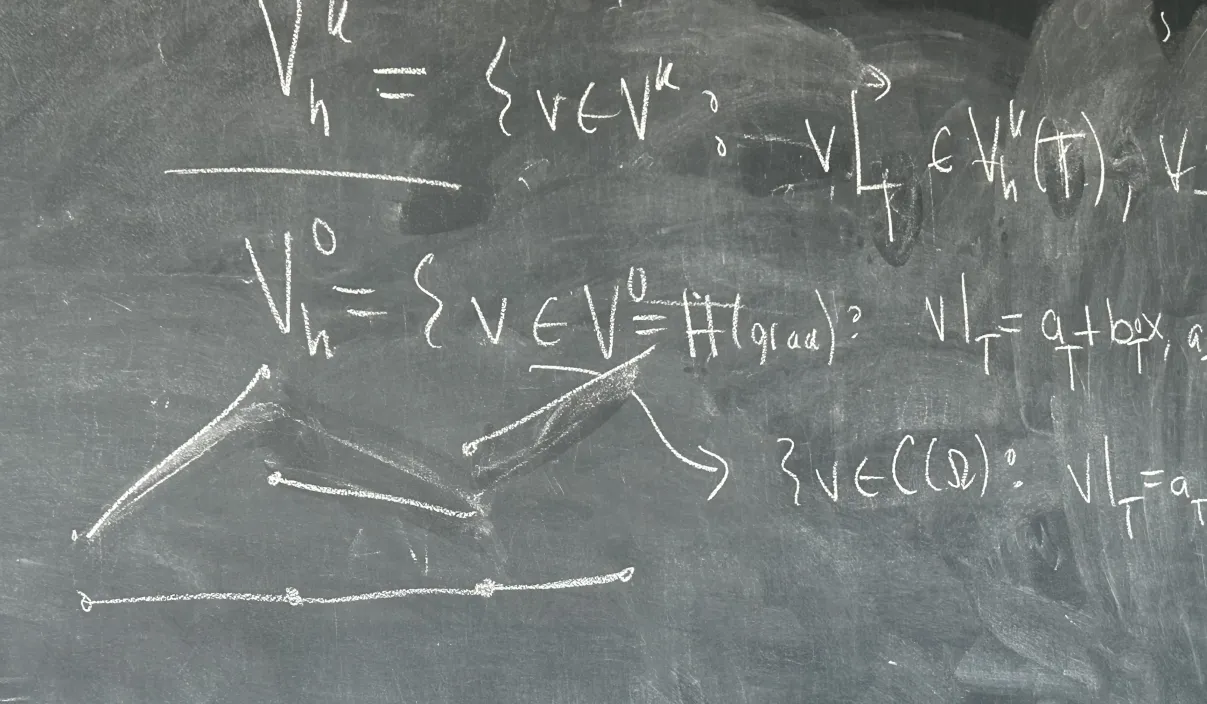
\includegraphics[width=0.5\textwidth]{Figures/lec3-1.png}\]
    The gradient is not actually a function, its weak derivative here is the dirac delta at the discontinuities (so the function is not in $H^1$!). Therefore, we better let the function to be \textbf{CONTINUOUS} and piece-wise linear for its weak gradient to exist in $L^2$.
\end{example}

As another example, we have that
\[V^2_h = \{v \in V^2 = H(div): v|_T = a_T + b_T \vec{x}, a_T \in \Rbb^3, b_T \in \Rbb, \forall T \in \tau_h\}.\]
In this case, do we need the functions to be continuous? Not necessarily, it can alternatively be characterized as
\[V^2_h = \{v|_T =  a_T + b_T \vec{x}, a_T \in \Rbb^3, b_T \in \Rbb, v \cdot \eta \text{ is ``continuous" across all faces of the triangulation.}\}\]
where $\eta$ is normal to the face from one of the tetrahedrons. More precisely, the characterization above is that - let $F = \partial T \cap \partial K$ for $T, K \in \tau_h$, then $v|_K \circ \eta = v|_T \circ \eta$ on $F$. (Note that the second definition is not forcing $v \in H(div)$.)

\begin{proposition}
    These two definitions for $V^2_h$ are equivalent.
\end{proposition}

\begin{proof}
    Let $v \in V^2_h$ in the first definition, then we wish to show that $v \circ \eta$ is continuous across faces. Let $F$ be a face of $\tau_h$ with $F = \partial K \cap \partial T$. Let $\varphi \in C_0^\infty(T \cup K)$ be a smooth function vanishing on the boundary of $T \cup K$  (note that it could be non-zero on $\partial K \cap \partial T$ because of this). Taking integration by parts gives
    \begin{align*}
        \langle div(v), \varphi \rangle_{T \cup K} &= - \langle v, grad(\varphi) \rangle_{T \cup K} \tag*{$\varphi$ vanishes on the boundary}\\
        &= - \langle v, \grad \varphi\rangle_T - \langle v, \grad \varphi \rangle_{K}\\
        &= \langle div(v), \varphi \rangle_T - \langle v \circ \eta, \varphi \rangle_{\partial T} + \langle div(v), \varphi \rangle_K - \langle v \circ \eta, \varphi \rangle_{\partial K} \tag*{Integration by parts}.
    \end{align*}
    On the other hand, we know that 
    \[ \langle div(v), \varphi \rangle_{T \cup K} =  \langle div(v), \varphi \rangle_{T} +  \langle div(v), \varphi \rangle_{K}\]
    Hence, we have that
    \[\langle v \circ \eta, \varphi \rangle_{\partial K} + \langle v \circ \eta, \varphi \rangle_{\partial T} = 0.\]
    $\varphi$ vanishes on all other boundary components except for $F = \partial K \cap \partial T$, hence we can write the equation above as
    \[\int_F (v|_K - v|_T) \circ \eta (\varphi) = 0.\]
    Since $\varphi$ is arbitrary, by a density argument we have that
    \[(v|_K - v|_T ) \circ \eta = 0.\]
    The converse follows similarly by reversing the steps.
\end{proof}

\begin{lemma}
   Similarly, we can write $$V_h^0 = \{v: v|_T \in V^0_h(T), v \text{ is continuous across faces $F$}\}.$$
    $$V_h^1 = \{v: v|_T \in V^0_h(T), v \times \eta \text{ is continuous across faces $F$}\}.$$
   $$V^2_h = \{v: v|_T \in V^2_h(T), v \circ \eta \text{ is continuous across faces $F$}\}.$$
    $$V^3_h = \{v: v|_T \in V^3_h(T)\}.$$
   Note that for $V_h^0$, if it's continuous across all faces, it is globally continuous.
\end{lemma}

Let $S$ be a finite dimensional space, consider a linear functional $F: S \to \Rbb$. If $\dim S = m$, then the \textbf{degree of freedom} of $S$ are the $m$ unique functionals $\{F_1, ..., F_m\}$ such that if $F_i(v) = 0$ for all $i$, then $v = 0$.
\begin{remark}
    These $F_i$'s are precisely a dual basis.
\end{remark}

Here's an alternative way to think about this
\begin{definition}[Degrees of Freedom]
    Let $K$ be a tetrahedra and consider $V^0_h(K)$, the the degree of freedoms of $V^0_h(K)$ are exactly
    \[v \mapsto v(y_i), y_i \text{ is a vertex of $K$},\]
    which ranges through the $4$ vertices of tetrahedra.\\

    Now consider $V^1_h(K) = \{a + b \times x, a \in \Rbb^3, b \in \Rbb^3\}$. We can define the functions as
    \[\int_e v \circ t_e,\]
    for all six edges $e$ of $K$ and $t_e$ is a tangent vector on the edge. This actually uniquely determines $v$, though it might be somewhat involves to show this.\\

    Now consider $V^2_h(K) = \{a + bx, a \in \Rbb^3, b \in \Rbb\}$, then we define the functions as
    \[\int_F v \cdot \eta_F,\]
    for all faces $F$ of $K$ and $\eta_F$ is a normal vector to the space.\\

    Now consider $V^3_h(K) = \{a: a \in \Rbb\}$, then
    \[\int_K a \]
    over the tetrahedra uniquely determines the value.
\end{definition}

Let's work through one of the examples of the degree of freedom.
\begin{lemma}
    Let $v \in V^2_h(K) = \{a + b x: a \in \Rbb^3, b \in \Rbb\}$, then $v$ is uniquely determined by the following degrees of freedom
    \[\int_F v \cdot \eta_F, \]
    for all faces $F$ of $K$.
\end{lemma}

\begin{proof}
    Let's write 
    \[\int_{F_1} v \cdot n_1 = \gamma_1, \int_{F_2} v \cdot n_2 = \gamma_2, \int_{F_3} v \cdot n_3 = \gamma_3, \int_{F_4} v \cdot n_4 = \gamma_4.\]
    We know that $v = a + b x$ (recall one of them is a vector), so we have a linear system
    \[A \begin{pmatrix}
        a\\
        b
    \end{pmatrix} = \begin{pmatrix}
        \gamma_1\\
        \gamma_2\\
        \gamma_3\\
        \gamma_4
    \end{pmatrix}.\]
   where $A$ is some matrix to be determined what about take in $a, b$ (representing $v$) and output the $\gamma_i$'s to be determined. It suffices for us to show that $A$ is injective.\\

   Suppose $\gamma_i = 0$ for all $i$, then we seek to show that $v \equiv 0$. Now we claim that $v \cdot n_j$ is actually constant on $F_j$. This is because let $F$ be a face, $x_0$ be a vertex on $F$ and $x \in F$ is in the interior. Then $(x - x_0)$ is tangent to the plane $F$ and hence $(x - x_0 \cdot n = 0$, hence $x_0 \cdot n = x \cdot n$. Thus, we have that
   \[(a + bx) \cdot n_j = a \cdot n_j + b x \cdot n_j = a \cdot n_j + b x_0 \cdot n_j,\]
   which is always going to be a constant. Hence, the integral being zero implies that $v \cdot n_j$ must be zero on each face $F_j$. We have that by integration by parts.
\[\int_T div(v) = \int_{\partial T} v \cdot n = \sum_{i} \int_{F_i} v \cdot n_i = 0. \]
We also have that $div(v) = div(a + bx) = b div(x) = 3b$. Hence
\[3|T| b = 0 \implies b = 0.\]
Thus, we have that $v = a$ is just a constant vector. We know that $a \cdot n_i = 0$, any three of the $n_i$'s are linearly independent, so this implies that $a = 0$.
\end{proof}

\begin{remark}
    The argument for the curl is omitted as it is much more complicated, but later we will redo this in general dimensions.
\end{remark}

\begin{lemma}
    We have yet another equivalent formulation
    \[V^2_h = \{v: v|_T \in V^2_h(T), \forall T \in \tau_h \text{ and } \int_F v \cdot \eta \text{ is single valued for all faces $F$} \}.\]
    By single valued we mean $\int_F v|_K \cdot n = \int_F v|_T \cdot n$, the integral is the same.
\end{lemma}

 \begin{proof}
     To show the original implies this definition, we have that $\int_F v|_K \cdot n = \int_F v|_T \cdot n$ on $F = \partial K \cap \partial T$, then this implies that $v \cdot n$ is single valued on $F$ because we know that $v \cdot n$ is constant. Converse is similar.
 \end{proof}

We have yet another alternative characterization
\begin{lemma}
    $V^1_h = \{v \in V|_T \in V^1_h(T), \forall T \in \tau_h \text{ and } \tau_e v \cdot t_e \text{ is single-valued}\}$. In other words, for any tetrahedron neighboring $e$, its restriction of $v$ to each edge gives the same integral.
\end{lemma}

\begin{proof}
    Exercise.
\end{proof}

Recall that $S^0 = S^3 = C^\infty(\overline{\Omega}), S^1 = S^2 = [C^\infty(\overline{\Omega})]^3$, then we define
\begin{definition}
    Let $I^k_h: S^k \to V^k_h$ be defined as the unique function corresponding to the functional:
    \[(I_h^0 v)(y) = v(y),\]
    for all vertices $y$ (ie. we specify its value at the four vertices and find the corresponding affine function).\\

    Similarly, we also define $I^1_h v$ as the unique function in $V^1_h$ satisfying
    \[\int_e (I^1_n v) \cdot t_e = \int_e v \cdot t_e,\]
    for all edges.

    We define $I^2_h v$ as the unique function in $V^2_h$ satisfying
    \[\int_F I^2_h v \cdot n = \int_F v \cdot n. \]

    We define $I^3_h v$ as the unique function in $V^3_h$ satisfying
    \[\int_K I^3_h v = \int_{K} v.\]
\end{definition}

Now we have defined the maps
% https://q.uiver.app/#q=WzAsOCxbMCwwLCJTXjAiXSxbMSwwLCJTXjEiXSxbMiwwLCJTXjIiXSxbMywwLCJTXjMiXSxbMCwxLCJWXjBfaCJdLFsxLDEsIlZeMV9oIl0sWzIsMSwiVl4yX2giXSxbMywxLCJWXjNfaCJdLFswLDQsIkleMF9oIl0sWzEsNSwiSV4xX2giXSxbMiw2LCJJXjJfaCJdLFszLDcsIkleM19oIl0sWzAsMSwiZF4wIl0sWzEsMiwiZF4xIl0sWzIsMywiZF4yIl0sWzQsNSwiZF4wIiwyXSxbNSw2LCJkXjEiLDJdLFs2LDcsImReMiIsMl1d
\[\begin{tikzcd}
	{S^0} & {S^1} & {S^2} & {S^3} \\
	{V^0_h} & {V^1_h} & {V^2_h} & {V^3_h}
	\arrow["{I^0_h}", from=1-1, to=2-1]
	\arrow["{I^1_h}", from=1-2, to=2-2]
	\arrow["{I^2_h}", from=1-3, to=2-3]
	\arrow["{I^3_h}", from=1-4, to=2-4]
	\arrow["{d^0}", from=1-1, to=1-2]
	\arrow["{d^1}", from=1-2, to=1-3]
	\arrow["{d^2}", from=1-3, to=1-4]
	\arrow["{d^0}"', from=2-1, to=2-2]
	\arrow["{d^1}"', from=2-2, to=2-3]
	\arrow["{d^2}"', from=2-3, to=2-4]
\end{tikzcd}\]

\textbf{Claim: } This diagram in fact commutes. We will post pone this to next lecture.

\begin{definition}
    We define the $k$-th de Rham cohomology as
    \[H^k_S = \operatorname{ker}(d^k, S^k)/\operatorname{Range}(d^{k-1}, S^{k-1}),\]
    where we say $v \sim q$ if $v - q = d^{k-1} e$ for some $e \in S^{k-1}$. We could similarly define the quotients for $V^k$ (denoted $H^k_V$) and $V^k_h$ (denoted $H^k_h$). 
\end{definition}

It turns out that these three cohomologies are all isomorphic! We first claim that $I^k_h$ gives a well-defined map between $H^k$ to $H^k_h$. Indeed, suppose $v \in H^k$ such that $d^k(v) = 0$, then by the commutativity of the diagram shows $d^k(I^k_n(v)) = I^{k+1}_n (d^k v) = 0$. Hence $I^k_n(v)$ is actually in the kernel. This map is also well-defined up to coboundary (will be shown next time). This gives a well-defined map $I^k_h: H^k_S \to H^k_h$.

\subsection{De Rham's Theorem}

This leads to the following theorem which we will prove later:

\begin{theorem}[De Rham's Theorem]
    $I^k_h: H^k_S \to H^k_h$ is an isomorphism.
\end{theorem}

Now given a triangulation $\tau_h$ let $\Delta_k$ be the collection of all $k$ sub0simplicies in $\tau_h$. Consider 
\[\sigma = [x_0, x_1, ..., x_k],\]
where $x_i$ are the vertices of $\sigma$. We \textbf{identify an orientation on $\sigma$} in the sense that
\[-\sigma = [x_1, ..., x_j, ...., x_i, ..., x_k],\]
where we swapped $i$ and $j$. Swapping twice gives the positive sign again etc.

\begin{definition}
    The $k$-chains are the formal $\Rbb$-linear combinations of $k$-subsimplicies
    \[C_k = \{\sum_{\sigma \in \Delta_k} a_\sigma \sigma, a_\sigma \in \Rbb\}.\]
    We define a boundary map $\partial_k: C_k \to C_{k-1}$ that is linear. We define how it acts on the basis as
    \[\partial_k([x_0, ..., x_k]) = \sum_{j = 0}^k (-1)^j [x_0, ..., \hat{x_j}, ..., x_k].\]
\end{definition}

\begin{lemma}
    $\partial_{k-1} \circ \partial_k$ is the zero map.
\end{lemma}

\begin{proof}
    We can check this on the basis elements. Indeed,
    \begin{align*}
        \partial_{k-1} \circ \partial_k([x_0, ..., x_k]) &= \partial_{k-1} \left(\sum_{j = 0}^k (-1)^j [x_0, ..., \hat{x}_j, ..., x_k]\right)\\
        &= \sum_{\ell \leq j-1} \sum_j (-1)^{j+\ell} [x_0, ..., \hat{x}_\ell, ..., \hat{x}_j, ..., x_k] + \sum_{\ell \geq j+1} \sum_j (-1)^{j+\ell - 1} [x_0, ..., \hat{x}_j, ..., \hat{x}_\ell, ..., x_k]\\
        &=\sum_{\ell \leq j-1} \sum_j (-1)^{j+\ell} [x_0, ..., \hat{x}_\ell, ..., \hat{x}_j, ..., x_k] + \sum_{j \leq \ell-1} \sum_\ell (-1)^{j+\ell - 1} [x_0, ..., \hat{x}_j, ..., \hat{x}_\ell, ..., x_k]
    \end{align*}
    Convince yourself that these two sums are the same but differ by a sign, so they cancel each other and gives us $0$.
\end{proof}

This gives us the maps
% https://q.uiver.app/#q=WzAsNyxbMSwwLCJDXzAiXSxbMiwwLCJDXzEiXSxbMywwLCJDXzIiXSxbNCwwLCJDXzMiXSxbNSwwLCIwIl0sWzYsMCwiLi4uIl0sWzAsMCwiMCJdLFs0LDNdLFs1LDRdLFswLDYsIlxccGFydGlhbF8wIl0sWzEsMCwiXFxwYXJ0aWFsXzEiXSxbMiwxLCJcXHBhcnRpYWxfMiJdLFszLDIsIlxccGFydGlhbF8zIl1d
\[\begin{tikzcd}
	0 & {C_0} & {C_1} & {C_2} & {C_3} & 0 & {...}
	\arrow[from=1-6, to=1-5]
	\arrow[from=1-7, to=1-6]
	\arrow["{\partial_0}", from=1-2, to=1-1]
	\arrow["{\partial_1}", from=1-3, to=1-2]
	\arrow["{\partial_2}", from=1-4, to=1-3]
	\arrow["{\partial_3}", from=1-5, to=1-4]
\end{tikzcd}\]
which gives us the homology. Dualizing the complexes, we define
\[C^k = \Hom(C_k, \Rbb).\]

Now, given $\sigma \in \Delta_k$, we can define the dual basis $\sigma^* \in C^k$ as
\[\sigma^*(\tau) = \begin{cases}
    0, \text{ if $\tau$ is not a permutation of $\sigma$}\\
    \pm 1, \text{ if $\tau = \pm \sigma$}
\end{cases}\]
This gives a dual basis in $C^k$ (where we call the spaces $C^k$ \textbf{cochains}). Then we define the \textbf{coboundary operator} $d^k: C^k \to C^{k+1}$ as
\[d^k X(\sigma) = X(\partial_{k+1} \sigma),\]
for all $X \in C^k$ and $\sigma \in C_{k+1}$.\\

Concretely, for $\sigma \in \Delta_k$, we have that
\[d^k \sigma^* = \sum_{x \in \Delta_0, [x, \sigma] \in \Delta_{k+1}} [x \sigma]^*.\]

\newpage
\section{Lecture Feburary 21st}

The regular lecture on February 14th was cancelled, but there was a talk on applications of exterior calculus.

\subsection{Commutativity of the Diagram}

Last time, we define $I^k_h: S^k \to V^k_h$ such that, for each $k$, it is the unique functional satisfying
\begin{itemize}
    \item $(I^0_h v)(y) = v(y)$ where each $y \in \mathcal{V}_h$ (\text{ vertices}).
    \item $\int_e (I^1_h v) \cdot t = \int_e v \cdot t$, for $e \in \mathcal{E}_n$ (edges).
    \item $\int_F (I^2_h v) \cdot \eta = \int_F v \cdot \eta$, for $F \in \mathcal{F}_h$ (faces).
    \item $\int_T I^3_h v = \int_T v$, for $T \in \tau_h$ (tetrahedrons).
\end{itemize}

In particular, we defined the map of chain complexes
% https://q.uiver.app/#q=WzAsOCxbMCwwLCJTXjAiXSxbMSwwLCJTXjEiXSxbMiwwLCJTXjIiXSxbMywwLCJTXjMiXSxbMCwxLCJWXjBfaCJdLFsxLDEsIlZeMV9oIl0sWzIsMSwiVl4yX2giXSxbMywxLCJWXjNfaCJdLFswLDQsIkleMF9oIl0sWzEsNSwiSV4xX2giXSxbMiw2LCJJXjJfaCJdLFszLDcsIkleM19oIl0sWzAsMSwiZF4wIl0sWzEsMiwiZF4xIl0sWzIsMywiZF4yIl0sWzQsNSwiZF4wIiwyXSxbNSw2LCJkXjEiLDJdLFs2LDcsImReMiIsMl1d
\[\begin{tikzcd}
	{S^0} & {S^1} & {S^2} & {S^3} \\
	{V^0_h} & {V^1_h} & {V^2_h} & {V^3_h}
	\arrow["{I^0_h}", from=1-1, to=2-1]
	\arrow["{I^1_h}", from=1-2, to=2-2]
	\arrow["{I^2_h}", from=1-3, to=2-3]
	\arrow["{I^3_h}", from=1-4, to=2-4]
	\arrow["{d^0}", from=1-1, to=1-2]
	\arrow["{d^1}", from=1-2, to=1-3]
	\arrow["{d^2}", from=1-3, to=1-4]
	\arrow["{d^0}"', from=2-1, to=2-2]
	\arrow["{d^1}"', from=2-2, to=2-3]
	\arrow["{d^2}"', from=2-3, to=2-4]
\end{tikzcd}\]

\begin{proposition}
We will now check that the small squares commute
\[I^1_h \circ \grad = \grad \circ I^0_h,\]
\[I^2_h \circ \curl = \curl \circ I^1_h,\]
\[I^3_h \circ \operatorname{div} = \operatorname{div} \circ I^2_h.\]    
\end{proposition}

\begin{proof}
    All of these follows from integration by parts. We will generalize this to an arbitrary dimension later, so we will just prove the first equality for demonstration. Indeed, for any $v \in S^0$, we seek to show that 
    \[I^1_h \circ \grad = \grad \circ I^0_h.\]
    A function in $V^1_h$ is uniquely determined by its edges. Hence, it suffices for us to integrate them against edges and show that they are equal, ie.
    \[\int_e (I^1_h \circ \grad)(v) \cdot t = \int_e (\grad \circ I^0_h v) \cdot t, \forall e \in \mathcal{E}_h.\]
    Lets call the LHS as $M_1$ and the RHS as $M_2$. Now we have that
    \begin{align*}
        M_1 &= \int_e (I^1_h \circ \grad)(v) \cdot t \\
        &= \int_e \grad(v) \cdot t \tag*{Definition of $I^1_h$}.
    \end{align*}
    Write the edge $e = [x_0, x_1]$ and we can take $t = \frac{x_1 - x_0}{|x_1 - x_0|}$ unit tangent to the edge, then we have that
    \begin{align*}
        M_1 &= \int_e \grad(v) \cdot t\\
        &= \int_{e} \partial_t v\\
        &= v(x_1) - v(x_0) \tag*{Fundamental Theorem of Calculus}
    \end{align*}
    Similarly, for $M_2$, we have that
    \begin{align*}
        M_2 &= \int_e (\grad I^0_h v) \cdot t\\
        &= \int_e \partial_t (I^0_h v)\\
        &= I^0_h(v(x_1)) - I^0_h(v(x_0))\\
        &= v(x_1) - v(x_0) \tag*{By definition of $I^0_h$}
    \end{align*}
    The proofs for the other two squares follow similarly, they are a bit more involved but not too much.
\end{proof}

\subsection{Chains and Cochain Complex}

Recall that we have also defined last time the chain complexes
\[C_k = \{ \sum_{\sigma \in \overline{\Delta_k}} a_\sigma \sigma: a_\sigma \in \Rbb \}, \]
where $\Delta_k$ is the set of oriented $k$-simplicies in our mesh $\tau_h$ and (to be precise) 
\[\overline{\Delta_k} = \{[y_{i_0}, ..., y_{i_k}], i_0 < i_1 < ... < i_k\},\]
where we fix the indices to be increasing (this avoids worrying about its permutation).\\

We also defined the boundary map
\[\partial_k: C_k \to C_{k-1},\]
where given $\sigma = [x_0, ..., x_k]$, we have that
\[\partial_k \sigma = \sum_{j = 0}^k (-1)^j [x_0, ..., \hat{x_j}, ..., x_k].\]

\begin{example}
    If we take $\sigma = [x_0, x_1, x_2]$, then
    \[\partial_2 \sigma = [x_1, x_2] - [x_0, x_2] + [x_0, x_1].\]
    An interpretation of this orientation is that $[x_1, x_2]$ goes from $x_1$ to $x_2$. $-[x_0, x_2]$ goes from $x_2$ to $x_0$, and $[x_0, x_1]$ goes from $x_0$ to $x_1$. This gives an orientation on $\sigma$.
\end{example}

Last time, we proved that $(C_k, \partial_k)$ does indeed form a chain complex.
\begin{lemma}
    $\partial_{k-1} \circ \partial_k = 0$.
\end{lemma}

Hence, we can build a chain complex
% https://q.uiver.app/#q=WzAsNyxbMSwwLCJDXzAiXSxbMiwwLCJDXzEiXSxbMywwLCJDXzIiXSxbNCwwLCJDXzMiXSxbNSwwLCIwIl0sWzYsMCwiLi4uIl0sWzAsMCwiMCJdLFs0LDNdLFs1LDRdLFswLDYsIlxccGFydGlhbF8wIl0sWzEsMCwiXFxwYXJ0aWFsXzEiXSxbMiwxLCJcXHBhcnRpYWxfMiJdLFszLDIsIlxccGFydGlhbF8zIl1d
\[\begin{tikzcd}
	0 & {C_0} & {C_1} & {C_2} & {C_3} & 0 & {...}
	\arrow[from=1-6, to=1-5]
	\arrow[from=1-7, to=1-6]
	\arrow["{\partial_0}", from=1-2, to=1-1]
	\arrow["{\partial_1}", from=1-3, to=1-2]
	\arrow["{\partial_2}", from=1-4, to=1-3]
	\arrow["{\partial_3}", from=1-5, to=1-4]
\end{tikzcd}\]
We can dualize these complexes by defining $C^k = \Hom(C_k, \Rbb)$ as the \textbf{cochain complexes}. Concretely, for each $k$-chain $\sigma$, we can define $\sigma^* \in C^k$ as
\[\sigma^*(\tau) = \begin{cases}
    0, \text{ if $\tau \in \overline{\Delta_k}$ is not a permutation of $\sigma$}\\
    1, \text{ if $\tau \in \overline{\Delta_k}$ and $\tau = \sigma$}
\end{cases}\]
Note that $\tau$ is a permutation of $\sigma$ (which willnot be $\overline{\Delta_k}$) we give $-1$ for odd permutation and $+1$ for even. We can extend $\sigma^*$ $\Rbb$-linearly as $\sigma^*(\sum_{\tau \in \Delta_k} a_\tau \tau) = \sum_{\tau \in \Delta_k} a_\tau \sigma^*(\tau)$.\\

For any $X \in C^k$, we can write
\[X = \sum_{\sigma \in \overline{\Delta_k}} X(\sigma) \sigma^*.\]
\begin{definition}
From here we define the \textbf{coboundary operator}
\[d^k: C^k \to C^{k+1}, d^k X(\sigma) = X(\partial_{k+1} \sigma), \text{ where $\sigma \in C_{k+1}$ \text{ and } $X \in C^k$}. \]
\end{definition}

\begin{proposition}
There's a very nice formula that expresses the coboundary operator concretely, we only need to check this on the basis. Given $\sigma = [x_0, x_1, ..., x_k] \in \Delta_k$, one can check that
\[d^k \sigma^* = \sum_{x \in \Delta_0, [x, x_0, ..., x_k] \in \Delta_{k+1}} [x, x_0, ..., x_k]^*\]    
\end{proposition}

\begin{proof}
    We only check this for $k = 0$, but the other cases follow by honest computation. Indeed, let $\sigma = [x_0]$, then we have that
    \[d^0 \sigma^* = [v_1, x_0]^* + ... + [v_n, x_0]^*,\]
    where $v_1, ..., v_n$ are all the vertices with an edge to $x_0$. Now we check that
    \[[v_1, x_0]^* + ... + [v_n, x_0]^* = d^0 \sigma^*(\tau) = \sigma^*(\partial_1 \tau), \forall \tau \in C_{1}.\]
    Clearly if $\tau$ is not an edge with vertex $[x_0]$, it would evaluate to zero and we are good. If $\tau$ is an edge $[v_i, x_0]$ or $[x_0, v_i]$, then clearly $[v_1, x_0]^* + ... + [v_n, x_0]^*$ and $\sigma^*(\partial_1 \tau)$ both gives the same output.
\end{proof}

Now we will show that this is indeed a cochain complex.
\begin{lemma}
    $d^{k+1} \circ d^k = 0$.
\end{lemma}

\begin{proof}
    We have that for all $X \in C^k$ and $\tau \in C_{k+2}$, we have that
    \begin{align*}
        (d^{k+1} \circ d^k X)(\tau) &= (d^k X)(\partial_{k+2} \tau)\\
        &= X(\partial_{k+1} \circ \partial_{k+2} \tau)\\
        &= X(0)\\
        &= 0.
    \end{align*}
\end{proof}

Hence, we have also obtained a cochain complex
% https://q.uiver.app/#q=WzAsNixbMCwwLCIwIl0sWzEsMCwiQ14wIl0sWzIsMCwiQ14xIl0sWzMsMCwiQ14yIl0sWzQsMCwiQ14zIl0sWzUsMCwiMCJdLFswLDFdLFsxLDIsImReMCJdLFsyLDMsImReMSJdLFszLDQsImReMiJdLFs0LDUsImReMyJdXQ==
\[\begin{tikzcd}
	0 & {C^0} & {C^1} & {C^2} & {C^3} & 0
	\arrow[from=1-1, to=1-2]
	\arrow["{d^0}", from=1-2, to=1-3]
	\arrow["{d^1}", from=1-3, to=1-4]
	\arrow["{d^2}", from=1-4, to=1-5]
	\arrow["{d^3}", from=1-5, to=1-6]
\end{tikzcd}\]

\subsection{The De Rham Maps}

We have a map $R^k: S^k \to C^k$. For each $k$, we define the \textbf{De Rham map} $R^k v$ as the unique function in $C^k$ given by
\begin{itemize}
    \item $(R^0 v)(y) = v(y)$ for all $y \in \Delta_0$. (Note that $v \in C^\infty(\Omega)$)
    \item $(R^1 v)(e) = \int_\sigma v \cdot t$ for all $e \in \Delta_1$. (Note that $v \in [C^\infty(\Omega)]^3$)
    \item $(R^2 v)(F) = \int_F v \cdot \eta$ for all $F \in \Delta_2$. (Note that $v \in [C^\infty(\Omega)]^3$)
    \item $(R^3 v)(T) = \int_T v$ for all $T \in \Delta_3$. (Note that $v \in C^\infty(\Omega)$)
\end{itemize}
We again obtain a map of chain complexes
% https://q.uiver.app/#q=WzAsMTIsWzAsMSwiMCJdLFsxLDEsIkNeMCJdLFsyLDEsIkNeMSJdLFszLDEsIkNeMiJdLFs0LDEsIkNeMyJdLFs1LDEsIjAiXSxbMCwwLCIwIl0sWzEsMCwiU14wIl0sWzIsMCwiU14xIl0sWzMsMCwiU14yIl0sWzQsMCwiU14zIl0sWzUsMCwiMCJdLFswLDFdLFsxLDIsImReMCJdLFsyLDMsImReMSJdLFszLDQsImReMiJdLFs0LDUsImReMyJdLFs2LDddLFs3LDgsImReMCJdLFs4LDksImReMSJdLFs5LDEwLCJkXjIiXSxbMTAsMTEsImReMyJdLFs3LDEsIlJeMCJdLFs4LDIsIlJeMSJdLFs5LDMsIlJeMiJdLFsxMCw0LCJSXjMiXV0=
\[\begin{tikzcd}
	0 & {S^0} & {S^1} & {S^2} & {S^3} & 0 \\
	0 & {C^0} & {C^1} & {C^2} & {C^3} & 0
	\arrow[from=2-1, to=2-2]
	\arrow["{d^0}", from=2-2, to=2-3]
	\arrow["{d^1}", from=2-3, to=2-4]
	\arrow["{d^2}", from=2-4, to=2-5]
	\arrow["{d^3}", from=2-5, to=2-6]
	\arrow[from=1-1, to=1-2]
	\arrow["{d^0}", from=1-2, to=1-3]
	\arrow["{d^1}", from=1-3, to=1-4]
	\arrow["{d^2}", from=1-4, to=1-5]
	\arrow["{d^3}", from=1-5, to=1-6]
	\arrow["{R^0}", from=1-2, to=2-2]
	\arrow["{R^1}", from=1-3, to=2-3]
	\arrow["{R^2}", from=1-4, to=2-4]
	\arrow["{R^3}", from=1-5, to=2-5]
\end{tikzcd}\]

\begin{lemma}
    The diagram commutes, ie.
    \[d^k \circ R^k = R^{k+1} \circ d^k.\]
\end{lemma}

\begin{proof}
    We only show that for $k = 0$, but the proofs follow similarly for the maps $I^h_k$. Now we seek for show that, for all $v \in S^0$,
    \[d^0 R^0(v) = R^1 d^0(v).\]
    Now we know that $d^0(v) = \grad(v)$ (if we unwrap the definition). Hence we want to check that
    \[(d^0 R^0 v)(e) = R^1(\grad(v))(e), \quad \forall e \in \Delta_1.\]
    In this case, we have that
    \begin{align*}
        RHS &= \int_e (\grad v) \cdot t\\
        &= v(x_1) - v(x_0), \tag*{$e = [x_0, x_1]$}
    \end{align*}
    We also have that
    \begin{align*}
        LHS &= (d^0 R^0 v)(e)\\
        &= (R^0 v)(\partial_1 e)\\
        &= (R^0 v)([x_1] - [x_0])\\
        &= (R^0 v)([x_1]) - (R^0 v)([x_0])\\
        &= v(x_1) - v(x_0).
    \end{align*}
\end{proof}

Hereafter (at least in this lecture), we will define the
\begin{itemize}
    \item \textbf{Simplicial cohomology} groups as $H^k_h(\Delta) = \ker(d^k, C^k) /\operatorname{Range}(d^{k-1}, C^{k-1})$. We write kernel as $\mathcal{Z}^k_h(\Delta)$ and image as $B^k_h(\Delta)$.
    \item \textbf{De Rham Cohomology} groups as $H^k_S = \ker(d^k, S^k) / \operatorname{Range}(d^{k-1}, S^{k-1})$.
\end{itemize}

\begin{theorem}[De-Rham's Theorem]
    $R^k$ induces an isomorphism $H^k_S$ to $H^k_h(\Delta)$. 
\end{theorem}

We will prove this in general dimensions later, so we will ignore the map later. We also have the maps $I^k_h$'s called the \textbf{Nédélec interpolators} that people in analysis of PDEs care about more.
\[\begin{tikzcd}
	{S^0} & {S^1} & {S^2} & {S^3} \\
	{V^0_h} & {V^1_h} & {V^2_h} & {V^3_h}
	\arrow["{I^0_h}", from=1-1, to=2-1]
	\arrow["{I^1_h}", from=1-2, to=2-2]
	\arrow["{I^2_h}", from=1-3, to=2-3]
	\arrow["{I^3_h}", from=1-4, to=2-4]
	\arrow["{d^0}", from=1-1, to=1-2]
	\arrow["{d^1}", from=1-2, to=1-3]
	\arrow["{d^2}", from=1-3, to=1-4]
	\arrow["{d^0}"', from=2-1, to=2-2]
	\arrow["{d^1}"', from=2-2, to=2-3]
	\arrow["{d^2}"', from=2-3, to=2-4]
\end{tikzcd}\]

\subsection{The Whitney Map}

\begin{definition}[The Whitney Map on Simplex]
    For $\tau \in \overline{\Delta}_k$, we define $\phi_\tau \in V^k_h$ with the following property
    \[R^k \varphi_\tau = \tau^*.\]
\end{definition}

\begin{example}[For $k = 0$]
    When $k = 0$, we have that $\tau = [x_0]$ and for all $y \in \overline{\Delta}_0$.
    \[(R^0 \varphi_\tau))(y) = \varphi_\tau(y),\]
    by definition of $R^0$. On the other hand, the Whitney map specifies that
    \[(R^0 \varphi_\tau))(y) = \tau^*(y) = [x_0]^*(y) = \begin{cases}
        1, y = x_0\\
        0, y \neq x_0
    \end{cases}.\]
    Hence we want a map $\varphi_\tau$ to be the unique map in $V^0_h$ determined by
    \[\varphi_{\tau}(y) = \begin{cases}
        1, y = x_0\\
        0, y \neq x_0
    \end{cases}.\]
    In finite element methods, these are called \textbf{the hat functions} (the unique piecewise affine function that is globally continuous, $1$ on $y$, and zero on all other vertices).
\end{example}

\begin{example}[For $k = 1$]
    When $k = 1$, we have that $\tau = [x_0, x_1]$, and for eveyr edge $e$, we have that
    \[(R^1 \varphi_\tau)(e) = \tau^*(e) = \begin{cases}
        1, \tau = e, e \in \overline{\Delta}_1\\
        0, \tau \neq e, e \in \overline{\Delta}_1
    \end{cases},\]
    On the other hand, we also have that
    \[R^1(\varphi_\tau)(e) = \int_e \varphi_\tau \cdot t.\]
    Hence, $\varphi_\tau$ is the unique function in $V^1_h$ satisfying
    \[\int_e \varphi_\tau \cdot t = \begin{cases}
        1, \tau = e, e \in \overline{\Delta}_1\\
        0, \tau \neq e, e \in \overline{\Delta}_1
    \end{cases}.\]
    Note that $\varphi_\tau$ has support on all the triangles bounding the edge $\tau$ and vanish outside of these triangles. Note that $\varphi_\tau$ is not necessarily continuous as it's in $V^1_h$ (only its tangential components have to be continuous).
\end{example}

\begin{example}[For $k = 2, 3$]
    When $k = 2$, $\tau = [x_0, x_1, x_2]$, we have similarly that
    \[\int_F \varphi_\tau \cdot \eta = \begin{cases}
        1, F = \tau\\
        0, F \neq \tau
    \end{cases}.\]
    When $K = 3$, $\tau = [x_0, x_1, x_2, x_3]$, we have similarly that
    \[\int_T \varphi_\tau = \begin{cases}
        1, F = \tau\\
        0, F \neq \tau
    \end{cases}.\]
\end{example}

\begin{definition}[The Whitney Map]
    We define the Whitney map $W_k: C^k \to V^k_h$ given by
    \[W_k(X) = \sum_{\sigma \in \overline{\Delta}_k} X(\sigma) \varphi_\sigma.\]
    By construction, clearly this is injective. Since both spaces have the same dimensional and are finite dimensional, this is surjective. Hence, this is an isomorphism.
\end{definition}

We extend the definition of $R^k$ to be on $V^k_h$ by considering:
\[(R^0 v)(y) = v(y),\]
and so on. Note that we can do this because we did not actually use the property that the function is smooth (we only needed them to have well-defined values for integrals on vertex, edges, faces, and tetrahedrons, etc.)

\begin{lemma}
$R_k \circ W_k = \operatorname{Identity}$, where $R_k$ in this case is from $V^k_h$.
\end{lemma}

\begin{proof}
    We have that $R^k \circ W_k(X) = X$ if and only if $R^k W_k(\sigma^*) = \sigma^*$ for all $\sigma$. Indeed, we have exactly
    \[R^k \circ \varphi_\sigma = \sigma^*\]
    This follows directly from how we constructed them.
\end{proof}

\begin{lemma}
    $I^k_h = W_k \circ R^k$, where $R^k$ in this case is from $S^k$.
\end{lemma}

\begin{proof}
    We seek to show that $I^k_h v = W_k R^k v$ for all $v \in S^k$. For the case that $k = 1$, we seek to show that
    \[\int_e (I^1_h v) \cdot t = \int_e (W_1 R^1 v) \cdot t,\]
    for all $e \in \overline{\Delta}_1$. The LHS by definition is just $\int_e v \cdot t$. Now we know that 
    \[(R^1 v) = \sum_{\sigma \in \overline{\Delta}_1} (R^1 v)(\sigma) \sigma^*\]
    Hence we have that
    \[W_1 R^1 v = \sum_{\sigma \in \overline{\Delta}_1} (R^1 v)(\sigma) \varphi_\sigma = \sum_{\sigma \in \overline{\Delta}_1} (R^1 v)(\sigma) \delta_{e, \sigma},\]
    which is the exact same as $\int_e v \cdot t$. The other cases are omitted.
\end{proof}

\begin{proposition}
    The following diagram
% https://q.uiver.app/#q=WzAsMTgsWzAsMiwiMCJdLFsxLDIsIlZeMF9oIl0sWzIsMiwiVl4xX2giXSxbMywyLCJWXjJfaCJdLFs0LDIsIlZeM19oIl0sWzUsMiwiMCJdLFswLDEsIjAiXSxbMSwxLCJDXjAiXSxbMiwxLCJDXjEiXSxbMywxLCJDXjIiXSxbNCwxLCJDXjMiXSxbNSwxLCIwIl0sWzEsMCwiU14wIl0sWzIsMCwiU14xIl0sWzMsMCwiU14yIl0sWzQsMCwiU14zIl0sWzUsMCwiMCJdLFswLDAsIjAiXSxbMCwxXSxbMSwyLCJkXjAiXSxbMiwzLCJkXjEiXSxbMyw0LCJkXjIiXSxbNCw1LCJkXjMiXSxbNiw3XSxbNyw4LCJkXjAiXSxbOCw5LCJkXjEiXSxbOSwxMCwiZF4yIl0sWzEwLDExLCJkXjMiXSxbNywxLCJXXjAiXSxbOCwyLCJXXjEiXSxbOSwzLCJXXjIiXSxbMTAsNCwiV14zIl0sWzE3LDEyXSxbMTIsMTMsImReMCJdLFsxMywxNCwiZF4xIl0sWzE0LDE1LCJkXjIiXSxbMTUsMTYsImReMyJdLFsxNSwxMCwiUl4zIl0sWzE0LDksIlJeMiJdLFsxMiw3LCJSXjAiXSxbMTMsOCwiUl4xIl1d
\[\begin{tikzcd}
	0 & {S^0} & {S^1} & {S^2} & {S^3} & 0 \\
	0 & {C^0} & {C^1} & {C^2} & {C^3} & 0 \\
	0 & {V^0_h} & {V^1_h} & {V^2_h} & {V^3_h} & 0
	\arrow[from=3-1, to=3-2]
	\arrow["{d^0}", from=3-2, to=3-3]
	\arrow["{d^1}", from=3-3, to=3-4]
	\arrow["{d^2}", from=3-4, to=3-5]
	\arrow["{d^3}", from=3-5, to=3-6]
	\arrow[from=2-1, to=2-2]
	\arrow["{d^0}", from=2-2, to=2-3]
	\arrow["{d^1}", from=2-3, to=2-4]
	\arrow["{d^2}", from=2-4, to=2-5]
	\arrow["{d^3}", from=2-5, to=2-6]
	\arrow["{W_0}", from=2-2, to=3-2]
	\arrow["{W_1}", from=2-3, to=3-3]
	\arrow["{W_2}", from=2-4, to=3-4]
	\arrow["{W_3}", from=2-5, to=3-5]
	\arrow[from=1-1, to=1-2]
	\arrow["{d^0}", from=1-2, to=1-3]
	\arrow["{d^1}", from=1-3, to=1-4]
	\arrow["{d^2}", from=1-4, to=1-5]
	\arrow["{d^3}", from=1-5, to=1-6]
	\arrow["{R^3}", from=1-5, to=2-5]
	\arrow["{R^2}", from=1-4, to=2-4]
	\arrow["{R^0}", from=1-2, to=2-2]
	\arrow["{R^1}", from=1-3, to=2-3]
\end{tikzcd}\]
commutes.
\end{proposition}

\begin{proof}
    We know $I^k_h$ and $R^k$ are chain maps, so it suffices to show that $W_k$ is a chain map. Now we want to show that
    \[d^k W_k = W_{k+1} d^k,\]
    so we have that this is true if and only if
    \[R^{k+1} d^k W_k = R^{k+1} W_{k+1} d^k,\]
    which is true if and only if (by commutativity of diagram)
    \[d^k (R^k W_k) = (R^{k+1} W_{k+1}) d^k, \]
    where we know from lemma $R^k W_k$ and $R^{k+1} W_{k+1}$ are both identities.
\end{proof}


\newpage
\section{Lecture February 28th}

\subsection{Exterior Calculus}

Let $(\Rbb^n)^*$ be the space of linear functionals on $\Rbb^n$.

\begin{definition}
    Let $\phi_1, ..., \phi_n \in \Rbb^n$, we define the \textbf{wedge product} of the linear functions as a $k$-linear map (meaning that it is linear in each coordinate)
    \[\phi_1 \wedge ... \wedge \phi_n: \Rbb^n \times ... \times \Rbb^n \to \Rbb,\]
    such that for any $(v_1, ..., v_k) \in \Rbb^n \times ... \times \Rbb^n$, we have that
    \[(\phi_1 \wedge ... \wedge \phi_n)(v_1, ..., v_k) = \det A,\]
    where $A$ is a $k \times k$ matrix 
    \[A = \begin{pmatrix}
        \phi_1(v_1) & ... & \phi_1(v_k)\\
        \vdots & \ddots & \vdots\\
        \phi_k(v_1) & ... & \phi_k(v_k)
    \end{pmatrix}.\]
\end{definition}

One can check that the wedge product is linear in each coordinate and that for any permutation $\sigma \in S_k$, we have that
    \[(\phi_1 \wedge ... \wedge \phi_n)(v_{\sigma(1)}, ..., v_{\sigma(k)}) = \operatorname{sign}(\sigma)(\phi_1 \wedge ... \wedge \phi_n)(v_1, ..., v_k). \]
Furthermore, if any $v_i = v_j$ for $i \neq j$, we have that 
\[(\phi_1 \wedge ... \wedge \phi_n)(v_1, ..., v_k) = \det A = 0.\]

Let $e_1, ..., e_n$ be the canonical basis of $\Rbb^n$ (ie. $e_1 = (1, 0, ..., 0)$, ..., $e_n = (0, ..., 0, 1)$). We define $dx_j \in (\Rbb^n)^*$ as the dual basis satisfying the property
\[dx_j(e_i) = \begin{cases}
    1, i = j\\
    0, \text{ otherwise}
\end{cases}.\]

It follows from straightforward computation that
\begin{proposition}
   Let $1 \leq i_1 < i_2 < ... < i_k \leq n$, then we have that
    $$(d x_{i_1} \wedge ... \wedge dx_{i_k})(e_{i_1}, ..., e_{i_k}) = \det(I) = 1$$.
    If $(j_1, ..., j_k)$ are not up to permutation the same as $(i_1, ..., i_k)$, then
    $$(d x_{i_1} \wedge ... \wedge dx_{i_k})(e_{j_1}, ..., e_{j_k}) = 1.$$
\end{proposition}

\begin{definition}
    We define the vector space of alternating $k$-forms of $\Rbb^n$ as $\operatorname{Alt}^k \Rbb^n$ with
    \[\operatorname{Alt}^k \Rbb^n = \{\sum_{1 \leq i_1 < i_2 < ... < i_k \leq n} a_{i_1, ..., i_k} dx_{i_1} \wedge ... \wedge d x_{i_k}\ |\ a_{i_1, ..., i_k} \in \Rbb\}.\]
\end{definition}

\begin{definition}
Now let $\Omega \subseteq \Rbb^n$ be a domain, we similarly define the following definition.    
    \[\Lambda^k(\Omega) = \{\omega(p) = \sum_{I} a_I(p) dX_{I}\ |\ a_I \in C^\infty(\overline{\Omega})\},\]
    where notationally, $I = \{i_1, ..., i_k\}$, $a_I = a_{i_1, ..., i_k}$ is a smooth function varying on $p$, and we also have that
    \[dx_I = dx_{i_1} \wedge ... \wedge dx_{i_k}.\]
    Let $dx_I = dx_{i_1} \wedge ... \wedge dx_{i_k}$ and $dx_J = dx_{j_1} \wedge ... \wedge dx_{j_s}$. Then we define 
    \[dx_I \wedge dx_j \coloneqq dx_{i_1} \wedge ... \wedge dx_{i_k} \wedge dx_{j_1} \wedge ... \wedge dx_{j_s}.\]
    Now given $\omega = \sum_{I} a_I dx_I \in \Lambda^k(\Omega)$ and $\varphi = \sum_{J} b_J dx_J \in \Lambda^s(\Omega)$, we define
    \[\omega \wedge \varphi = \sum_I \sum_J a_I b_J dx_I \wedge dx_j. \]
    $\Lambda^k(\Omega)$ are called the \textbf{differential $k$-forms}.\\
    Note that $\Lambda^0(\Omega)$ are just all the smooth functions.
\end{definition}

Let's investigate how this connects back to our previous setting in $\Rbb^3$.
\begin{example}
    When $n = 3$, suppose $\omega, \varphi \in \Lambda^1(\Rbb^3)$, then we can write
    \[\omega = a_1 dx_1 + a_2 dx_2 + a_3 dx_3 \text{ and } \varphi = b_1 dx_1 + b_2 dx_2 + b_3 dx_3.\]
    In this case, we have that
    \[\omega \wedge \varphi = \sum_{i = 1}^3 \sum_{j = 1}^3 a_i b_j dx_i \wedge dx_j.\]
    Note that if $i = j$, then $dx_i \wedge dx_j = 0$, hence we can write this as
    \[\omega \wedge \varphi = (a_1 b_2 - a_2 b_1) dx_1 \wedge dx_2 + (a_1 b_3 - a_3 b_1) dx_1 \wedge dx_3 + (a_2 b_3 - a_3 b_2) dx_2 \wedge dx_3.\]
    These numbers look a lot like the cross product! Indeed, if we consider
    \[\vec{a} = \begin{pmatrix}
        a_1, a_2, a_3
    \end{pmatrix}^T \text{ and } \vec{b} = \begin{pmatrix}
        b_1, b_2, b_3
    \end{pmatrix}^T.\]
    The cross product is
    \[\vec{a} \times \vec{b} = \begin{pmatrix}
        a_2 b_3 - a_2 b_2\\
        -(a_1 b_3 - a_3 b_1)\\
        a_1 b_2 - a_2 b_1
    \end{pmatrix}.\]
    \mattie{check}
\end{example}

We will now try to make an identification between differential forms and vector notations.
\begin{enumerate}
    \item For $1$-forms, we know that we should identify them with vectors under $dx_i \sim e_i$.
    \item For $2$-forms, we will identify
    \[dx_2 \wedge dx_3 \sim e_1, dx_1 \wedge dx_3 \sim -e_2, dx_1 \wedge dx_2 \sim e_3.\]
    Note that this aligns naturally with the notion of cross product in the sense that
    \[e_2 \times e_3 = e_1, e_1 \times e_3 = -e_2, e_1 \times e_2 = e_3.\]
\end{enumerate}

Now we will introduce the notion of an exterior derivative.
\begin{definition}
    We define the \textbf{exterior derivative} $d: \Lambda^k(\Omega) \to \Lambda^{k+1}(\Omega)$ as follows.
    \begin{itemize}
        \item When $k = 0$, we have that $\Lambda^0(\Omega) = C^\infty(\overline{\Omega})$. In this case, for $a \in \Lambda^0(\Omega)$, we define
        \[da = (\partial_1 a) dx_1 + (\partial_2 a) dx_2 + ... + (\partial_n a) dx_n.\]
        Note that this is really just saying, under the identification $dx_i \sim e_i$,
        \[da = \sum_{j=1}^n (\partial_{j} a) e_j = \grad(a).\]
        This also tells us how $da$ acts on a vector, given $v \in \Omega$, we have that
        \begin{align*}
            (da)(v) &= \sum_{j = 1}^n (\partial_j a) dx_j(v)\\
            &= \sum_{j = 1}^n  (\partial_j a) v_j \tag*{Write $v = \sum v_i e_i$}
        \end{align*}
        This is exactly saying that
        \[(da)(v) = \grad(a) \cdot v.\]
        Recall that $\partial_v a \coloneqq \grad(a) \cdot v$ is the partial of $a$ in the direction of $v$, hence we can also write
        \[(da)(v) = \partial_v a.\]
        \item Now let $\omega \in \Lambda^k(\Omega)$ for a general $k > 0$. In this case, we write
        \[\omega = \sum_I a_I dx_I.\]
        In this case, we define $d\omega \in \Lambda^{k+1}(\Omega)$ as
        \begin{align*}
            d\omega &= d(\sum_I a_I dx_I)\\
            &= \sum_I d(a_I dX_I).
        \end{align*}
        We are motivated to define, via product rule, that
        \[d(a_I dx_I) = da_I \wedge dx_I + a_I \wedge d(dx_I),\]
       Intuitvely, we also want $d(dx_I) = 0$ since $dx_I$ is ``zero". Hence, we want to define
       \[d(a_I dx_I) \coloneqq da_I \wedge dx_I = (\sum_{j = 1}^n (\partial_j \alpha_I) dx_j) \wedge dx_I.\]
    \end{itemize}
\end{definition}

\begin{example}
    Consider $\omega = a dx_1 + a_2 dx_2 + a_3 dx_3 \in \Lambda^1(\Rbb^3)$. Now applying 
    \[d\omega = da_1 \wedge dx_1 + da_2 \wedge dx_2 + da_3 \wedge dx_3 \]
    Expanding out the sums in $da_1, ..., da_3$, we have that 
    \begin{align*}
        d\omega &= (\sum_{j=1}^3 (\partial_j a) dx_j \wedge dx_1) + ...\\
        &= (\partial_2 a_1) (dx_2 \wedge dx_1) + (\partial_3 a_1) (dx_3 \wedge dx_1) + (\partial_1 a_2) (dx_1 \wedge dx_2) + (\partial_3 a_2)(dx_3 \wedge dx_2) +\\
        &(\partial_1 a_3)(dx_1 \wedge dx_3) + (\partial_2 a_3)(dx_2 \wedge dx_3) \tag*{$dx_i \wedge dx_i = 0$}\\
        &= (\partial_1 a_2 - \partial_2 a_1)(dx_1 \wedge dx_2) + (\partial_1 a_3 - \partial_3 a_1)(dx_1 \wedge dx_3) + (\partial_2 a_3 - \partial_3 a_2)(dx_2 \wedge dx_3)
    \end{align*}
    In this case, we see that if we identify $\omega$ with the vector valued function $\vec{a} = [a_1, a_2, a_3]^T$, then
    \[\curl \vec{a} = \begin{pmatrix}
        \partial_2 a_3 - \partial_3 a_2 \\
        -(\partial_1 a_3 - \partial_3 a_1)\\
        \partial_1 a_2 - \partial_2 a_1
    \end{pmatrix},\]
    which aligns with the equation of $d\omega$ above by identifying $e_3 = dx_1 \wedge dx_2$, $-e_2 = dx_1 \wedge dx_2$, and $e_1 = dx_2 \wedge dx_3$.
\end{example}

Now, we will discuss two standard properties of the exterior derivative.
\begin{lemma}
Let $\omega \in \Lambda^k(\Omega)$ and $\varphi \in \Lambda^s(\Omega)$, then
\begin{enumerate}
    \item $d(\omega \wedge \varphi) = d\omega \wedge \varphi + (-1)^k \omega \wedge d\varphi$.
    \item $d(d(\omega)) = 0$.
\end{enumerate}
\end{lemma}

\begin{proof}
    We will only prove (2). We split this into two cases. When $k = 0$, then we know that $\omega = a$ for $a \in C^\infty(\overline{\Omega})$. In this case we have that
    \[da = \sum_{j = 1}^n (\partial_j a) dx_j\]
    \[d(da) = \sum_{j = 1}^n d(\partial_j a) \wedge dx_j = \sum_{j = 1}^n \left(\sum_{i = 1}^n (\partial_i \partial_j a) dx_i \right) \wedge dx_j\]
    \[= \sum_{i = 1}^n \sum_{j = 1}^n (\partial_i \partial_j a) dx_i \wedge dx_j. \]
    Now let's examine this sum above. When $i = j$, $dx_i \wedge dx_j = 0$, so we can ignore this case. Now if $i \neq j$, then for any summand $(\partial_i \partial_j a) dx_i \wedge dx_j$, we observe that $(\partial_j \partial_i a) dx_j \wedge dx_i = -(\partial_i \partial_j a) dx_i \wedge dx_j$ and cancels out with the prior term. Hence, we conclude that the sum is zero and hence
    \[d(da) = 0.\]
    Now suppose $k > 0$, then it suffices for us to check this on $\omega$ of the form $\omega = a_I dx_I$. In this case we have that $d\omega = da_I \wedge dx_I$, and by Property (1) in the lemma,
    \[d(d\omega) = d(da_I) \wedge dx_I - da_I \wedge d(dx_I) = 0 - 0 = 0, \]
    where $d(dx_I) = 0$ by construction (see the discussion earlier on why we defined the exterior derivative the way it was).
\end{proof}

The fact that $d \circ d = 0$ shows us that we may assemble the $\Lambda^k(\Omega)'s$ as a differential cochain complex:
% https://q.uiver.app/#q=WzAsNyxbMCwwLCIwIl0sWzEsMCwiXFxMYW1iZGFeMChcXE9tZWdhKSJdLFsyLDAsIlxcTGFtYmRhXjEoXFxPbWVnYSkiXSxbMywwLCIuLi4iXSxbNCwwLCJcXExhbWJkYV57bi0xfShcXE9tZWdhKSJdLFs1LDAsIlxcTGFtYmRhXm4oXFxPbWVnYSkiXSxbNiwwLCIwIl0sWzAsMV0sWzEsMiwiZF4wIl0sWzIsMywiZF4xIl0sWzMsNF0sWzQsNSwiZF57bi0xfSJdXQ==
\[\begin{tikzcd}
	0 & {\Lambda^0(\Omega)} & {\Lambda^1(\Omega)} & {...} & {\Lambda^{n-1}(\Omega)} & {\Lambda^n(\Omega)} & 0
	\arrow[from=1-1, to=1-2]
	\arrow["{d^0}", from=1-2, to=1-3]
	\arrow["{d^1}", from=1-3, to=1-4]
	\arrow[from=1-4, to=1-5]
	\arrow["{d^{n-1}}", from=1-5, to=1-6]
\end{tikzcd}\]

\subsection{The Poincare Operator}

\begin{definition}
    Let $\Omega$ be a domain in $\Rbb^n$, we say that $\Omega$ is \textbf{star-shaped woth respect to $p \in \Omega$} if for every $y \in \Omega$, the line segment from $p$ to $y$ is contained in $\Omega$.
\end{definition}

We seek the Poincare operator $P: \Lambda^k(\Omega) \to \Lambda^{k-1}(\Omega)$ satisfying the property $d \circ P + P \circ d$ is the identity. This is advantageous for us because it will allow us to derive the following corollary.

\begin{corollary}
    Let $\Omega$ be a star-shaped region with respect to $p \in \Omega$. Let $k > 0$, if $d\varphi = 0$ for $\varphi \in \Lambda^k(\Omega)$, then there exists some $\omega \in \Lambda^{k-1}(\Omega)$ such that $d\omega = e$. Note that, intuitively, this is reflective of the fact that star-shaped regions have no non-trivial cohomologies beyond dimension zero.
\end{corollary}

\begin{proof}
    We know that
    \[d(Pe) + P (de) = e.\]
    Since $de = 0$, we know that $d(Pe) = e$. Now pick $\omega = Pe$.
\end{proof}


Now we will actually construct this Poincare operator.\\

Without loss, let's assume that $\Omega$ is star-shaped with respect to the origin (this means that the line segment from any point $p \in \Omega$ to the origin is contained in $\Omega$).\\

In this case, let $\omega = dx_I = dx_{i_1} \wedge ... \wedge dx_{i_k}$. In this case, we will define $P(\omega)$ as
\[P \omega = \frac{1}{k} \sum_{\ell = 1}^k (-1)^{\ell + 1} x_{i_\ell} d x_{i_1} \wedge ... \hat{dx_{i_\ell}} ... \wedge dx_{i_k}.\]

\begin{example}
    Suppose $\omega = dx_1 \wedge dx_2$. In this case we have that
    \[P\omega = \frac{1}{2} (x_1 dx_2 - x_2 dx_1).\]
\end{example}

Now we will define $\tau_k: C^\infty(\overline{\Omega}) \to C^\infty(\overline{\Omega})$ as
\[\tau_k(a)(x) = k \int_0^1 t^{k-1} a(tx) dt.\]
Note that for this integral to be well-defined, we need the path from $0$ to $x$ to be contained in $\Omega$, which is exactly the condition we want for star-shaped regions.\\

Now, we let
\[\omega = \sum_{|I| = k} a_I dx_I.\]
In this case we define the Poincare operator as
\[P\omega \coloneqq \sum_{|I| = k} \tau_k(\alpha_I) P(dx_I).\]
Expanding out this sum, we have that
\begin{align*}
    P\omega &= \sum_{|I| = k} \tau_k(\alpha_I) P(dx_I)\\
    &= \sum_{|I| = k} (\int_0^1 t^{k-1} a_1(tx) dx) \sum_{\ell = 1}^k (-1)^{\ell +1} x_{i_\ell} \left\{dx_{i_1} \wedge ... \hat{dx_{i_\ell}} ... \wedge dx_{i_k}\right\}
\end{align*}

Now we will check that $P$ satisfies the properties we desire.

\begin{proposition}
    If $|J| = s$ and $|I| = k$, then
    \[P(dx_J \wedge dx_I) = \frac{s}{k+s} P(dx_J) \wedge dx_I + \frac{k}{(k+s)}(-1)^s dx_J \wedge P(dx_I).\]
\end{proposition}

\begin{proof}
    This follows from straightforward computation and is left as an exercise.
\end{proof}

\begin{proposition}
    $d(P(dx_I)) = dx_I$.
\end{proposition}

\begin{proof}
    Indeed, we know that
    \[P(dx_I) = \frac{1}{k} \sum_{\ell = 1}^k (-1)^{\ell + 1} x_{i_\ell} dx_{i_1} \wedge ... \hat{dx_{i_\ell}} \wedge .. dx_{i_k}.\]
    Now taking the exterior dervative, we have that
    \begin{align*}
        d(P(dx_I)) &= \frac{1}{k} \sum_{\ell = 1}^k (-1)^{\ell + 1} d(x_{i_\ell}) \wedge \left\{dx_{i_1} \wedge ... \hat{dx_{i_\ell}} \wedge .. dx_{i_k}\right\}\\
        &= \frac{1}{k} \sum_{\ell = 1}^k \left\{dx_{i_1} \wedge ...  \wedge .. dx_{i_k}\right\} \tag*{Correct the sign back}\\
        &= \frac{1}{k} \sum_{\ell = 1}^k dx_I\\
        &= dx_I.
    \end{align*}
\end{proof}


\begin{lemma}
    $\tau_k$ satisfies the following nice properties:
    \begin{enumerate}
        \item $\frac{1}{k} \partial_{j} \tau_k(a) = \frac{1}{k+1} \tau_{k+1}(\partial_{j} a)$ for any $1 \leq j \leq n$.
        \item $\tau_k(a) + \frac{1}{k+1} \sum_{j = 1}^n \tau_{k+1}(\partial_j a) x_j = a$, for $k \geq 1$.
    \end{enumerate}
\end{lemma}

\begin{proof}
For (1), we have that
\begin{align*}
    \frac{1}{k} \partial_{j} \tau_k(a) &= \partial_j( \int_0^1 t^{k-1} a(tx) dt)\\
    &= \int_0^1 t^{k-1} t (\partial_j a)(tx) dt \tag*{Lebiniz Differentiation}\\
    &= \int_0^1 t^{k} (\partial_j a)(tx) dt\\
    &= \frac{1}{k+1} \tau_{k+1}(\partial_j a).
\end{align*}
For (2), we have that
\begin{align*}
    \frac{1}{k+1} \sum_{j = 1}^n \tau_{k+1}(\partial_j a) x_j &= \sum_{j = 1}^n x_j \left(\int_0^1 t^k (\partial_j a)(tx) dt \right)\\
    &= \int_0^1 t^k (\sum_{j = 1}^n x_j (\partial_j a)(tx) ) dt.
\end{align*}
Note that by Chain rule
\[\partial_t(a(tx)) = \sum x_i \partial_{x_i}(a(tx)).\]
Hence, we have that
\begin{align*}
    \frac{1}{k+1} \sum_{j = 1}^n \tau_{k+1}(\partial_j a) x_j &= \int_0^1 t^k (\partial_t a)(tx) dt\\
    &= a(x) - \int_0^1 \partial_t(t^k) a(tx) dt \tag*{Integration By Parts}\\
    &= a(x) - \tau_k(a).
\end{align*}
\end{proof}

Now we will prove the fundamental result.
\begin{theorem}[Poincare's Lemma]
    Let $\Omega$ be star-shaped with respect to the origin, then 
    \[dP \omega + P d\omega = \omega, \forall \omega \in \Lambda^k(\Omega).\]
\end{theorem}

\begin{proof}
    It's enough to consider $\omega = a dX_I$ (everything else is a sum of this and extend by linearity). In this case, we compute that
    \begin{align*}
        dP \omega &= d(\tau_k(a) P(dx_I))\\
        &= d(\tau_k(a)) \wedge P(dx_I) + \tau_k(a) \wedge d(P dx_I) \tag*{Lebiniz's Rule}\\
        &= d(\tau_k(a)) \wedge P(dx_I) + \tau_k(a) d(P dx_I)\\
        &= d(\tau_k(a)) \wedge P(dx_I) + \tau_k(a) dx_I \tag*{Property we proved earlier}
    \end{align*}
    On the other hand, 
    \begin{align*}
        P d\omega &= P(da \wedge dx_I)\\
        &=  P(\sum_{i = 1}^n \partial_j a (dx_j \wedge dx_I))\\
        &= \sum_{i = 1}^n \tau_{k+1}(\partial_j a) P(dx_j \wedge dx_I)\\
        &= \sum_{i = 1}^n \tau_{k+1}(\partial_j a) \left(\frac{1}{k+1} P(dx_j) \wedge dx_I - \frac{k}{k+1} dx_j \wedge P(dx_I) \right) \tag*{By Proposition Earlier, $s = 1$}\\
        &= \frac{1}{k+1} \sum_{j = 1}^n \tau_{k+1}(\partial_j a) x_j dx_I - \frac{k}{k+1} \sum_{j=1}^n \tau_{k+1}(\partial_j a) dx_j \wedge P(dx_I) \tag*{$P(dx_j) = x_j$}
    \end{align*}
    Now we see that
    \begin{align*}
        dP\omega + P d\omega &= \left\{ d(\tau_k(a)) - \frac{k}{k+1} \sum_{j=1}^n \tau_{k+1}(\partial_j a) dx_j \right\} \wedge P(dx_I) + \left\{ \tau_k(a) + \frac{1}{k+1} \sum_{j = 1}^n \tau_{k+1}(\partial_j a) x_j \right\} dx_I\\
        &= \left\{ d(\tau_k(a)) - \frac{k}{k+1} \sum_{j=1}^n \tau_{k+1}(\partial_j a) dx_j \right\} \wedge P(dx_I) +  a dx_I \tag*{Using Property we proved}
     \end{align*}
     Now we observe that
     \begin{align*}
         d(\tau_k(a)) &= \sum_{j = 1}^n \partial_j \tau_k(a) dx_j\\
         &= \sum_{j = 1}^n \frac{k}{k+1} \tau_{k+1}(\partial_j a) \tag*{Using Property we proved}.
     \end{align*}
     Hence the first term goes to zero, and we have that
     \[dP\omega + P d\omega = a dx_I = \omega.\]
\end{proof}

\newpage
\section{Lecture March 6th}

\subsection{Poincare Operator to Vector Calculus}

Let $\Omega$ be a star-shaped region over the origin. Given a $k$-form, $\omega(p) = a(p) dx_{i_1} \wedge ... \wedge dx_{i_k}$ for $p \in \Omega$, we have previously defined the \textbf{Poincare operator} as $P: \Lambda^k(\Omega) \to \Lambda^{k-1}(\Omega)$,
\[(P\omega)(x) \coloneqq = (\int_{0}^1 t^{k-1} a(tx) dt) \sum_{\ell = 1}^k (-1)^{\ell + 1} x_{i_\ell} dx_{i_1} \wedge ... \hat{dx_{i_\ell}} \wedge ... dx_{i_k}.\]
We proved the theorem last lecture known as the \textbf{Poincare Lemma}.
\begin{theorem}
    For all $\omega$, 
    \[dP(\omega) + Pd(\omega) = \omega.\]
\end{theorem}

From here, we obtain the corollary.
\begin{corollary}
    Let $k > 0$. Suppose $\Omega$ is star-shaped with respect to the origin and $v \in \Lambda^k(\Omega)$ such that $dv = 0$, then there exists $\omega \in \Lambda^{k-1}(\Omega)$ such that $d\omega = v$. This is emblematic of the fact that for a star-shaped domain, all of its cohomologies with dimension $k > 0$ are trivial.
\end{corollary}

\begin{proof}
    We know that $dP(v) + Pd(v) = 0$. Since $dv = 0$, this means that $d(P(v)) = v$, so we pick $\omega = P(v)$.
\end{proof}

The Poincare Lemma gives us some interesting applications in terms of vector calculus. 
\begin{example}
    Let $n = 3$ and $\Omega$ is star-shaped around the origin. Let $\omega \in \Lambda^1(\Omega)$ such that $d\omega = 0$. In $\Rbb^3$, we know we can write
    \[\omega = a_1 dx_1 + a_2 dx_2 + a_3 dx_3.\]
    Let's call $\vec{v} = [a_1, a_2, a_3]^T$. We showed last time that $d \omega = 0$ is equivalent to $\operatorname{curl}(\vec{v}) = 0$.\\

    By the corollary of the Poincare Lemma, we know that $\omega$ is the gradient of $P(\omega)$. Let's calculate $P(\omega)$.
    \begin{align*}
        P(\omega)(x) &= \left(\int_0^1 a_1(tx) dt\right) x_1 + \left(\int_0^1 a_2(tx) dt\right) x_2 + \left(\int_0^1 a_3(tx) dt\right) x_3
    \end{align*}
    This is a dot product of $\vec{x}$ with the vector $\vec{v}(tx)$ defined by
    \[\vec{v}(tx) = \begin{pmatrix}
        a_1(tx)\\
        a_2(tx)\\
        a_3(tx)
    \end{pmatrix}.\]
    As a smooth function $P\omega$ is the function $p(\vec{x})$ is exactly given by
    \[p(\vec{x}) = (\int_0^1 \vec{v}(tx) dt) \cdot \vec{x}.\]
    One can check that taking the gradient of $p(\vec{x})$ gives $\vec{v}$.\\

    Similarly, we can check that for a vector valued function $\vec{v} = [v_1, v_2, v_3]^T$, if $\operatorname{div}(\vec{v}) = 0$, and we can find $\omega$ with
    \[\omega = (\int_0^1 t v(tx) dt) \times \vec{x}, \]
    such that $\operatorname{curl}(\omega) = \vec{v}$.
\end{example}

\subsection{Pull-Back Operation}

Now we will define the pull-back operation which intuitively extends the change of variables formula. Let $f: \Rbb^n \to \Rbb^m$ with components $f_1, ..., f_m$ (into $m$ componets). To this, we can associate $f$ a differential
\[D f \coloneqq = \begin{pmatrix}
    \partial_{x_1} f_1 & ... & \partial_{x_n} f_1\\
    \vdots & \ddots & \vdots\\
    \partial_{x_1} f_m & ... & \partial_{x_n} f_m
\end{pmatrix}.\]

\begin{definition}
    Let $\omega \in \Lambda^k(\Rbb^m)$, we define its pullback $f^*(\omega) \in \Lambda^k(\Rbb^n)$ as
    \[f^*(\omega)(p)(v_1, ..., v_k) = \omega(f(p))(Df(p) v_1, ..., Df(p) v_k),\]
    where $v_1, ..., v_k \in \Rbb^n$. Note that when $k = 0$,
    \[f^*(\omega)(p) = \omega(f(p)).\]
\end{definition}

\begin{example}
Now, let's consider the following set up. Let $f: \Rbb^k \to \Rbb^n$ be an affine map, that is
\[f(x) = s + Ax, s \in \Rbb^n, A \in \Rbb^{n \times k}.\]
Let $\omega(y) = a(y) dy_{i_1} \wedge ... \wedge dy_{i_k}$, where $dy_{i_\ell}(e_j) = \delta_{\ell, j}$ gives the dual basis. Then
\[(f^* \omega)(p) = a(f(p)) \det(A_I) dx_1 \wedge ... \wedge dx_k,\]
where $dx_{\ell}$ gives the dual basis of the standard basis in $\Rbb^k$ and $A_I$ is the $k \times k$ minor of $A$ given by the rows $i_{1}, ..., i_{k}$ (note that $A$ originally only has $k$ columns, so selecting $k$ specific rows gives a $k \times k$ matrix). 
\end{example}

\begin{lemma}
    Let $f: \Rbb^n \to \Rbb^m$ and suppose
    \[\omega(y) = a(y) dy_{i_1} \wedge ... \wedge dy_{i_k} \coloneqq  a(y) dy_I. \]
    Then we have that
    \[(f^*\omega)(p) = a(f(p)) df_I(p), \]
    where we define $df_I$ as
    \[df_I(p) = df_{i_1}(p) \wedge ... \wedge df_{i_k}(p),\]
    where we define
    \[df_{j}(p) \coloneqq \sum_{\ell = 1}^n \partial_{x_\ell} f_j(p) dx_\ell.\]
\end{lemma}

\begin{proof}
    The proof follows directly from definition plugging. The purpose of this lemma is to give the pullback operation a more concise and compact notation.
\end{proof}

Here are some standard properties of the pull-back operation.
\begin{proposition}
   Let $f: \Rbb^n \to \Rbb^m$. Let $\omega, \theta \in \Lambda^k(\Omega)$ and $g \in \Lambda^0(\Omega)$, then we have that 
    \begin{enumerate}
        \item $f^*(\omega + \theta) = f^*(\omega) + f^*(\theta)$.
        \item $f^*(g\omega) = (f^* g) (f^*(\omega))$.
        \item $f^*(\varphi_1 \wedge ... \wedge \varphi_s) = f^*(\varphi_1) \wedge ... \wedge f^*(\varphi_s)$, where $\varphi_i \in \Lambda^1(\Omega)$.
        \item $f^*(\omega \wedge \varphi) = f^*(\omega) \wedge f^*(\varphi)$ for $\omega, \varphi$ any form.
        \item The pull-back operation commutes with exterior derivatives, in other words
    \[df^*(\omega) = f^* d\omega.\]
    \end{enumerate}
\end{proposition}

\begin{proof}
    We will leave (1) to (4) as exercise and use them to prove (5). Indeed, for $k = 0$, suppose that $\omega = g \in \Lambda^0(\Omega)$, then
    \[dg = \sum_{j = 1}^n (\partial_{y_j} g) dy_{j}.\]
    Hence we have that
   \begin{align*}
       f^*(dg)(p) &= f^*(\sum_{j = 1}^m (\partial_{y_j} g) dy_{j})(p)\\
       &= \sum_{j = 1}^m f^*(\partial_{y_j} g)(p) f^*(dy_{j}(p) ) \tag*{Property (1) and (2)}\\
       &= \sum_{j = 1}^m (\partial_{y_j} g)(f(p)) (df_j)(p) \tag*{Lemma previously}\\
       &= \left[\sum_{j = 1}^m (\partial_{y_j} g)(f(p))\right] (\sum_{i = 1}^n (\partial_{x_i} f_j)(p) dx_i)\\
       &= \sum_{i = 1}^n dx_i \left(\sum_{j = 1}^m (\partial_{y_j} g)(f(p)) (\partial x_i f_j)(p) \right)\\
       &= \sum_{i = 1}^n dx_i \partial_{x_i}(g \circ f)(p) \tag*{Chain Rule}\\
       &= d(g \circ f)(p)\\
       &= d(f^*(g))(p).
   \end{align*}
   Now for $k > 0$, suppose $\omega \in \Lambda^k(\Omega)$, then we can write
   \[\omega = \sum_I a_I dy_I.\]
   \[d\omega = \sum_{I} da_I \wedge dy_I,\]
   and we have that
   \begin{align*}
       f^*(d\omega) &= \sum_I f^*(da_I) \wedge f^*(dy_I) \tag*{Property (1) to (4)}\\
       &= \sum_I d(f^* a_I) \wedge f^*(dy_I) \tag*{We proved this for $k = 0$}.
   \end{align*}
   Now we observe that, by Lebiniz's Rule, we have that
   \[d(f^* a_I f^*(dy_I)) = d(f^* a_I) \wedge f^*(dy_I) + f^*(a_I) \wedge d(f^*dy_I),\]
   from the lemma previously, we know that
   \[f^* dy_I = df_I,\]
   hence we have that $d(f^*dy_I) = d(df_I) = 0$. Hence, we have that
   \[d(f^* a_I f^*(dy)I)) = d(f^* a_I) \wedge f^*(dy_I).\]
   Thus, we have that
   \begin{align*}
       f^*(d\omega) &= \sum_I d(f^* a_I f^*(dy))\\
       &= \sum_I d(f^* (a_I dy)) \tag*{Property (2)}\\
       &= d(f^*(\sum_I a_I dy))\\
       &= d(f^*(\omega)).
   \end{align*}
\end{proof}

\subsection{Integration of Differential k-forms and Stoke's Theorem}

Recall that a standard $k$-simplex is given by
\[Q^k = \{x \in \Rbb^k: x_1 + ... + x_k \leq 1 \text{ and } x_i \geq 0\}. \]
An oriented $k$-simplex in $\Rbb^n$ can be wrtten as
\[\sigma = [p_0, p_1, ..., p_k], p_i \in \Rbb^n\]
This $\sigma$ induces a mapping $\sigma: \Rbb^k \to \Rbb^n$ where $\sigma(x) = p_0 + Ax$, where $A$ is a matrix $[p_1 - p_0, p_2, - p_0, ..., p_k - p_0]$ (this is the $k$-dimensional subspace given by $\sigma$). We also want $A$'s colimn vectors to be linearly independent to ensure non-degeneracy.\\

Let $e_1, ..., e_k$ be the canonical basis of $\Rbb^k$, then we have tat
\[\sigma(e_i) = p_0 + A e_i = p_0 + (p_i - p_0) = p_i \text{ and } \sigma(0) = p_0.\]
Moreover, this map sends $Q^k$ exatly to $\sigma$ and assigns the vertices in the natural way.\\

Now suppose $\tau = [p_1, p_0, ..., p_k]$, this induces a map $\tau: \Rbb^k \to \Rbb^n$ such that $\tau(Q^k) = \sigma(Q^k)$.
\begin{question}
    How would we make the distinction between $\tau$ and $\sigma$?
\end{question}

\begin{definition}
    Let $\omega = a(y) dy_{i_1} \wedge ... \wedge dy_{i_k} \in \Lambda^k(\Rbb^n)$, then we define
    \[\int_{\sigma} \omega \coloneqq \det(A_I) \int_{Q^k} a(\sigma(x)) dx_1 ... dx_k, \]
    where $A$ is from the matrix in $\sigma(x) = p_0 + A x$ (take the $i_1, ..., i_k$ rows).
\end{definition}

\begin{remark}
    Notice that the map $\sigma: Q^k \to \sigma$ gives
    \[\int_\sigma \omega = \int_{\sigma^{-1}(\sigma)} \sigma^* \omega.\]
\end{remark}

\begin{example}
    Consider $\sigma = [p_0, ..., p_k]$ and $\tau = [p_1, p_0, ..., p_k]$ again, then we have that
    \[\int_{\tau} \omega = - \int_{\sigma} \omega.\]
    More generally, if $\tau$ is an odd permutation of the vertices in $\sigma$, the equation above would hold.
\end{example}

\begin{definition}
    Let $\psi = \sum_{j = 1}^s a_j \sigma_j$ where $\sigma_j$ are $k$-simplicies and $a_j \in \Rbb$, then we define
    \[\int_{\psi} \omega = \sum_{j = 1}^s a_j \int_{\sigma_j} \omega.\]
\end{definition}

\begin{theorem}[Stoke's Theorem on a Simplex]
    Let $\sigma$ be a $k$-simplex, then
    \[\int_{\sigma} d \omega = \int_{\partial \sigma} \omega,\quad \omega \in \Lambda^{k-1}(\Rbb^n),\]
    where $\partial \omega$ is actually the simplex given by the boundary operator for simplicial chain complexes.
\end{theorem}

\begin{proof}
    Observe that by pullback,
    \[\int_{\sigma} d\omega = \int_{\tau} \sigma^*(d\omega) = \int_{\tau} d(\sigma^* \omega),\]
    where $\tau = [0, e_1, ..., e_k]$ (note that its geometric realization is exactly $Q_k$). On the right hand side, we can verify using pullback that
    \[\int_{\partial \sigma} \omega = \int_{\partial \tau} \sigma^*\omega.\]
    Hence it suffices for us to show that
    \[\int_{\tau} d(\sigma^* \omega) = \int_{\partial \tau} \sigma^* \omega.\]
    This is now a question of Stoke's Theorem on the standard simplex, which can be proven using Calculus 3 techniques.
\end{proof}

Suppose $\Omega = \bigcup_{T \in \tau_h} T$ where $\tau_h$ is a triangulation of $\Omega$ and $T$ ranges through the $n$-simplex (not oriented yet). More each $T \subseteq \Rbb^n$, there is an affine map
\[\sigma_T: Q^n \to T.\]
We choose all $\sigma_T$ to be positively oriented, meaning that for $\sigma_T = s + Ax$, we have that $\det(A) > 0$. In this case, we define that
\[\int_{T} \omega \coloneqq \int_{\sigma_T} \omega.\]
(Note that this isn't always possible if the dimension of $T$ is lower.)\\

In this case, let $\omega \in \Lambda^k(\Omega)$, we have that
\[\int_{\Omega} \omega \coloneqq \sum_T \int_T \omega.\]
In this case, let $\eta \in \Lambda^{k-1}(\Omega)$, then we define
\[\int_{\partial \Omega} \eta = \sum_T \int_{\partial Q_T} \eta.\]
Note that this is well-defined. $\partial \Omega$ itself is not the same as $\bigcup \partial Q_T$, but they cancel out on overlapping faces (since all the simplicies are positively oriented).

\begin{theorem}[Stoke's Theorem on Triangulation]
$\int_{\partial \Omega} \omega = \int_{\Omega} d \omega$.
\end{theorem}

\begin{proof}
    This follows as a standard corollary from Stoke's Theorem on simplicies.
\end{proof}

From Stoke's Theorem, we derive a standard corollary for integration by parts.
\begin{theorem}
Let $\Omega \subseteq \Rbb^n$ be a oriented polytope, $\omega \in \Lambda^{k}(\Omega)$, $\varphi \in \Lambda^{n-k-1}(\Omega)$,
\[\int_{\Omega} dw \wedge \varphi = (-1)^{k-1} \int_{\Omega} \omega \wedge d\varphi + \int_{\partial \Omega} \omega \wedge \varphi.\]
\end{theorem}

\begin{proof}
    We directly compute that
    \begin{align*}
        \partial_{\partial \Omega} \omega \wedge \varphi &= \int_{\Omega} d(\omega \wedge \varphi) \tag*{Stoke's Theorem}\\
        &= \int_{\Omega} dw \wedge \varphi + (-1)^k \int_{\Omega} \int \omega \wedge d\varphi \tag*{Lebiniz's Rule}.
    \end{align*}
    Hence we have that
    \[\int_{\Omega} dw \wedge \varphi = (-1)^{k-1} \int_{\Omega} \omega \wedge d\varphi + \int_{\partial \Omega} \omega \wedge \varphi.\]
\end{proof}

\subsection{Hodge Star operation and Inner Product on $k$-forms}

We first define an inner product on $k$-forms.
\begin{definition}
    Let $\omega, \varphi$ be a $k$-forms given by
    \[\omega = \sum_I a_I dx_I \in \Lambda^k(\Omega) \text{ and } \varphi = \sum_I b_I dx_I,\]
    where $I$ is the collection of all indices of the form $1 \leq i_1 < ... < i_k \leq n$, then we define the inner product $\Lambda^k(\Omega) \times \Lambda^k(\Omega) \to \Lambda^0(\Omega)$.
    \[\langle \omega, \varphi \rangle = \sum_I a_I b_I dx_I.\]
\end{definition}

On the other hand, we define the Hodge Star operator.
\begin{definition}
    Let $\omega \in \Lambda^k(\Omega)$, we define $\star \omega \in \Lambda^{n-k}(\Omega)$ as the unique element satisfying for all $\varphi \in \Lambda^{n-k}(\Omega)$,
    \[\omega \wedge \varphi = \langle \star \omega, \varphi \rangle \operatorname{vol},\]
    where $\operatorname{vol}$ is the volume form defined by
    \[\operatorname{vol} = dx_1 \wedge dx_2 ... \wedge dx_n.\]
    An equivalent way to define the Hodge star operator is as follows. Write $\omega = a dx_{i_1} \wedge ... \wedge dx_{i_k}$. Write $I = i_1, ..., i_k$ and $J = j_1, ..., j_{n-k}$ such that $(I, J)$ is a permutation of the list $(1, ..., n)$, then we write
   \[\star \omega \coloneqq \operatorname{sgn}(IJ) a dx_{j_1} \wedge ... \wedge dx_{j_{n-k}},\]
   where $\operatorname{sgn}(IJ) = 1$ is $(I, J)$ is an even permutation of $(1, ..., n)$ and $-1$ if it's an odd permutation instead.
    \end{definition}

\newpage
\section{Lecture March 20th}

\subsection{Differential forms in Polynomial Coefficients}

\begin{definition}
    We use $P_r(\Rbb^n)$ to denote the space of real polynomials with degree less than or equal to $r$.
    \[P_r(\Rbb^n): \{v(x): \sum_{i_1 + ... + i_n \leq r} a_I x^{i_1} ... x^{i_n}\ |\ I = (i_1, ..., i_n), a_I \in \Rbb \}.\]
    One can verify that
    \[\dim_{\Rbb} P_r(\Rbb^n) = {n + r \choose n}.\]
\end{definition}

\begin{definition}
    We use $H_r(\Rbb^n)$ to denote the space of homogeneous real polynomials of degree $r$.
    \[P_r(\Rbb^n): \{v(x): \sum_{i_1 + ... + i_n = r} a_I x^{i_1} ... x^{i_n}\ |\ I = (i_1, ..., i_n), a_I \in \Rbb \}.\]
    One can verify that
    \[\dim_{\Rbb} H_r(\Rbb^n) = {n-1+r \choose n-1  }.\]
\end{definition}

Note that we can write
\[P_r(\Rbb^n) = H_0(\Rbb^n) \oplus H_1(\Rbb^n) ... \oplus H_r(\Rbb^n).\]

We also define that
\[P_r(\Lambda^k(\Rbb^n)) = \{\omega \in \Lambda^k: \omega = \sum_{I} v_I dx_I, v_I \in P_r(\Rbb^n)\},\]
where $dx_I = dx_{i_1} \wedge ... \wedge dx_{i_k}$.\\

Similarly, we can define that
\[H_r(\Lambda^k(\Rbb^n)) = \{\omega \in \Lambda^k: \omega = \sum_{I} v_I dx_I, v_I \in H_r(\Rbb^n)\}.\]

Note that
\begin{itemize}
    \item $\dim P_r(\Lambda^k(\Rbb^n)) =  \dim P_r(\Rbb^n) \cdot \dim Alt^* = {n + r \choose n} {n \choose k}$.
    \item $\dim H_r(\Lambda^k(\Rbb^n)) = \dim H_r(\Rbb^n) \cdot \dim Alt^* = {n - 1 + r \choose n - 1} {n \choose k}$.
\end{itemize}

\begin{example}
    If we consider $H_2(\Lambda^1(\Rbb^3))$, in this case we have that
    \[Alt^1(\Rbb^3) = \operatorname{span} \{dx_1, dx_2, dx_3\},\]
    \[H_2(\Rbb^3) = \operatorname{span} \{x_1^2, x_2^2, x_3^2, x_1 x_2,x_2 x_3, x_1 x_3\}.\]
    Hence we have that
    \[H_2(\Lambda^1(\Rbb^3)) = \operatorname{span}\{\text{pairwise product of the basis}\}.\]
\end{example}

Now consider the sequence
% https://q.uiver.app/#q=WzAsNSxbMCwwLCJIX3IgXFxMYW1iZGFeMCJdLFsxLDAsIkhfe3ItMX0gXFxMYW1iZGFeMSJdLFsyLDAsIkhfe3ItMn1cXExhbWJkYV4yIl0sWzMsMCwiLi4uIl0sWzQsMCwiSF97ci1ufSBcXExhbWJkYV5uIl0sWzAsMSwiZCJdLFsxLDIsImQiXSxbMiwzXSxbMyw0LCJkIl1d
\[\begin{tikzcd}
	{H_r \Lambda^0} & {H_{r-1} \Lambda^1} & {H_{r-2}\Lambda^2} & {...} & {H_{r-n} \Lambda^n}
	\arrow["d", from=1-1, to=1-2]
	\arrow["d", from=1-2, to=1-3]
	\arrow[from=1-3, to=1-4]
	\arrow["d", from=1-4, to=1-5]
\end{tikzcd}\]
\[\begin{tikzcd}
	{P_r \Lambda^0} & {P_{r-1} \Lambda^1} & {P_{r-2}\Lambda^2} & {...} & {P_{r-n} \Lambda^n}
	\arrow["d", from=1-1, to=1-2]
	\arrow["d", from=1-2, to=1-3]
	\arrow[from=1-3, to=1-4]
	\arrow["d", from=1-4, to=1-5]
\end{tikzcd}\]
(when the index is negative, we consider the complex to be zero).

\begin{lemma}
    Both sequences above are differential complexes.
\end{lemma}

\begin{proof}
    Indeed, it's enough for us to show that $\omega \in H_{r-j} \Lambda^j$, then we seek to prove that $d \omega \in H_{r - j - 1} \Lambda^{j+1}$. For the second sequence, we can split each component into a direct sum of the homogeneous polynomials and conclude the proof. Now, we write
    \[\omega = \sum_I v_I dx_I,\]
    then we have that
    \begin{align*}
        d\omega &= \sum_I dv_I \wedge dx_I\\
        &= \sum_I \sum_{\ell = 0}^n \frac{\partial v_I}{\partial x_\ell} (dx_\ell \wedge dx_I)
    \end{align*}
    Note that either $\frac{\partial v_I}{\partial x_\ell} = 0$ or it is a homogeneous polynomial of degree $r-j-1$. Hence $d\omega \in H_{r-j - 1} \Lambda^{j+1}$.
\end{proof}

\begin{proposition}
    Both sequences are exact sequences.
\end{proposition}

\begin{proof}
    Suppose $\omega \in H_{r-j} \Lambda^j$ such that $d\omega = 0$ and $r > 1$. In this case we have that
    \[\omega = \sum_{I} v_I dx_I, v_I \in H_{r-j}(\Rbb^n), dx_I \in \Lambda^j.\]
    Recall that with $P$ being the Poincare operator and we are on a star-shaped domain, we have that
    \[dP \omega + Pd \omega = \omega.\]
    Since $d \omega = 0$, we have 
    \[dP \omega = 0.\]
    Hence, it suffices for us to show that $P \omega \in H_{r-j+1} \Lambda^{j-1}$. It's enough to check this on a basis, so we can without loss assume that
    \[\omega = a(x) dx_I, dx_I \in \Lambda^j(\Rbb^n), a(x) = b x_1^{m_1} ... x_n^{m_n} \in H_{r-j}\]
    Recall that
    \begin{align*}
    P\omega &= (\int_0^1 t^{j-1} a(tx) dt) \sum_{\ell = 1}^j (-1)^{\ell + 1} x_{i_\ell} dx_{i_1} \wedge ... \hat{dx_{i_\ell}} .. \wedge dx_{i_j}
    \end{align*}
    Note that
    \[\int_0^1 t^{j-1} a(tx) dt = b \int_0^1 t^{j-1} (tx_1)^{m_1} ... (t x_n)^{m_n} dt = a(x) \int_0^1 t^{j-1} t^{r-j} dt = a(x) \frac{1}{r}.\]
    Hence we have that
    \[P\omega = \frac{1}{r} a(x)  \sum_{\ell = 1}^j (-1)^{\ell + 1} x_{i_\ell} dx_{i_1} \wedge ... \hat{dx_{i_\ell}} .. \wedge dx_{i_j}, \]
    which is clearly an element of $H_{r-j+1} \Lambda^{j-1}$.\\

    The case for the second exact sequence follows cleanly from the homogeneous case.
\end{proof}

\subsection{Koszul Operator}

\begin{definition}
    Suppose $\omega \in H_r(\Lambda^k)$ and $\omega = a_I dx_I$ where $a_I \in H_r$ and $dx_I \in \Lambda^k$, we define the \textbf{Koszul operator} as
    \[\kappa(\omega) = a_I(x) \sum_{\ell = 1}^k (-1)^{\ell + 1} x_{i_\ell} x_{i_1} \wedge ... \hat{x_{i_\ell}}  \wedge ... \wedge dx_{i_k}.\]
\end{definition}

\begin{proposition}
Note that by our proof earlier, by correcting the indices, we have the relationship that
\[\kappa(\omega) = (k + r) P\omega,\]
where $k$ is the $k$ in $\Lambda^k$. Hence, this also implies that
\[\kappa d + d \kappa = (k + r) I.\]
\end{proposition}

Now consider the sequences
% https://q.uiver.app/#q=WzAsOCxbMCwwLCJIX3IgXFxMYW1iZGFeMCJdLFsxLDAsIkhfe3ItMX0gXFxMYW1iZGFeMSJdLFsyLDAsIi4uLiJdLFszLDAsIkhfe3Itbn0gXFxMYW1iZGFebiJdLFszLDEsIkhfe3Itbn0gXFxMYW1iZGFebiJdLFsyLDEsIi4uLiJdLFsxLDEsIkhfe3ItMX0gXFxMYW1iZGFeMSJdLFswLDEsIkhfciBcXExhbWJkYV4wIl0sWzAsMSwiZCJdLFsxLDIsImQiXSxbMiwzLCJkIl0sWzYsNywiUCIsMl0sWzQsNSwiUCIsMl0sWzUsNiwiUCIsMl1d
\[\begin{tikzcd}
	{H_r \Lambda^0} & {H_{r-1} \Lambda^1} & {...} & {H_{r-n} \Lambda^n} \\
	{H_r \Lambda^0} & {H_{r-1} \Lambda^1} & {...} & {H_{r-n} \Lambda^n}
	\arrow["d", from=1-1, to=1-2]
	\arrow["d", from=1-2, to=1-3]
	\arrow["d", from=1-3, to=1-4]
	\arrow["P"', from=2-2, to=2-1]
	\arrow["P"', from=2-4, to=2-3]
	\arrow["P"', from=2-3, to=2-2]
\end{tikzcd}\]

One can similarly show that the second sequence is exact using the fact that $P \circ P = 0$ and $dP + Pd = I$.\\

Now observe that we can write
\[Pr \Lambda^k = P_{r-1} \Lambda^k \oplus H_r \Lambda^k,\]
and we can also write
\[H_r \Lambda^k = \ker(H_r \Lambda^k, d) \oplus (\text{something}) \]
Now observe that by exactness
\[\ker(H_r \Lambda^k, d) = d H_{r + 1} \Lambda^{k-1}.\]

\begin{proposition}
    We may write
    \[H_r \Lambda^k = d H_{r+1} \Lambda^{k-1} \oplus \kappa H_{r-1} \Lambda^{k+1}.\]
\end{proposition}

\begin{definition}
Here we are motivated to write the definition (where we throw out the kernel)
\[P_r^{-} \Lambda^k = P_{r-1} \Lambda^k \oplus \kappa (H_{r-1} \Lambda^{k+1}).\]    
\end{definition}
Note that
\[P_{r-1} \Lambda^k \subseteq P^{-}_r \Lambda^k \subseteq P_r \Lambda^k.\]

Now we consider the sequences 
% https://q.uiver.app/#q=WzAsNCxbMCwwLCJQX3Jeey19IFxcTGFtYmRhXjAiXSxbMSwwLCJQX3Jeey19IFxcTGFtYmRhXjEiXSxbMiwwLCIuLi4iXSxbMywwLCJQX3Jeey19IFxcTGFtYmRhXm4iXSxbMCwxLCJkIl0sWzEsMiwiZCJdLFsyLDMsImQiXV0=
\[\begin{tikzcd}
	{P_r^{-} \Lambda^0} & {P_r^{-} \Lambda^1} & {...} & {P_r^{-} \Lambda^n}
	\arrow["d", from=1-1, to=1-2]
	\arrow["d", from=1-2, to=1-3]
	\arrow["d", from=1-3, to=1-4]
\end{tikzcd}\]
\textbf{Note that we are not decreasing the degree of the polynomials here}.

\begin{lemma}
    The sequence of $P_r^-(\Lambda^k)$'s is a differential complex.
\end{lemma}

\begin{proof}
    We write $\omega \in P_r^{-} \Lambda^k$ as
    \[\omega = v + \eta, v \in P_{r-1} \Lambda^k \text{ and } \eta = \kappa(e), e \in H_{r-1}\Lambda^{k+1}.\]
    We wish to show that $d\omega \in P_{r-1} \Lambda^{k+1} \oplus \kappa H_{r-1} \Lambda^{k+2}$.\\
    
    Now we know that $d \omega = dv + d \eta$. We already showed that $dv \in P_{r-2} \Lambda^{k+1} \subseteq P_{r-1} \Lambda^{k+1}$. Furthermore, 
    \begin{align*}
        d\eta &= d(\kappa e)
    \end{align*}
    Note that $\kappa e \in H_r \Lambda^k$ and $d\kappa e \in H_{r-1} \Lambda^{k+1} \subseteq P_{r-1} \Lambda^{k+1} \subseteq P_r^{-} \Lambda^{k+1}$.
\end{proof}

\begin{remark}
    Note that $d$ only maps into $P_{r-1} \Lambda^{k+1}$.
\end{remark}

\begin{lemma}
    The sequence of $P_r^-(\Lambda^k)$'s is an exact sequence.
\end{lemma}

\begin{proof}
    Let $\omega \in P_r^{-} \Lambda^k$ such that $d\omega = 0$. We seek $\psi \in P_{r}^{-} \Lambda^{k-1}$ such that $d\psi = \omega$. In this case, we write
    \[\omega = v + \kappa e, v \in P_{r-1}\Lambda^k \text{ and } e \in H_{r-1} \Lambda^{k+1}.\]
    Hence we have that $0 = d\omega = dv + d(\kappa e)$. Note that $dv \in P_{r-2} \Lambda^{k+1}$ and $d(\kappa e) \in H_{r-1} \Lambda^{k+1}$, and hence it follows that they are in two components of a direct sum, so
    \[dv = 0 \text{ and } d\kappa e = 0.\]
    Using exactness of $P_r$'s and $H_r$'s and the $d\kappa + \kappa d = a I$, we can write
    \[v = d \theta, \theta \in P_{r-1} \Lambda^{k-1} \text{ and } \kappa de = ae,\]
    \underline{where $a$ is some non-zero constant.} Applying $\kappa$ on both sides of $\kappa de = ae$, we have that
    \[0 = a \kappa e. \]
    
    Thus, we have that $\omega = v + \kappa e = v + 0 = v = d \theta$, which concludes the proof. 
\end{proof}

\begin{question}
Suppose we have spaces $V_k$'s such that
\[P_{r-1} \Lambda^{k} \subseteq V^k \subseteq P_r \lambda^k, k = 0, 1, ..., n\]
and that
\[V^0 \to_d \to V^1 \to_d ...\]
is an exact sequence. Are there any other spaces than $V^k = P_r^{-} \Lambda^k$ that can satisfy the exactness condition?
\end{question}

\begin{example}
    Consider $V^k = P_r \Lambda^k$ and consider
    \[P_r \Lambda^0 \to_d P_r \Lambda^1 \to_d ...\]
    Is this sequence exact?\\

    Consider $\omega = d \rho$ for $\rho \in H_{r+1} \Lambda^{k-1}$ - is it possible for there to be $\psi \in P_r \Lambda^{k-1}$ such that $\omega = d(\psi)$? Well, since $\rho \in H_{r+1} \Lambda^{k-1}$, then if $d\rho = d \psi$. We know that $de \in H_r \Lambda^k$ and $d\psi \in P_{r-1} \Lambda^k$ (which are components of two direct sums), so this means that both
    \[d\rho = d \psi = 0. \]

    As long as $\omega$ can be chosen to be non-zero, we have produced a non-exact sequence.
\end{example}

\newpage
\section{Lecture April 3rd}

\subsection{Correction}

Last time we have the exact sequences
\[\begin{tikzcd}
	{H_r \Lambda^0} & {H_{r-1} \Lambda^1} & {H_{r-2}\Lambda^2} & {...} & {H_{r-n} \Lambda^n}
	\arrow["d", from=1-1, to=1-2]
	\arrow["d", from=1-2, to=1-3]
	\arrow[from=1-3, to=1-4]
	\arrow["d", from=1-4, to=1-5]
\end{tikzcd}\]
\[\begin{tikzcd}
	{P_r \Lambda^0} & {P_{r-1} \Lambda^1} & {P_{r-2}\Lambda^2} & {...} & {P_{r-n} \Lambda^n}
	\arrow["d", from=1-1, to=1-2]
	\arrow["d", from=1-2, to=1-3]
	\arrow[from=1-3, to=1-4]
	\arrow["d", from=1-4, to=1-5]
\end{tikzcd}\]

From here we defined the intermediate spaces
\[P_r^{-} \Lambda^k \coloneqq P_{r-1} \Lambda^k \oplus \kappa(H_{r-1} \Lambda^{k+1}),\]
where $\kappa$ denotes the Koszul operator. Moreover, we have the decomposition
\[H_r \Lambda^k = d H_{r+1} \Lambda^{k-1} \oplus \kappa H_{r-1} \Lambda^{k+1},\]
and consequently,
\[P_r \Lambda^k = P_{r-1} \Lambda^k \oplus d H_{r+1} \Lambda^{k-1} \oplus \kappa H_{r-1} \Lambda^{k+1}.\]

From this view, we see that $P_r^{-} \Lambda^k$ can be obtained from $P_r \Lambda^k$ by throwing off $d H_{r+1} \Lambda^{k-1}$. Note that also
\[d H_{r+1} \Lambda^{k-1} = \ker(H_r \Lambda^k, d).\]

From here we derived the theorem.
\begin{theorem}
    Consider the sequence
% https://q.uiver.app/#q=WzAsNCxbMCwwLCJQX3Jeey19IFxcTGFtYmRhXjAiXSxbMSwwLCJQX3Jeey19IFxcTGFtYmRhXjEiXSxbMiwwLCIuLi4iXSxbMywwLCJQX3Jeey19IFxcTGFtYmRhXm4iXSxbMCwxLCJkIl0sWzEsMiwiZCJdLFsyLDMsImQiXV0=
\[\begin{tikzcd}
	{P_r^{-} \Lambda^0} & {P_r^{-} \Lambda^1} & {...} & {P_r^{-} \Lambda^n}
	\arrow["d", from=1-1, to=1-2]
	\arrow["d", from=1-2, to=1-3]
	\arrow["d", from=1-3, to=1-4]
\end{tikzcd} \quad (\star)\]
This is an exact sequence.
\end{theorem}

Last time, we actually made a mistake in the proof, which we will correct now.
\begin{proof}
    Let $\rho \in P_r^{-} \Lambda^k \subseteq P_r \Lambda^k$, then $d \rho \in P_{r-1} \Lambda^{k+1} \subseteq P_r^{-} \Lambda^{k+1}$. This shows that $(\star)$ is a complex.\\
    
    For exactness, let $\rho \in P_r^{-} \Lambda^k$ with $d \rho = 0$, we need to show that there exists $\omega \in P_r^{-} \Lambda^{k-1}$ such that $d \omega = \rho$.\\

    Indeed, since $\rho \in P_r^{-} \Lambda^k = P_{r-1} \Lambda^k \oplus \kappa H_{r-1} \Lambda^{k+1}$, we can write
    \[\rho = \eta + \kappa m, \eta \in P_{r-1} \Lambda^k \text{ and } m \in H_{r-1} \Lambda^{k+1}.\]
    Now we have that
    \[0 = d\rho = d \eta + d \kappa m,\]
    where we see that $d \rho \in P_{r-2} \Lambda^{k+1}$ and $d \kappa m \in H_{r-1} \Lambda^{k+1}$. Hence these two terms belong in two different components of the direct sum, and hence 
    \[d \eta = 0 \text{ and } d \kappa m = 0.\]

    Now we know that by the Poincare identity, we have that $$d \kappa m + \kappa d m = (k+r) m$$
    However, since $d \kappa m = 0$, we have that
    \[\kappa dm = (k+r) m.\]
    Now taking $\kappa$ on both sides give
    \[0 = \kappa^2 (dm) = (k+r) \kappa(m)\]
    Hence $\kappa(m) = 0$. Thus, we conclude that
    \[\rho = \eta.\]
    Now since $d\eta = 0$ and $\eta \in P_{r-1} \Lambda^k$, there exists $\psi \in P_r \Lambda^{k-1}$ such that $d \psi = \eta$.\\

    Finally, since $\psi = P_r \Lambda^{k-1}$ and
    \[P_r \Lambda^{k-1} = P_{r-1} \Lambda^{k-1} \oplus d H_{r+1} \Lambda^{k-2} \oplus \kappa H_{r-1} \Lambda^{k}.\]
    Hence, we need to throw off the component in $d H_{r+1} \Lambda^{k-2}$. We can write
    \[\psi = a + db + \kappa c,\]
    In this case, $d(a + \kappa c) = d(\psi) = \rho$ (because $d^2 = 0$), and $a + \kappa c \in P_r^{-} \Lambda^{k-1}$ is the desired element.
\end{proof}

\subsection{Polynomials Forms on Simplex}

Consider $T \subseteq \Rbb^2$ and $T$ is an $n$-simplex with
\[T = [x_0, x_1, ..., x_n].\]
Let $\Delta(T)$ denote all the subsimplicies of $T$ and $\Delta_s(T)$ denote all the $s$-subsimplicies of $T$.\\

We leave the following fact to an exercise.
\begin{lemma}
    Let $P_r^{-} \Lambda^k(T)$ be the restriction of $P_r^{-} \Lambda^k$ on $\Rbb^n$ to $T$, then
    $$\dim P_r^{-} \Lambda^k(T) = {n + r - 1 \choose n - 1} {n \choose k} + {n + r - 1 \choose n-k-1} {r+k-1 \choose k}.$$ 
\end{lemma}

We also have the following lemma,
\begin{lemma}
    \[\sum_{f \in \Delta(T),\ k \leq \dim f \leq r+k-1} \dim P_{r+k-\dim f -1} \Lambda^{\dim f - k}(f) = \dim P_r^{-} \Lambda^k(T).\]
\end{lemma}

\begin{example}
    Let $k = 0$ and $T$ be a triangle in $\Rbb^2$, then note that $P_3 = P_3^{-} \Lambda^0$. This is because
    \[P_3^{-} \Lambda^0 = P_2 \Lambda^0 \oplus \kappa H_2(\Lambda^1),\]
    and one can check that $\kappa H_2(\Lambda^1)$ gives all the homogeneous cubic terms.\\

    In this case we have that
    \[\dim P_3(T) = 10,\]
    by computing the basis $x_1^{i_1} x_2^{i_2}$ such that $i_1 + i_2 \leq 3$. On the other hand,
    \[\# \text{ vertex } + 3 \dim P_1(e) + \dim P_0(T),\]
    where $e$ is each of the three edges, gives the sum
    \[3 + 3 \cdot 2 + 1 = 10.\]
\end{example}

\begin{example}
    Let $T$ be a $3$-simplex ($n=3$), $r=1$, and $k = 1$. Then we consider
    \[P_1^{-} \Lambda^1(T).\]
    The sum on the left hand side tells us that
    \begin{align*}
        \sum_{f \in \Delta(T),\ 1 \leq \dim f \leq 1} \dim P_{2 - \dim f - 1} \Lambda^{\dim f - 1}(f) &= \sum_{f \in \Delta_1(T)}  \dim P_0 \Lambda^0(f)\\
        &= 6 \tag*{There are $6$ edges on a Tetrahedron}
    \end{align*}
\end{example}

From the lemma, we in fact have the following:
\begin{theorem}
    Let $\omega \in P_r^{-} \Lambda^k(T)$, then $\omega$ is uniquely determined by the following degrees of freedom (dofs):
     $$\int_f \omega \wedge \eta,$$
 where $\eta \in P_{r+k-\dim f - 1} \Lambda^{\dim f - k}(f)$ (are a basis), for every $f \in \Delta(T)$ such that $k \leq \dim f \leq r+k-1$.
\end{theorem}

\begin{example}
    Let $T = [x_1, x_2, x_3]$ be a $2$-simplex and consider $V_k = P_k(T)$, then
    \begin{enumerate}
        \item When $k = 1$, we need the vertex values $v(x_1), v(x_2), v(x_3)$ (three degrees of freedom) to find the linear functions.
        \item When $k = 2$, we need the values
        \[v(x_1), v(x_2), v(x_3), \int_{e_1} v, \int_{e_2} v, \int_{e_3} v.\]
        \item When $k = 3$, we need 10 values,  To find them, we can consider
        \[v(x_1), v(x_2), v(x_3).\]
       Furthermore,
        \[\int_{e_1} v \cdot \ell_1, \ell_1 \in P_1(e_1) \]
        \[\int_{e_2} v \cdot \ell_2, \ell_2 \in P_1(e_2) \]
        \[\int_{e_3} v \cdot \ell_3, \ell_3 \in P_1(e_3),\]
        where we choose the polynomial $\ell_i$ as a basis (ie. 2 elements) from $P_1(e_i)$. Hence, we have that $3 + 2 \cdot 3 = 9$ values. Finally, we also consider the entire integral
        \[\int_T v.\]
        \item The key in the last bullet is to perform inductively on the dimensions of the simplex.
        \item In general, we consider $V_r = P_r(T)$ and we have that $\dim P_r(T) = \frac{(r+1) (r+2)}{2}$. Note that we also have that
        \[\dim P_r(T) = \# \text{vertices} \dim P_{r-3}(v) + (\# \text{edges}) \dim P_{r-2}(e) + \dim P_{r-3}(T),\]
        where $\dim P_{r-3}(v)$ is of course $1$ (polynomial functions on a single point is just $1$). In this case, we spceify the values
        \begin{itemize}
            \item $v(x_1), v(x_2), v(x_3)$.
            \item $\int_{e_1} v \cdot q_1$, where $q_1$ comes from a basis of $P_{r-2}(e_1)$.
            \item $\int_{e_2} v \cdot q_2$, where $q_2$ comes from a basis of $P_{r-2}(e_2)$.
            \item $\int_{e_3} v \cdot q_3$, where $q_3$ comes from a basis of $P_{r-2}(e_3)$.
            \item $\int_{T} v \cdot q$, where $q$ comes from a basis of $P_{r-3}(T)$.
        \end{itemize}
    \end{enumerate}
\end{example}

\subsection{Trace Operator}
\begin{definition}
    Let $\omega \in \Lambda^k(T)$ and $f \in \Delta(T)$, then we define the trace $Tr_f(\omega) \in \Lambda^k(F)$ given by
    \[(Tr_f \omega)(x)(v_1, ..., v_k) = \omega(x)(v_1, ..., v_k),\]
    defined only all vectors $v_1, ..., v_k$ tangent to $f$. Note that the trace operator is exactly the pullback of the inclusion $i: f \to T$ - in other words,
    \[Tr_f \omega = i^* \omega.\]
\end{definition}


\begin{example}
    Consider $\omega = \Lambda^1(\Rbb^2)$ and $f = \{(x_1, x_2) \in \Rbb^2\ |\ x_2 = 0\}$. We can write
    \[\omega = a_1(x) dx_1 + a_2(x) dx_2,\]
    where for all $v = (v_1, v_2) \in \Rbb^2$,
    \[\omega(v) = a_1(x) v_1 + a_2(x) v_2.\]

    In this case, we consider the trace operator and it is given as
    \[(Tr_f \omega)(x)(b, 0) = \omega(x)(b, 0) = a_1(x) b + a_2(x) (0) = a_1(x) b.\]
    In other words, we have that
    \[(Tr_f \omega) = a_1(x) dx_1.\]
\end{example}

\begin{proposition}
   The pullback commutes with exterior differentiation, and hence $$d(tr_f \omega) = tr_f d\omega.$$
   Similarly we can also check that
   \[\kappa(tr_f \omega) = tr_f \kappa \omega\]
   by showing that the Koszul operator commutes with pullback.
\end{proposition}

Given a face $f \in \Delta(T)$ and consider $P_r \Lambda^k(f)$, we can similarly attain that
\[P_r^{-} \Lambda^k(f) \coloneqq P_{r-1} \Lambda^k(f) \oplus \kappa H_{r-1} \Lambda^{k-1}(f).\]

\begin{proposition}
    Note that if $\omega \in P_r^{-} \Lambda^k(T)$, then $Tr_f \omega \in P_r^{-} \Lambda^k(f)$.
\end{proposition}

\begin{proof}
    This is because for $\omega = \eta + \kappa s$, we have that
    \[Tr_f \omega = Tr_f \eta + Tr_f (\kappa s) = Tr_f \eta + \kappa (Tr_f s).\]
\end{proof}

\subsection{Bubble Space}

\begin{definition}
Let $T$ be an $n$-simplex, we define the \textbf{bubble space}     as
\[\accentset{\circ}{P}_r \Lambda^k(T) = \{\omega \in P_r \Lambda^k(T): Tr_f(\omega) = 0 \text{ on } F,\ \forall F \in \Delta_{n-1}(T)\}.\]
Intuitively, trace being zero means the tangential component of the form is zero.
\end{definition}

Consider the sequence of Bubble spaces
% https://q.uiver.app/#q=WzAsNCxbMCwwLCJcXGFjY2VudHNldHtcXGNpcmN9e1B9X3IgXFxMYW1iZGFeMChUKSJdLFsxLDAsIlxcYWNjZW50c2V0e1xcY2lyY317UH1fciBcXExhbWJkYV4xKFQpIl0sWzIsMCwiLi4uIl0sWzMsMCwiXFxhY2NlbnRzZXR7XFxjaXJjfXtQfV9yIFxcTGFtYmRhXm4oVCkiXSxbMSwyLCJkIl0sWzIsMywiZCJdLFswLDEsImQiXV0=
\[\begin{tikzcd}
	{\accentset{\circ}{P}_r \Lambda^0(T)} & {\accentset{\circ}{P}_r \Lambda^1(T)} & {...} & {\accentset{\circ}{P}_r \Lambda^n(T)}
	\arrow["d", from=1-2, to=1-3]
	\arrow["d", from=1-3, to=1-4]
	\arrow["d", from=1-1, to=1-2]
\end{tikzcd} \quad (\dagger)\]
Note that the maps are well-defined as for any $\omega$ such that $Tr_f \omega = 0$, we have that
\[Tr_f d\omega = d(Tr_f \omega) = d(0) = 0.\]

\begin{example}
    Let $T$ be a tetrahedron in $\Rbb^3$ and $\omega = [\omega_1, ..., \omega_3]$. Suppose we have that $\omega \cdot t = 0$ (this is in fact the trace operation for one forms) on the boundary, then the sequence $(\dagger)$ implies that $\operatorname{curl} \omega \cdot \eta = 0$ (this is in fact the trace operation for two forms).
\end{example}

\begin{proposition}
    Let $T = [x_0, ..., x_n]$ and let $F_i = [x_0, ..., \hat{x_i}, ..., x_n]$ be the face opposite to the opposite vertex. Let $\omega \in P_r \Lambda^k(T)$ and suppose $Tr_{F_i} \omega = 0$ for all $i = 1, 2, ..., n$ (except when $i = 0$), and
    \[\int_T \omega \wedge \eta = 0, \forall \eta \in P_{r - n+k} \Lambda^{n-k}(T),\]
    then $\omega = 0$. The same theorem also applies to simplicies of dimension less than $n$ in $\Rbb^n$.
\end{proposition}

\begin{proof}
    Postponed to next lecture.
\end{proof}

\begin{corollary}
    Suppose $\omega \in \accentset{\circ}{P}_r^{-} \Lambda^k(T)$ such that
    \[\int_T \omega \wedge \eta = 0\ \forall \eta \in P_{r-n+k-1} \Lambda^{n-k}(T),\]
    then $\omega = 0$.
\end{corollary}

\begin{proof}
By integration by parts, for any $\mu \in \Lambda^{n-(k+1)}(T)$, we have that
\[\int_T d\omega \wedge \mu = \pm \int_{T} \omega \wedge d\mu, \]
where the integral on the boundary is zero because the trace is zero! Furthermore, if $\mu \in P_{r-n+k} \Lambda^{n-k-1}(T)$, then $d\mu \in P_{r - n + k -1} \Lambda^{n-k}(T)$, which means that
\[\int_T \omega \wedge d\mu = 0 \text{ by the hypothesis given }.\]
Hence we have that
\[0 = \int_T d\omega \wedge \mu, \forall \mu \in P_{r-n+k} \Lambda^{n-k-1}(T).\]
Now we can use the previous proposition to conclude that $d \omega = 0$ on $T$.\\

Now since $\omega = \eta + \kappa m$ can be written as the direct sum here, by the similar previous argument we can show that $d\omega = 0$ implies $\omega = \eta \in P_{r-1} \Lambda^k(T)$ whose traces are all zero. We can apply the previous Proposition again to show that $\omega = 0$.
\end{proof}


\newpage
\section{Lecture April 10th}

Last time, we stated the theorem
\begin{theorem}
    Let $\omega \in P_r^{-} \Lambda^k(T)$ (recall these are polynomial forms satisfying properties), then $\omega$ is uniquely determined by the following degrees of freedom (dofs):
     $$\int_f \omega \wedge \eta,$$
 where $\eta \in P_{r+k-\dim f - 1} \Lambda^{\dim f - k}(f)$ (are a basis), for every $f \in \Delta(T)$ such that $k \leq \dim f \leq r+k-1$.
\end{theorem}


Now we define,
\begin{definition}
    For any two $k$-forms $v, \omega \in \Lambda^k(\Omega)$, we may define an inner product
    \[\langle v, \omega \rangle = \int_{\Omega} v \wedge \star \omega.\]
    We define the space $L^2 \Lambda^k(\Omega)$ as
    \[L^2 \Lambda^k(\Omega) \coloneqq \{v \in \Lambda^k(\Omega)\ |\ \langle v, v \rangle < \infty\}.\]
\end{definition}

The previous theorem was stated for a single tetrahedron. Now, we take $\Omega$ to be $\Omega = \bigcup_{T \in \tau_h} T$ (a polyhedral domain), and 
\[P_r^{-} \Lambda^k(\Omega) = \{v \in L^2 \Lambda^k(\Omega): v|_T \in P_r^{-} \Lambda^k(T), \text{ the degrees of freedom for $v \in L^2 \Lambda^k(\Omega)$}\]
\[ \text{are single-valued on all $f \in \Delta(t_h)$, where $k \leq \dim f \leq r + k - 1$}\}.\]

Here by \textbf{single-valued}, we mean that for any two tetrahedron $T, T'$ meeting at a face $e$, we have that
\[\int_{e} v|_{T} \cdot t = \int_e v|_{T'} \cdot t.\]
This is a continuity condition on the boundary. We are requiring it for the exterior derivative of elements in $P_r^{-} \Lambda^k(\Omega)$ to be well-defined - it turns out this boundary condition is exactly what we need.\\

We will not prove that the exterior derivative is well-defined in this case. And we will also not prove the following result that we will use, but we in fact have that
\begin{theorem}
    $$P_r^{-} \Lambda^k(\Omega) \subseteq H \Lambda^k (\Omega), $$
    where we define
    \[H \Lambda^k(\Omega) \coloneqq \{v \in L^2 \Lambda^k(\Omega): dv \in L^2 \Lambda^{k+1}(\Omega)\}.\]
\end{theorem}

\begin{remark}
    The following two sequences will have the same cohomology
    % https://q.uiver.app/#q=WzAsOCxbMCwwLCJcXExhbWJkYV4wKFxcT21lZ2EpIl0sWzEsMCwiXFxMYW1iZGFeMShcXE9tZWdhKSJdLFsyLDAsIi4uLiJdLFszLDAsIlxcTGFtYmRhXm4oXFxPbWVnYSkiXSxbMywxLCJIXFxMYW1iZGFebihcXE9tZWdhKSJdLFswLDEsIkhcXExhbWJkYV4wKFxcT21lZ2EpIl0sWzEsMSwiSCBcXExhbWJkYV4xKFxcT21lZ2EpIl0sWzIsMSwiLi4uIl0sWzAsMSwiZCJdLFs1LDYsImQiXSxbNiw3LCJkIl0sWzEsMiwiZCJdLFs3LDQsImQiXSxbMiwzLCJkIl1d
\[\begin{tikzcd}
	{\Lambda^0(\Omega)} & {\Lambda^1(\Omega)} & {...} & {\Lambda^n(\Omega)} \\
	{H\Lambda^0(\Omega)} & {H \Lambda^1(\Omega)} & {...} & {H\Lambda^n(\Omega)}
	\arrow["d", from=1-1, to=1-2]
	\arrow["d", from=2-1, to=2-2]
	\arrow["d", from=2-2, to=2-3]
	\arrow["d", from=1-2, to=1-3]
	\arrow["d", from=2-3, to=2-4]
	\arrow["d", from=1-3, to=1-4]
\end{tikzcd}\]
\end{remark}

\subsection{The Co-Derivative}

\begin{definition}
Recall that the \textbf{coderivative} is defined as the operator
\[\delta_k: \Lambda^k(\Omega) \to \Lambda^{k-1}(\Omega)\]
with properties
\[\star \delta_k \omega = (-1)^k d^{n-k}(\star \omega), \forall \omega \in \Lambda^k(\Omega).\] 
In fact, $\delta$ is the dual operator of $d$.
\end{definition}

The coderivative satisfies the following integration by parts formula:
\begin{lemma}
For all $\omega \in \Lambda^{k-1}(\Omega)$ and $\varphi \in \Lambda^k(\Omega)$, then
$$\langle d^{k-1} \omega, \varphi \rangle = \langle \omega, \delta_k \varphi \rangle + \int_{\partial \Omega} \omega \wedge \star \varphi$$.
In particular, we have that
\[\langle d^{k-1} \omega, \varphi \rangle = \langle \omega, \delta_k \varphi \rangle\]
if $\omega = 0$ on $\partial \Omega$ or $\star \varphi = 0$ on $\partial \Omega$ (being zero on boundary here means the trace is zero).
\end{lemma}


\begin{definition}
    \[H \Lambda^k(\Omega) \coloneqq \{v \in L^2 \Lambda^k(\Omega): dv \in L^2 \Lambda^{k+1}(\Omega)\}.\]
     \[\hzero \Lambda^k(\Omega) \coloneqq \{v \in L^2 \Lambda^k(\Omega): dv = 0 \text{ on } \partial \Omega\}.\]
     \[H^* \Lambda^k(\Omega) \coloneqq \{v \in L^2 \Lambda^k(\Omega): \delta v \in L^2 \Lambda^{k-1}(\Omega)\}.\]
      \[\hzero^* \Lambda^k(\Omega) \coloneqq \{v \in L^2 \Lambda^k(\Omega): \star v = 0 \text{ on } \partial \Omega\}.\]
\end{definition}

\begin{corollary}
    For all $\omega \in H \Lambda^k(\Omega)$ and $\varphi \in \hzero^* \Lambda^k(\Omega)$, 
\[\langle d^{k-1} \omega, \varphi \rangle = \langle \omega, \delta_k \varphi \rangle.\]

    For all $\omega \in \hzero \Lambda^k(\Omega)$ and $\varphi \in H^* \Lambda^k(\Omega)$,
\[\langle d^{k-1} \omega, \varphi \rangle = \langle \omega, \delta_k \varphi \rangle.\]
\end{corollary}

\subsection{The Hodge Laplacian}

\begin{definition}
    The \textbf{Hodge Laplacian} is a map $L_k: \Lambda^k(\Omega) \to \Lambda^k(\Omega)$, for $0 \leq k \leq n$,
    \[L_k = \delta_{k+1} d^k + d^{k-1} \delta_k. \]
\end{definition}

\begin{remark}
    When $k = 0$, we have that
    \[L_0 = \delta_1 d^0,\]
    which is divergence composed with gradient, giving the normal Laplacian back.
\end{remark}

\begin{question}
    What are the domains $D(L_k)$ of the Hodge Laplacian where we have zero boundary conditions.
\end{question}

Note that the domains of $\delta_k$ satisfying the question above are given by $\hzero^* \Lambda^k(\Omega)$. We find the domain where we have zero boundary condition as
\[D(L_k) \coloneqq \{u \in H \Lambda^k(\Omega) \cap \hzero^* \Lambda^k(\Omega): d_k u \in \hzero^* \Lambda^{k+1}(\Omega) \text{ and } \delta_k u \in H \Lambda^{k-1}(\Omega) \}.\]

Here's a problem we might be interested in:
\begin{question}
    Let $u \in D(L_k)$ and $f \in \Lambda^k(\Omega)$, solve
    \[L_k u = f. \quad (\dagger)\]
\end{question}

For the ease of notations, we will write
\[V^k = H \Lambda^k(\Omega), V^*_k = \hzero^* \Lambda^k,\]
this notation is not confusing because $V^*_k$ is actually isomorphic to the dual space of $V_k$ (due to the Rietz Representation theorem) \mattie{instructor double check}.\\

Now we let $v \in V^k \cap V^*_k$, applying to both sides of $L_k u = f$, we have that
\[\langle L_k u, v \rangle = \langle f, v \rangle. \]
Hence we have that
\[\langle d^{k-1} \delta_k u, v \rangle + \langle \delta_{v+1} d^k u, v \rangle = \langle f, v \rangle.\]
By integration parts and since we have zero boundary terms,
\[\langle \delta_k u, \delta_k v \rangle + \langle d^k u, d^k v \rangle = \langle f, v \rangle.\]

We can find a \textbf{weak solution} of $(\dagger)$ by finding a $u \in V^k \cap V^*_k$ such that
\[\langle \delta_k u, \delta_k v \rangle + \langle d^k u, d^k v \rangle = \langle f, v \rangle,\]
for all $v \in V^* \cap V_k^*$.\\

Suppose that $v \in V^k \cap V^*_k$ such that $d^k v = 0 = \delta_k v$, then we note that the equation above becomes
\[0 = \langle f, v \rangle,\]
implying that $f$ is orthogonal to $V^* \cap V^*_k$. This motivates the definition:

\begin{definition}
    We define the \textbf{Harmonic forms}
    \[\mathcal{H}_k \coloneqq \{v \in V^k \cap V^*_k\ |\ d^k = 0 = \delta_k v\}.\]
    Note that for any $u$ a weak solution $L_k u = f$ and $v \in \mathcal{H}_k$, $u + v$ is also a weak solution.
\end{definition}

Hence we want to work modulo harmonic forms, ie.
\begin{question}[W1]
    Let $f$ be orthogonal to $\mathcal{H}_k$, find $u \in V^k \cap V_k^*$ such that $u \bot \mathcal{H}_k$ such that
    \[\langle d^k u, d^k v \rangle + \langle \delta_k u, \delta_k v \rangle = \langle f, v \rangle,\]
    for all $v \in V^k \cap V^*_k$ such that $v \bot \mathcal{H}_k$.
\end{question}

We can also give a more general formulation that is equvialent to the previous question if $f$ is orthogonal to harmonic forms,
\begin{question}[W2]
   For any $f$, find $u \in V^k \cap V_k^*$ and $p \in \mathcal{H}_k$ such that
   \[\langle d^k u, d^k v \rangle + \langle \delta_k u, \delta_k v \rangle + \langle p, v \rangle = \langle f, v \rangle, \]
   \[\langle u, q \rangle = 0,\]
   for any $v \in V^k \cap V^*_k$ and $q \in \mathcal{H}_k$.
\end{question}

\begin{lemma}
    Let $u, p$ solve $W2$ and suppose $f \bot \mathcal{H}_k$, then $u$ solves $W1$.
\end{lemma}

\begin{proof}
    Let $u, p$ solve $W2$. Let $v \in \mathcal{H}_k$, then plugging into the first equation of $W2$ gives
    \[\langle p, v \rangle = \langle f, v \rangle = 0 \implies p = 0.\]
    Thus, $\langle p,  v \rangle$ giving the solution to W1. The second equation tells us that $u$ is orthogonal to $\mathcal{H}_k$, and thus we conclude $W1$ is solved.
\end{proof}

Finally, we give another formulation of the question that is more computationally feasible - \textbf{Mixed Formulation}. To do this, we introduce a new variable
\[\sigma = \delta_k u\ (1).\]
\[L_k u = \delta_{k+1} d^k u + d^{k-1} \delta_k u = \delta_{k+1} d^k u + d^{k-1} \sigma.\]
\[\delta_{k+1} d^k u + d^{k-1} \sigma = f\ (2).\]

Now let $\tau \in H \Lambda^{k-1}(\Omega)$, and we test (1) with $\tau$, ie.
\[\langle \sigma, \tau \rangle = \langle \delta_k u, \tau \rangle = \langle u, d^{k-1} \tau \rangle \pm \int \tau \wedge \star u.\]
Note that since we assumed $u \in V^k \cap V^*_k$, and hence $\star u = 0$, thus we have the weak formulation:
\[\langle \sigma, \tau \rangle - \langle u, d^{k-1} \tau \rangle = 0, \forall \tau \in H \Lambda^{k-1}(\Omega).\]

Now let $v \in H \Lambda^k(\Omega)$, we test $(2)$ with $v$, ie.
\[\langle \delta_{k+1} d^k u + d^{k-1} \sigma, v \rangle = \langle f, v \rangle,\]
which gives by integration by parts,
\[\langle d^{k-1} \sigma, v \rangle + \langle d^{k} \tau, d^k v \rangle = \langle f, v \rangle \]

In conclusion, we obtain the mixed formulation
\begin{question}
    Find $v \in H \Lambda^k(\Omega)$ and $\sigma \in H \Lambda^{k-1}(\Omega)$ such that
    \[\langle \sigma, \tau \rangle - \langle u, d^{k-1} \tau \rangle = 0, \forall \tau \in H \Lambda^{k-1}(\Omega).\]
    \[\langle d^{k-1} \sigma, v \rangle + \langle d^k u, d^k v \rangle = \langle f, v \rangle, \forall v \in H \Lambda^k(\Omega).\]
\end{question}

The previous question does not account harmonic forms. To account for harmonic forms, we give the following formulation
\begin{question}
    Find $v \in H \Lambda^k(\Omega)$ and $\sigma \in H \Lambda^{k-1}(\Omega)$ and $p \in \mathcal{H}_k$ such that
    \[\langle \sigma, \tau \rangle - \langle u, d^{k-1} \tau \rangle = 0, \forall \tau \in H \Lambda^{k-1}(\Omega).\]
    \[\langle d^{k-1} \sigma, v \rangle + \langle d^k u, d^k v \rangle + \langle p, v \rangle = \langle f, v \rangle, \forall v \in H \Lambda^k(\Omega).\]
    \[\langle u, q \rangle = 0, \forall q \in \mathcal{H}_k.\]
\end{question}

\subsection{Bilinear Formulation and the Hodge Decomposition Theorem}
\begin{definition}
Now let $\mathcal{V} = H \Lambda^{k-1}(\Omega) \times H^* \Lambda^k(\Omega) \times \mathcal{H}_k$, then for any $(\sigma, u, p), (\tau, v, q) \in \mathcal{V}$, we define a bilinear form
\[B((\sigma, u, p), (\tau, v, q)) = \langle \sigma, \tau \rangle - \langle u, d^{k-1} \tau \rangle + \langle d^{k-1} \sigma, v \rangle + \langle d^k u, d^k v \rangle + \langle p, v \rangle - \langle u, q \rangle. \]
\end{definition}

We seek some $(\sigma, u, p) \in \mathcal{V}$ such that
\[B((\sigma, u, p), (\tau, v, q)) = \langle f, v \rangle, \forall (\tau, v , q) \in \mathcal{V}.\]
To solve this we seek to invoke the use of the (generalized) Lax-Milgram theorem. Here's the classical Lax-Milgram theorem.

\begin{theorem}[Lax-Milgram Theorem]
    Let $V$ be a Hilbert space, $a: V \times V \to \Rbb$ be a bilinear form such that
    \begin{enumerate}
        \item $a(v, w) \leq \beta ||v||_V ||w||_V$ (bounded).
        \item $a(v, v) \geq \alpha ||v||_V^2$ (coercive).
        \item $a(v, w) = a(w, v)$ (symmetric).
    \end{enumerate}
    Then for every $F \in V^*$ (the dual space of $V$), the following problem has an unique solution:
    \[\text{Find } u \in V, a(u, v) = F(v), \forall v \in V.\]
    Furthermore, we have that
    \[||u||_V \leq \frac{1}{\alpha} ||F||_{V^*},\]
    where we define
    \[ ||F||_{V^*} \coloneqq \sup_{v \in V - \{0\}} \frac{|F(v)|}{||v||_V}.\]
\end{theorem}

Here's the generalized Lax-Milgram Theorem called the \textbf{Babuska-Brezzi-Necas-Ladyzhenskaya inf-sup condition}.
\begin{theorem}
    Let $V$ be a Hilbert space and $a: V \times V \to \Rbb$ a bilinear form such that
    \begin{enumerate}
        \item $a(v, w) \leq \beta ||v||_V ||w||_V$.
        \item There exists $\alpha > 0$ such that 
        \[\alpha ||v||_V \leq \sup_{w \in V - \{0\}} \frac{a(v, w)}{||w||_V},\]
        for all $v \in V$.
    \end{enumerate}
    Then given $F \in V^*$, 
    \[a(u, v) = F(v), \forall v \in V,\]
    has a unique solution $u$.
\end{theorem}

In our application, we seek some $(\sigma, u, p) \in \mathcal{V}$ such that
\[B((\sigma, u, p), (\tau, v, q)) = \langle f, v \rangle, \forall (\tau, v , q) \in \mathcal{V}.\]

Let first analyze the inner product on $\mathcal{V}$, 
\begin{itemize}
    \item On $H \Lambda^{k-1}(\Omega)$, we consider
    \[\langle \sigma, \tau \rangle + \langle d \sigma, d \tau \rangle.\]
    \item On $H^* \Lambda^k(\Omega)$, we consider
    \[\langle du, dv \rangle + \langle u, v \rangle.\]
    \item On $\mathcal{H}_k$, we consider
    \[\langle p, q \rangle.\]
\end{itemize}
The inner product on $\mathcal{V}$ is given by their sum, ie.
\[\langle (\sigma, u, p), (\tau, v, q) \rangle = \langle \sigma, \tau \rangle + \langle d \sigma, d \tau \rangle + \langle du, dv \rangle + \langle u, v \rangle + \langle p, q \rangle. \]

Consider the complex
% https://q.uiver.app/#q=WzAsNCxbMCwwLCJIIFxcTGFtYmRhXjAoXFxPbWVnYSkiXSxbMSwwLCJIIFxcTGFtYmRhXjEoXFxPbWVnYSkiXSxbMiwwLCIuLi4iXSxbMywwLCJIIFxcTGFtYmRhXm4oXFxPbWVnYSkiXSxbMCwxLCJkIl0sWzEsMiwiZCJdLFsyLDMsImQiXV0=
\[\begin{tikzcd}
	{H \Lambda^0(\Omega)} & {H \Lambda^1(\Omega)} & {...} & {H \Lambda^n(\Omega)}
	\arrow["d", from=1-1, to=1-2]
	\arrow["d", from=1-2, to=1-3]
	\arrow["d", from=1-3, to=1-4]
\end{tikzcd}\]

Here we define
\begin{itemize}
    \item $\mathfrak{Z}^k = \{v \in L^2 \Lambda^k(\Omega): dv = 0\}$.
    \item Hence, we see that 
    \[L^2 \Lambda^k = \mathfrak{Z}^k \oplus (\mathfrak{Z}^k)^\bot.\]
    \item Similarly, we define $\mathfrak{B}^k = \{d\rho: \rho \in H \Lambda^{k-1}(\Omega)\}$. Here we see that $\mathfrak{B}^k \subseteq \mathfrak{Z}^k$.
    \item We also define
    \[\mathfrak{Z}^{*k} = \{u \in L^2 \Lambda^k(\Omega): \delta_k u = 0\} \text{ and } \mathfrak{B}^{*k} = \{\delta_{k+1} \rho: \rho \in H^* \Lambda^{k+1}(\Omega)\}.\]
    \item We also define $\zzero^{*k} = \{u \in \hzero^* \Lambda^k(\Omega): \delta_k u = 0\}$.
\end{itemize}

Now we observe that

\begin{lemma}
\[(\mathfrak{B}^k)^\bot = \zzero^{* k}.\]  
\end{lemma}

\begin{proof}
We have that
\begin{align*}
    (\mathfrak{B}^k)^\bot &= \{u \in L^2 \Lambda^k(\Omega): \langle u, w \rangle = 0, \forall \omega \in \mathfrak{B}\}\\
    &= \{u \in L^2 \Lambda^k(\Omega): \langle u, d\rho \rangle = 0, \forall \rho \in H \Lambda^{k-1}(\Omega)\}\\
    &= \{u \in L^2 \Lambda^k(\Omega): \langle \delta u, \rho \rangle \pm \int_{\partial \Omega} e \wedge \star u = 0, \forall \rho \in H \Lambda^{k-1}(\Omega)\}
\end{align*}
Note that $\delta u$ has to be zero and $\star u = 0$ on $\Omega$ because the previous line holds for all $\rho$. The converse inclusion is also evident. Hence we conclude that
\[(\mathfrak{B}^k)^\bot = \zzero^{* k}.\]  
\end{proof}

Now we can write
\[L^2 \Lambda^k(\Omega) = \mathfrak{B}^k \oplus (\mathfrak{B}^*)^\bot = \mathfrak{B}^k \oplus \zzero^{*k}.\]

We also observe that
\begin{align*}
   \bzero^{*k} &= \{\delta_{k+1} \rho: \rho \in \hzero^{*} \Lambda^{k+1}(\Omega)\}\\
   &\subseteq \zzero^{*k}.
\end{align*}
Hence we can write
\[\zzero^{*k} = \bzero^{*k} \oplus (\bzero^{*k})^\bot.\]

\begin{lemma}
    $(\bzero^{*k})^\bot = \mathcal{H}_k.$
\end{lemma}

\begin{proof}
    We have that 
\begin{align*}
    (\bzero^{*k})^\bot &= \{\omega \in \zzero^{*k}: \langle \omega, u \rangle = 0, \forall u \in \bzero^{*k}\}\\
    &=  \{\omega \in \zzero^{*k}: \langle \omega, \delta \rho \rangle = 0, \forall \rho \in \hzero^{*} \Lambda^{k+1}(\Omega)\}\\
    &= \{\omega \in \zzero^{*k}: \langle d \omega, \rho \rangle = 0, \forall \rho \in \hzero^{*} \Lambda^{k+1}(\Omega)\} \tag*{Integration by parts}\\
    &= \{\omega \in \zzero^{*k}: d \omega = 0\}
\end{align*}
Since $\omega \in \zzero^{*k}$, we also have that $\delta \omega = 0$ and $\omega = 0$ on $\partial \Omega$. Hence we see that it is exactly a harmonic form.
\end{proof}

We arrive at the theorem
\begin{theorem}[Hodge Decomposition Theorem]
    $L^2 \Lambda^k(\Omega) = \mathfrak{B}^k \oplus \mathcal{H}_k \oplus \bzero^{*k}$.
\end{theorem}

Now give $u \in L^2 \Lambda^k(\Omega)$, we can write
\[u = u_d + u_H + u_\delta,\]
such that $u_d = d \rho, u_H \in \mathcal{H}_k, u_\delta = \delta \eta$ for $\rho \in H \Lambda^{k-1}(\Omega)$ and $\eta \in \hzero^* \Lambda^{k+1}(\Omega)$.

\newpage
\section{Lecture April 24th}

\subsection{The Hodge Decomposition Theorem}

Recall last time we have the notations:
\begin{enumerate}
    \item $\mathfrak{Z}^k = \{u \in H \Lambda^k(\Omega): du = 0\} = \ker(H \Lambda^k(\Omega), d)$ (Kernel).
    \item $\mathfrak{B}^k = \{d\rho: \rho \in H\Lambda^{k-1}(\Omega)\}$ (Range).
    \item $\bzero^k = \{u \in \mathfrak{B}^k: u = 0 \text{ on } \partial \Omega\}$.
    \item $\zzero^k = \{v \in \mathfrak{Z}^k: v = 0 \text{ on } \partial \Omega\}$.
    \item $\mathfrak{B}^{*k} = \{\partial \rho: \rho \in H^* \Lambda^{k+1}(\Omega)\}$.
    \item $\mathfrak{Z}^{*k} = \{u \in H^* \Lambda^k(\Omega): \delta u = 0\}$.
    \item $\mathcal{H}_k = \{u \in H \Lambda^k(\Omega) \cap \hzero^* \Lambda^k(\Omega): du = 0 = \delta u\}$ (Harmonic forms).
\end{enumerate}

Last time we also have also stated the theorem:
\begin{theorem}[Hodge Decomposition Theorem]
    $L^2 \Lambda^k(\Omega) = \mathfrak{B}^k \oplus \mathcal{H}_k \oplus \bzero^{*k}$.
\end{theorem}

Now we will prove this theorem. Last time we proved the following list of properties
\begin{enumerate}
    \item $(\mathfrak{Z}^k)^\bot = \bzero^{*k}$ and $(\bzero^{*k})^\bot = (\mathfrak{Z}^k)$.
    \item $(\zzero^{*k})^\bot = \mathfrak{B}^k$ and $(\mathfrak{B}^k)^\bot = \zzero^{*k}$.
\end{enumerate}
Let
\[(\bzero^{*k})^{\bot, \zzero^{*k}} = \{v \in \zzero^{*k}: \langle v, w \rangle = 0 \quad \forall w \in \bzero^{*k}\}.\]
We also derived the lemma
\begin{lemma}
    $(\bzero^{*k})^{\bot, \zzero^{*k}} = \mathcal{H}_k.$
\end{lemma}

\begin{proof}[Proof of the Hodge Decomposition Theorem]
    We have that
    \begin{align*}
        L^2 \Lambda^k(\Omega) &= \mathfrak{B}^k \oplus (\mathfrak{B}^k)^\bot\\
        &= \mathfrak{B}^k \oplus \zzero^{*k}\\
        &= \mathfrak{B}^k \oplus (\bzero^{*k})^{\bot, \zzero^{*k}} \oplus (\bzero^{*k})\\
        &= \mathfrak{B}^k \oplus H_k \oplus (\bzero^{*k}) \tag*{By the Lemma}
    \end{align*}
\end{proof}

\subsection{Poincare Inequality}

\begin{theorem}[Poincare Inequality]
    Let $\Omega$ be a Lipschitz domain, there exists a constant $C_p > 0$ such that
    \[||u||_{L^2(\Omega)} \leq C_p ||du||_{L^2(\Omega)},\ \forall u \in (\mathfrak{Z}^k)^\bot \cap H \Lambda^k(\Omega).\]
    Here $L^2(\Omega)$ should be interpreted as having the norm given by the Hodge star operator on $k$-forms.
\end{theorem}

\begin{proof}
    Beyond the scope of this course. The proof uses the what's called the ``Bogovski's operator" and ``average Poincare-operator".
\end{proof}

\subsection{Well-Posedness of the Hodge Laplacian}

Let's now come back to our (weak) formulation of the Hodge Laplacian - Let $V = H \Lambda^{k-1}(\Omega) \times H \Lambda^k(\Omega) \times \mathcal{H}^k$. We seek to find $(\sigma, u, p) \in V$ with $\sigma = \delta u$ such that
\begin{itemize}
    \item 1. $\langle \sigma, \tau \rangle - \langle u, d\tau \rangle = 0$.
    \item 2. $\langle d \sigma, v \rangle + \langle d u, dv \rangle + \langle p, v \rangle = \langle f, v \rangle$ and $\langle u, q \rangle = 0$.
\end{itemize}
for all $(\tau, v, q) \in V$.\\

Let $B: V \times V \to \Rbb$ be the bilinear form we defined as before:
\[B((\sigma, u, p), (\tau, v, q)) = \langle \sigma, \tau \rangle - \langle u, d^{k-1} \tau \rangle + \langle d^{k-1} \sigma, v \rangle + \langle d^k u, d^k v \rangle + \langle p, v \rangle - \langle u, q \rangle. \]

We have the equivalent bilinear formulation that - we seek to find $(\sigma, u, p) \in V$ such that
\[B((\sigma, u, p), (\tau, v, q)) = \langle f, v \rangle, \forall (\tau, v, q) \in V.\]

\begin{question}
    Our goal is to prove that the bilinear formulation is well-posed. To do this, we need to show that the hypothesis of the generalized Lax-Milgram holds for $B$. The hypothesis is that for all $(\sigma, u, p) \in V$,
    \[\sup_{(\tau, v, q) \in V} \frac{B((\sigma, u, p), (\tau, v, q))}{||(\tau, v, q)||_V} \geq \alpha ||(\sigma, u, p)||_V.\]
    Here the norm on $V$ is given by
    \[||(\sigma, u, p)||_V^2 = ||\sigma||^2_{H \Lambda^{k-1}(\Omega)} + ||u||^2_{H \Lambda^k(\Omega)} + ||\rho||^2_{\mathcal{H}^k},\]
    \[||\sigma||_{H \Lambda^{k-1}(\Omega)}^2 = ||\sigma||^2 + ||d\sigma||^2,\]
    \[||u||_{H \Lambda^{k}(\Omega)}^2 = ||u||^2 + ||du||^2,\]
    \[||p||^2_{\mathcal{H}^k} = ||p||^2 + ||dp||^2.\]
    Here the unspecified norm on a form is just
    \[||\omega||^2 \coloneqq \int_\Omega \omega \wedge \star \sigma. \]
\end{question}

\begin{theorem}
    For all $(\sigma, u, p) \in V$,
    \[\sup_{(\tau, v, q) \in V} \frac{B((\sigma, u, p), (\tau, v, q))}{||(\tau, v, q)||_V} \geq \alpha ||(\sigma, u, p)||_V.\]
\end{theorem}

\begin{proof}
    Let $(\sigma, u, p) \in V$, using the Hodge-Decomposition Theorem, we can write
    \[u = u_d + u_{\hcal} + u_\delta, u_d \in \mathcal{B}^k, u_\mathcal{H} \in \mathcal{H}_k, u_\delta \in \bzero^{*k}.\]
    Moreover, because the decomposition is with respect to $L^2$ (ie. they are pairwise $L^2$ orthogonal), the Pythagorean theorem tells us that
    \[||u||^2 = ||u_d||^2 + ||u_\hcal||^2 + ||u_\delta||^2.\]
    Now we make three preliminary observations:
    \begin{enumerate}
        \item   Since $u_d \in \mathcal{B}^k$, we can without loss write
    \[u_d = d \eta, \eta \in (\mathfrak{Z}^{k-1})^\bot\ (\text{we can throw away any component in the kernel because $d$ annihilates it}).\]
    By Poincare's Inequality, we have that
    \[(a)\quad ||\eta|| \leq C_p ||d \eta|| = C_p ||u_d||.\]

    \item  Since $u_\delta \in \bzero^{*k} = (\mathfrak{Z}^k)^\bot$, the Poincare inequality again tells us that
    \[||u_\delta|| \leq C_p ||d u_\delta||.\]
    Now we observe that
    \[du = d(u_d + u_\hcal + u_\delta) = 0 + 0 + du_\delta.\]
    Hence we actually have that
    \[(b)\quad ||u_\delta|| \leq C_p ||du||.\]

    \item     We also observe that by $L^2$-orthogonality, we have that
    \[(c)\quad ||u_\mathcal{H}||^2 = \langle u, u_\hcal\rangle, ||u_\delta|| = \langle u, u_\delta \rangle, ||u_d|| = \langle u, u_d \rangle.\]
    \end{enumerate}
  Now we are ready to prove the theorem. Let $t = \frac{1}{C_p^2}$ and set $\tau = \sigma - t \eta$, $v = u + d\sigma + p$, and $q = p - u_H$. We claim that there exists some $\gamma$ depending only on $C_p$ such that
  \[||(\tau, v, q)||_V \leq \gamma ||(\sigma, u, p)||_V.\]
  Indeed, we have that
 \begin{align*}
     ||\tau||_{H \Lambda^{k-1}(\Omega)} &\leq ||\sigma||_{H \Lambda^{k-1}(\Omega)}|| + t ||\eta||_{H \Lambda^{k-1}(\Omega)}\\
     &\leq ||\sigma||_{H \Lambda^{k-1}(\Omega)} + t C_p ||u_d|| \tag*{Part (a) and $du_d = 0$}\\
     &\leq \gamma ||(\sigma, u, p)||_V \tag*{Choosing Appropriate $\gamma$}
 \end{align*}
 We also have that
 \begin{align*}
     ||v||_{H \Lambda^k(\Omega)} &\leq ||u||_{H \Lambda^k} + ||d \delta||_{H \Lambda^k} + ||p||_{H \Lambda^k}\\
     &= ||u||_{H \Lmabda^k} + ||d\sigma|| + ||p||\\
     &\leq \sqrt{3} ||(\sigma, u, p)||_V \tag*{$a + b + c \leq \sqrt{3} \sqrt{a^2 + b^2 + c^2}$.}.
 \end{align*}

 Now we compute the bilinear form
 \begin{align*}
     B((\sigma, u, p), (\tau, v, q)) &= \langle \sigma, \sigma \rangle - t \langle \sigma, \eta \rangle - \langle u, d\sigma \rangle + t\langle u, d\eta \rangle + \langle d \sigma, u \rangle + \langle d\sigma, d\sigma \rangle + \langle d \sigma, p \rangle + \langle du, dv \rangle + \langle d u, d(d \sigma) \rangle \\
     &+ \langle dv, d(p) \rangle + \langle p, u \rangle + \langle p, d \sigma \rangle + \langle p, p \rangle - \langle u, p \rangle + \langle u, u_\hcal \rangle.
 \end{align*}
 We observe that the following terms either cancel out to zero (colored in red) or is zero itself (colored in blue), 
 \begin{align*}
     B((\sigma, u, p), (\tau, v, q)) &= \langle \sigma, \sigma \rangle - t \langle \sigma, \eta \rangle - \txtred{\langle u, d\sigma \rangle} + t\langle u, d\eta \rangle + \txtred{\langle d \sigma, u \rangle} + \langle d\sigma, d\sigma \rangle + \langle d \sigma, p \rangle + \langle du, dv \rangle + \txtblue{\langle d u, d(d \sigma) \rangle} \\
     &+ \txtblue{\langle dv, d(p) \rangle} + \txtred{\langle p, u \rangle} + \langle p, d \sigma \rangle + \langle p, p \rangle - \txtred{\langle u, p \rangle} + \langle u, u_\hcal \rangle.
 \end{align*}
 Now we can compute to see that
 \begin{align*}
     B((\sigma, u, p), (\tau, v, q)) &= ||\sigma||^2_{H \Lambda^{k-1}(\Omega)} + ||\rho||^2 + ||du||^2 - t \langle \sigma, \eta \rangle + t \langle u, d \eta \rangle + \langle u, u_\hcal \rangle + 2 \langle p, d \sigma \rangle.
 \end{align*}
 We note that by integration by parts and the fact that $p$ is a harmonic form,
 \[\langle p, d \sigma \rangle = \langle \delta p, \sigma \rangle \pm \int_{\partial \Omega} \sigma \wedge \star p = 0.\]
 Moreover, from Part (c) we have that
 \[t \langle u, d\eta \rangle = t \langle u, u_d \rangle = t ||u_d||^2.\]
 \[\langle u, u_\hcal \rangle = ||u_\hcal||^2.\]
 Hence we have that
 \begin{align*}
      B((\sigma, u, p), (\tau, v, q)) &= ||\sigma||^2_{H \Lambda^{k-1}(\Omega)} + ||p||^2 + ||du||^2 + t ||u_d||^2 + ||u_\hcal||^2 - t \langle \sigma, \eta \rangle.
 \end{align*}
 By the Cauchy-Schwartz inequality and Part (a), we know that 
 \[\langle \sigma, \eta \rangle \leq ||\sigma|| ||\eta|| \leq C_p |\sigma|| ||d\eta|| = C_p ||\sigma|| ||u_d||.\]
 By the AM-GM inequality, we thus have that
 \[t \langle \sigma, \eta \rangle \leq \frac{1}{2} ||\sigma||^2 + t^2 \frac{C_p^2}{2} ||u_d||^2.\]
 Now this means that
  \begin{align*}
      B((\sigma, u, p), (\tau, v, q)) &= ||\sigma||^2_{H \Lambda^{k-1}(\Omega)} + ||p||^2 + ||du||^2 + t ||u_d||^2 + ||u_\hcal||^2 - t \langle \sigma, \eta \rangle\\
      &\geq ||\sigma||^2_{H \Lambda^{k-1}(\Omega)} - \frac{1}{2} ||\sigma||^2 + ||p||^2 + ||du||^2 + (t - t\frac{C_p^2}{2}) ||u_d||^2 + ||u_\hcal||^2\\
      &\geq \frac{1}{2} ||\sigma||^2_{H \Lambda^{k-1}(\Omega)} + ||\rho||^2 + ||du||^2 + \frac{t}{2} ||u_d||^2 + ||u_\hcal||^2 \tag*{Recall $t = 1/C_p^2$ so $t - t\frac{C_p^2}{2} = t/2$ and absorbing $-\frac{1}{2} ||\sigma||^2$ into the first term. }
 \end{align*}
 Now we observe that
 \begin{align*}
     ||du||^2 &= \frac{1}{2} ||du||^2 + \frac{1}{2} ||du||^2\\
     &\geq \frac{1}{2} ||du||^2 + \frac{1}{2 C_p^2} ||u_\delta||^2 \tag*{Poincare's Inequality in Part (b)}\\
     &= \frac{1}{2} ||du||^2 + \frac{t}{2} ||u_\delta||^2.
 \end{align*}
 Thus, we have that
\begin{align*}
    B((\sigma, u, p), (\tau, v, q)) &\geq \frac{1}{2} ||\sigma||^2_{H \Lambda^{k-1}} + \frac{1}{2} ||du||^2 + ||p||^2 + \frac{t}{2} (||u_d||^2 + ||u_\delta||^2) + ||u_\hcal||^2.\\
    &\geq \frac{1}{2} ||\sigma||^2_{H \Lambda^{k-1}} + \frac{1}{2} ||du||^2 + ||p||^2 + \min(\frac{t}{2}, 1) (||u_d||^2 + ||u_\delta||^2 + ||u_\hcal||^2).\\
    &= \frac{1}{2} ||\sigma||_{H \Lambda^{k-1}} + \frac{1}{2} ||du||^2 + ||p||^2 + \min(\frac{t}{2}, 1) ||u||^2.
\end{align*}
Let's now choose $\beta = \min(\frac{t}{2}, 1)$. We have now shown that there exists $\beta > 0$ for $(\sigma, u, p)$ such that there exists some $(\tau, v, q)$ with
\[\beta ||(\sigma, u, p)||_V^2 \leq B((\sigma, u, p), (\tau, v, q)) \text{ and } ||(\tau, v, q)||_V \leq \gamma ||(\sigma, u, p)||_V.\]
where $\beta$ and $\gamma$ only depend on $C_p$.\\

This proves the proposition because we have that
\begin{align*}
    \beta ||(\sigma, u, p)||_V &\leq \frac{B((\sigma, u, p), (\tau, v, q))}{||(\sigma, u, p)||_V}\\
    &\leq \frac{\gamma B((\sigma, u, p), (\tau, v, q))}{||(\tau, v, q)||_V}\\
    &\leq \gamma \sup_{(\tau, v, q) \in V} \frac{B((\sigma, u, p), (\tau, v, q))}{||(\tau, v, q)||_V}.
\end{align*}
Thus, $\frac{\gamma}{\beta}$ is the desired constant.
\end{proof}

Thus, we have shown that the weak formulation of the Hodge Laplacian is a well-posed question.

% Raviart-Thomas Space (PR_{-1})

\newpage
\addcontentsline{toc}{section}{References}
% bibliography style is set to alpha here. you can experiment with other styles
\bibliographystyle{alpha}

% this line includes all references cited in the document. 
\bibliography{references.bib}

\end{document}